	\documentclass[10pt,a4paper]{report}
	\usepackage{graphicx}
	\usepackage[utf8]{inputenc}
	\usepackage{amssymb,amsmath}
	\usepackage{geometry}
	\usepackage[bookmarks=true]{hyperref}
	\usepackage{bookmark}
    \usepackage{wrapfig}
	%\geometry{article}
	\usepackage[ampersand]{easylist}	
    \newcommand\tab[1][1cm]{\hspace*{#1}}

\hypersetup{
	pdftitle={Electron Devices},%
	pdfauthor={Matteo Baldo},%
	pdfsubject={Electron Devices},%
	pdfkeywords={},%
	colorlinks=true,%
	linkcolor=blue,%
	linktocpage=true,%
	pageanchor=true
}


\begin{document}

% INIZIO PRIMA PAGINA DI INTRODUZIONE
\begin{titlepage}

	\centering
	{\scshape\huge\textbf Electron Devices \par}
	{\scshape\huge\textbf Notes \par}	
	\vspace{13cm}
{Professor:\\ \textit{Monzio Compagnoni Christian}}	

\vspace{0.5cm}

{Student:\\ \textit{Matteo Baldo}}

\vspace{2cm}
	\vfill
	\raggedleft
	{\today\par}
	
\vspace{1cm}
\raggedright
{ \it ...it's negligible...}
\end{titlepage}
% FINE PRIMA PAGINA DI INTRODUZIONE
        \newpage
		\setcounter{page}{1}
        \null 
        \thispagestyle{empty} 
        \newpage  


\pdfbookmark{\contentsname}{Index}
\tableofcontents
        % Intro page and index
%------------------------------------------------------------------------%
%------------------------------------------------------------------------%
\chapter{Semiconductors basics}
%------------------------------------------------------------------------%
\section{Material distinction and energy gap}
{\bf Distinction betweeen materials}\\
In silicon-cristal electrons are subjected to periodical potential as a consequence to periodic disposition of atoms. We have bands of permitted energy level divided by gaps.\\
Importants bands are valence band VB ,that is the last band fully filled with electrons at 0 K, and conduction band CB ,that is the first band totally empty of electrons. Between this 2 bands there is the so called bandgap.\\
We can classificate all materials in 3 categories:\\
Metals           - $E_{gap}=0$ or small \footnote{BV partially empty BC completely empty or overlapped BV BC} and $\rho<10^{-2} \Omega$cm .\\ 
Semiconductors   - $E_{gap}=1eV$ and $10^{-2}<\rho<10^{5} \Omega$cm .\\
Isolators        - $E_{gap}>7eV$ and $\rho>10^{5} \Omega$cm.\\
\newline
%------------------------------------------------------------------------%
{\bf Energy gap function of T}\\
In Si $E_{gap}=1.12eV$ at room temperature (RT) but this value is a function of T; at high temperatures the silicon stretches and so does the periodical potential that influence the electrons.\\ 
The relation of $E_{gap}$ with temperature is
\begin{equation}
E_{gap}(T)=E_{gap}(0)-\frac{\alpha T^2}{\beta + T}
\end{equation}
where $\alpha$ and $\beta$ change from material to material.\\
We can consider a sensitivity parameter of the temperature as 
\begin{equation}
\frac{dE_{gap}(T)}{dT}=\frac{-2\alpha T(\beta+T)+\alpha T^2}{(\alpha + T)^2}
\end{equation}
At RT for Si we have a change of 25meV over 100 degrees.\\
\newline
%------------------------------------------------------------------------%
\section{Silicon concentration}
{\bf Conduction Band}\\
Using the effective band approximation we want to know the densitiy of states in CB or VB and after this the number of e or h in this bands.\\
Refering to the space of momentum we can say that
\begin{equation}
E-E_c=\frac{\hslash^2 k_x^2}{2m_x}+\frac{\hslash^2 k_y^2}{2m_y}+\frac{\hslash^2 k_z^2}{2m_z}
\end{equation}
The iso-energetic surface in the space of momentum is an ellipsoid that is longer in the direction with effective mass higer. In the case 2 effective mass are equal we obtain a rotiation ellipsoide just as the case of Si in witch we have $m_x=m_z=0.19m_0=m_t$ and $m_y=0.92m_0=m_l$.\\
Observing that energy and the ellipsoide dimentions are directly proportional we can say that all the points inside the ellipsoide have less energy than border ones.\\
The volume of the ellipsoide is 
\begin{equation}
\mathcal{V}=\frac{4}{3}\pi \sqrt{\frac{2m_x(E-E_c)}{\hslash^2}}\sqrt{\frac{2m_y(E-E_c)}{\hslash^2}}\sqrt{\frac{2m_z(E-E_c)}{\hslash^2}}=\frac{4}{3}\pi\frac{\sqrt{8m_xm_ym_z}}{\hslash^3}\sqrt{(E-E_c)^3}
\end{equation}
So the density of states will be 
\begin{equation}
N=\frac{\mathcal{V}}{(\frac{2\pi}{L})^3}\frac{1}{L^3}
\end{equation}
Making thefirst derivative of the equation by dE we can obtain finally the density of states per unit energy
\begin{equation}
g_c(E)=\frac{4\pi}{h^3}\sqrt{2m_xm_ym_z}\sqrt{E-E_c}\cdot 2 \cdot deg
\end{equation}
where the last 2 terms are a corrective coefficients for the spin and the degeneration of the material we consider (for silicon 6).\\
We can say how many states are occupied only in a very specific case of thermodinamical equilibrium\footnote{In thermodynamic equilibrium there are no net macroscopic flows of matter or of energy, either within a system or between systems. In a system in its own state of internal thermodynamic equilibrium, no macroscopic change occurs.}. 
If this condition is satisfacted we can use the Fermi-Dirac statistic
\begin{equation}
f(E)=\frac{1}{1+e^{(E-E_f)/kT}}
\end{equation}
where $E_f$ is the Fermi level defined as the level at witch the prbability of occupation of an energy state by an electron is 1/2. $f(E)$ makes a smooth transition from 1 to 0 as the energy increases; the width of the transition is governed by kT.
That can be approximated with the Maxwell-Bolzmann statistic if $E-E_f>>kT$ 
\begin{equation}
f(E)\simeq e^{-\frac{E-E_f}{kT}}
\end{equation}
This is a good approximation if we are at least well above $E_f$ at least a few kT.\\
Concentretion of electrons in CB is (under the condition of thermodinamic equilibrium)
\begin{equation}
n=\int^{+\infty}_{E_c} g_c(E)f(E)dE
\end{equation}
Making a change of variable as $x=(E-E_c)/kT$ and $\eta=(E_f-E_c)/kT$ we can write
\begin{equation}
n=\left[\frac{4\cdot 2\cdot deg \cdot \pi}{h^3}(kT)^{3/2}\frac{\sqrt{\pi}}{2}\right]\frac{2}{\sqrt{\pi}}\int^{+\infty}_0 \frac{\sqrt{x}}{1+e^{x-\eta}}dx=N_c \frac{2}{\sqrt{\pi}}\cdot F_{1/2}(\eta)
\end{equation}  
where $N_c$ is the density of states $F_{1/2}(\eta)$ is the Fermi-Dirac integral of order 1/2.\\
Assuming $x-\eta>>1$ (that is the M-B approximation) we arrive at 
\begin{equation}
n=N_c\frac{2}{\sqrt{\pi}}e^\eta \int^{+\infty}_0\sqrt{x}e^{-x}dx=N_ce^\eta=N_c e^{-\frac{E_c-E_f}{kT}}
\end{equation}
\newline
%------------------------------------------------------------------------%
{\bf Valence band}\\
Valence band of silicon has 3 sub-bands: heavy hole band and light hole that stay at VB level and the split-off band that stays 44meV under the VB. This 3 band mass are isotopic so the iso-energetic surface in the k space are spheres; bigger the sphere bigger the effective mass. We take into account for calculations only heavy hole band: 
\begin{equation}
E_v-E=\frac{\hslash^2 k^2}{2m_{hh}}\rightarrow\hat{k}_{hh}=\frac{\sqrt{2m_{hh}(E_v-E)}}{\hslash}
\end{equation} 
as done before we calculate the volume of the sphere and the number of state per unit volume
\begin{equation}
\mathcal{V}=4/3\frac{\pi}{\hslash^3}\sqrt{8m_{hh}^3}\sqrt{(E_v-E)^3} 
\end{equation}
\begin{equation}
N=\frac{\mathcal{V}}{\frac{2\pi}{L}}\frac{1}{L^3}
\end{equation}
we can calculate the density of states as
\begin{equation}
g_V(E)=\frac{4\pi}{h^3}\sqrt{2m_{hh}^3}\sqrt{E_v-E}\cdot 2 \cdot deg
\end{equation}
we proceed as for the CB obtaining the total concentration per unit volume of holes that is 
\begin{equation}
p=p_{hh}+p_{lh}+p_{so}
\end{equation}
but the concentration of holes in the split-off band is negligible due to the distance from the valence band (the transition of 1-f(E) that stays in a few kT).\\
\begin{equation}
p\simeq N_v e^{-\frac{E_f-E_v}{kT}}
\end{equation}
\newline
%------------------------------------------------------------------------%
{\bf Intrinsic and estrinsic Silicon}\\
For intrinsic Si p=n and so we can calcuate $E_f$ from this eq as
\begin{equation}
E_f=\frac{E_c+E_v}{2}-\frac{kT}{2}\ln(N_c/N_v)=E_i 
\end{equation}
$E_i$ is the intrinsic level that stays in the middle of the gap (the correction is in the order of 0.3kT so negligible).\\
Putting 1.18 into p expression we obtain
\begin{equation}
p=n=\sqrt{N_cN_v}e^{-\frac{E_{gap}}{2kT}}=n_i
\end{equation}
$n_i$ is the intrinsic carrier concentration that has a strong dependance with T as it is involved in $N_c N_v$ and in $E_{gap}$.\\
From 1.11 by adding and subtracting $E_i$ and dividing the exponential in 2 parts we can write 
\begin{equation}
n=n_ie^{(E_f-E_i)/kT}\ \ \ \ p=n_ie^{(E_i-E_f)/kT}
\end{equation}
this are 2 expressions valid in general not only for intrinsic semiconductors.\\
We can introduce the law of mass action as 
\begin{equation}
pn=n_i^2
\end{equation}
For estrinsic semiconductors ,in the band diagram ,there is another band near to CB $(E_d)$ (or near to VB $E_a$ depending on the type of dope).\\
We want to extimate the position of $E_f$ in n-doped Si. We can write that $n=p+N_d^+$ where $N_d^+$ are the ionized donor concentration so
\begin{equation}
n=p+N_d(1-\frac{1}{1+\frac{1}{2} e^{(E_d-E_f)/kT}})=p+\frac{N_d}{1+2e^{-(E_d-E_f)/kT}}
\end{equation}
the factor 1/2 it's a spin correction coefficient. At RT $E_d-E_f>>kT$ and p concentration is negligible in comparison with $N_d$ so $n\simeq N_d$ and from the law of mass action $p=n_i^2/N_d$. From this we can compute $E_f$ as 
\begin{equation}
E_c-E_f=kT\ln (N_c/N_d)
\end{equation}
Moving $E_f$ upwards some hypothesis falls: when $E_f$ reachs $E_d$ the complete ionization theory is not true anymore and from there further the M-B approximation is no longer valid.\\
\newline
%------------------------------------------------------------------------%
{\bf Fermi level dependence on temperature in doped semiconductors}\\ 

\begin{wrapfigure}{i}{0pt}
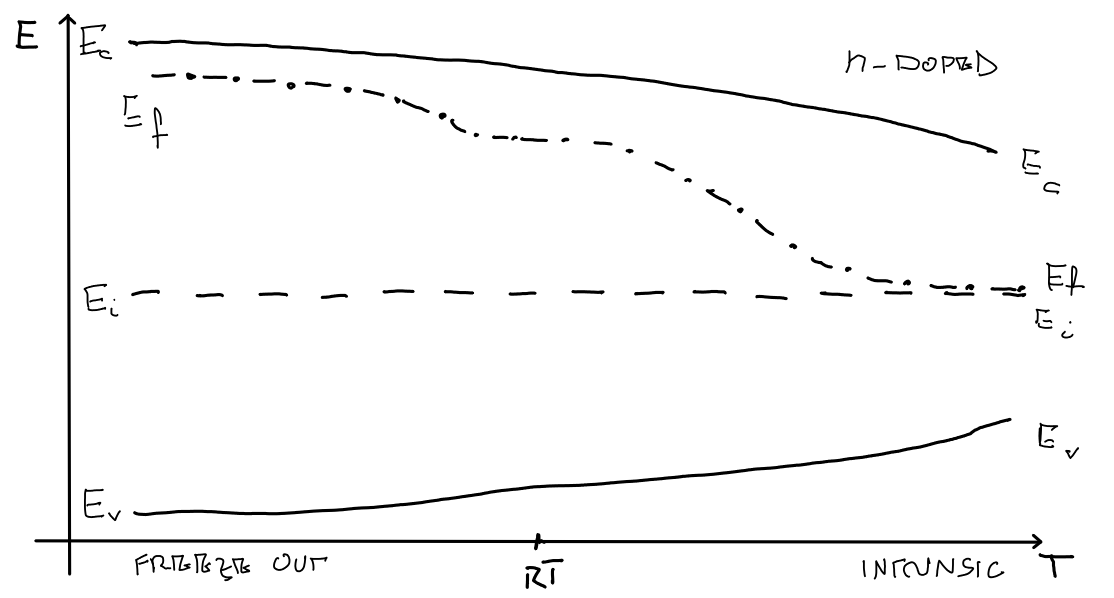
\includegraphics[width=0.5\textwidth]{E_f(T).png}
\end{wrapfigure}

With high T $E_g$ decreases and $E_f$ will move distant to $E_c$ following 1.23 until the hypothesis of negligible holes concentration decades and so at very high temperatures $E_f$ will tend asimptotically to $E_i$.\\
At very low temperature $E_f$ will increase until we reach the 0K where there is no conduction so $E_f$ has to stay a little bit higher than $E_d$.\\


%------------------------------------------------------------------------%
{\bf Low-temperature approssimation}\\

\begin{wrapfigure}{i}{0pt}
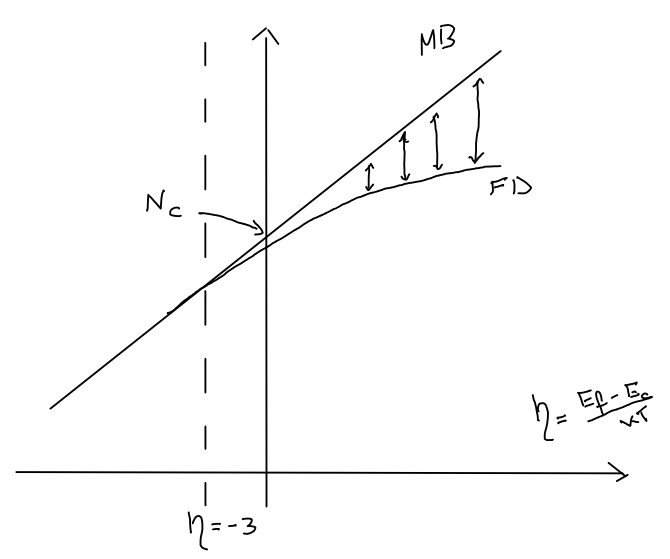
\includegraphics[width=0.35\textwidth]{mbfd.png}
\end{wrapfigure}

In the case of a material that has its Fermi level higher than the conduction band level we cannot use the M-B approximaton. The approximation we can do is a low-temperature one that trasforms the Fermi Dirac distribution into a step so
\begin{equation}
n=\int^{E_f}_{E_c}\frac{48\pi}{h^3}\sqrt{2m_t^2m_l}\sqrt{E-E_c}
\end{equation}
that multiplying and dividing the risult by $(kT)^{3/2}\sqrt{\pi}/2$ we obtain
\begin{equation}
n=N_c 2/3 \frac{2}{\sqrt{\pi}}\left(\frac{E_f-E_c}{kT}\right)^{3/2}=N_c 2/3 \frac{2}{\sqrt{\pi}}\eta^{3/2}
\end{equation}
In the graph above we can notice the difference between F-D and M-B distribution over $\eta$.\\
%------------------------------------------------------------------------%
\section{Current transport}
There are 2 most important mechanisms that generates current: drift and diffusion process.\\
Drift current is caused by the application of a electric field F; electrons are not only influenced by F but olso from scattering events so we can define a drift velocity (that is an average velocity) as 
\begin{equation}
v_d=\mu_n F
\end{equation}
So drift velocity is proportional to F with a constant $\mu_n$ called mobility that depends on doping concentration, temperature and dimensionality of the system taking in account all scattering events.It's important to note that in a bulk of doped Si if we are near the surface the mobility is much lower than the inside (dimensionality).\\
Mobility has a drop for Si around doping concentration of $\simeq 10^6 cm^{-3}$ beacuse at that level scattering with impurities becomes dominant in respect of thermal scattering.\\
Increasing too much F we arrive at the phenomena of velocity saturation ($\simeq 10^7 cm/s$) caused by scattering with high energetic optical phonons.\\
The density current caused by drift process is 
\begin{equation}
J=(qn\mu_n + qp\mu_p)F=\sigma F=F/\rho
\end{equation}
where $\sigma$ is the conductivity of the material and $\rho$ is the resistivity.\\

\begin{wrapfigure}{i}{0pt}
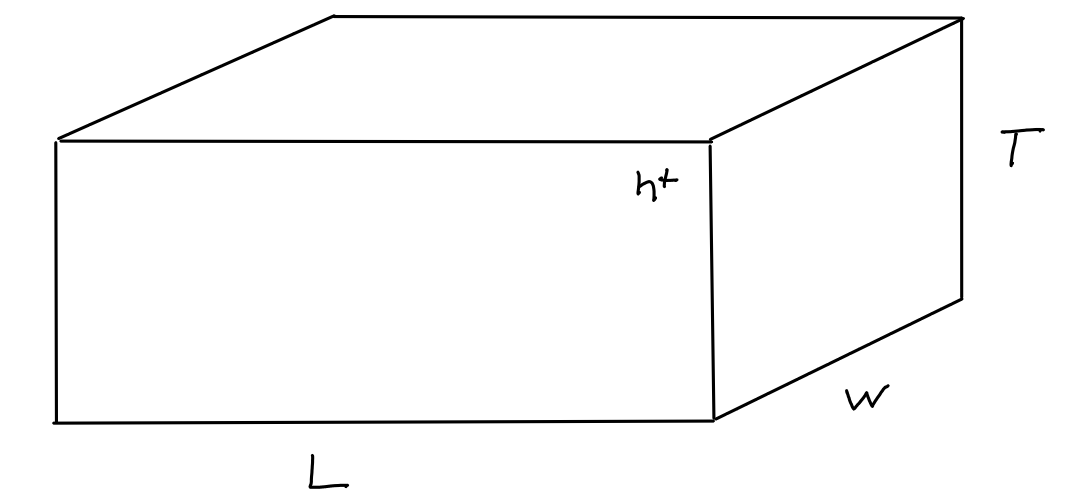
\includegraphics[width=0.4\textwidth]{shrho.png}
\end{wrapfigure}

When we calculate the resistivity of a block of doped silicon like in figure we define $\rho_{sh}=\rho/T$ as the sheet resistivity
\begin{equation}
R=\rho\frac{W}{LT}=\rho_{sh}\frac{W}{L} 
\end{equation}
Diffusion current is driven by a gradient of concentration so the density of current is 
\begin{equation}
J_n=qD_n\frac{dn}{dx} \ \ \ \ J_p=qD_p\frac{dp}{dx}
\end{equation}
where $D_n\ ,D_p$ are the diffusion coefficients defined by Einstein's relations as 
\begin{equation}
D_n=\mu_n\frac{kT}{q}\ \ \ D_p=\mu_p\frac{kT}{q}
\end{equation}
\newline
%------------------------------------------------------------------------%
\section{Bands "geography"}

\centering
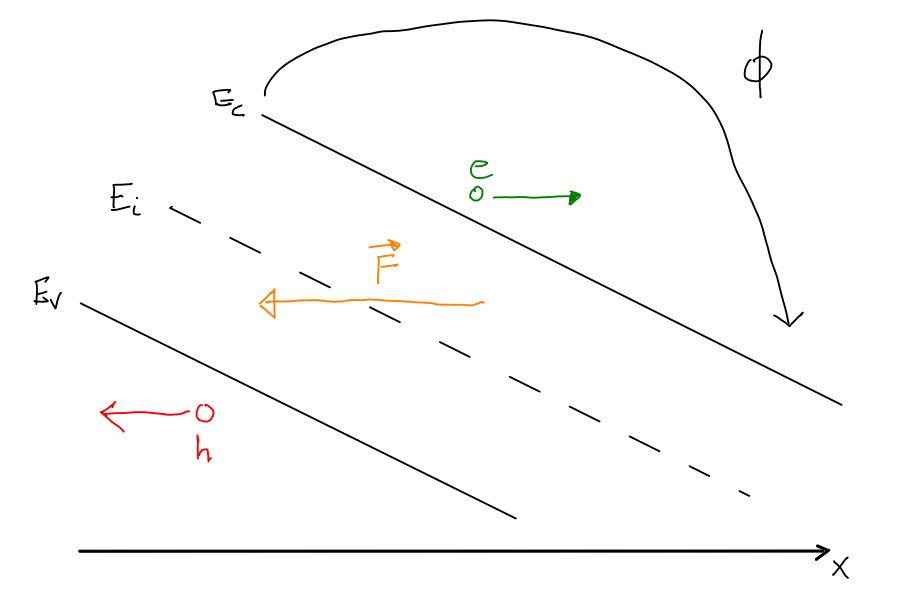
\includegraphics[width=0.5\textwidth]{bandsgeo.png}\\
\raggedright

We can obtain external potential $\phi$ as $\phi=\frac{-E_i(x)}{q}$.\\
The external potential increases in the direction the bands band downwards. The electric field is in the opposite direction of the growth of potential $\vec{F}=-\frac{d\phi}{dx}$.\\
Electrons move by drift in the opposite direction of F and holes in the same direction of F.\\

\centering
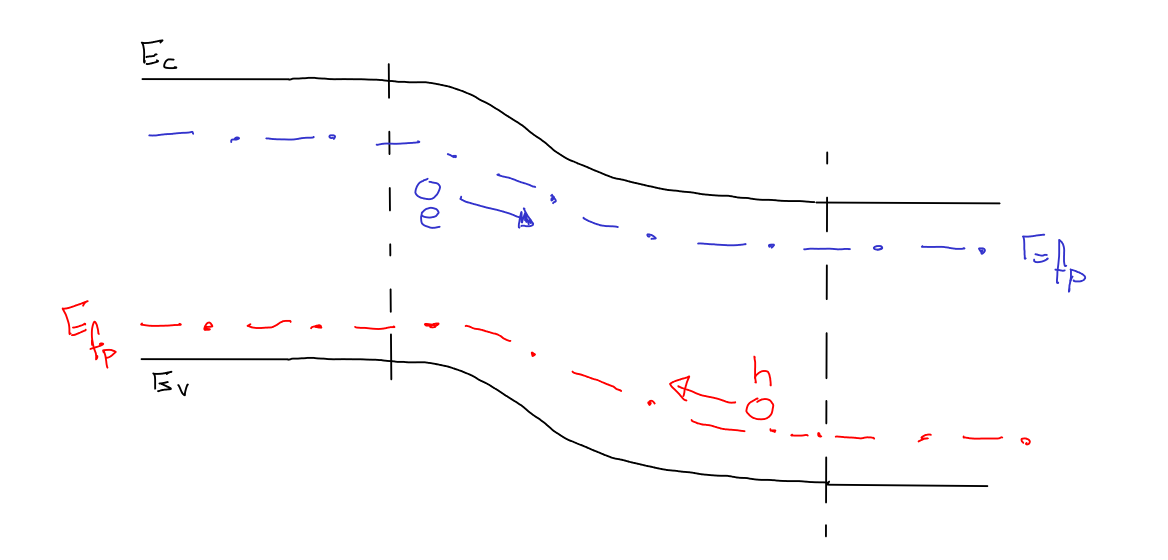
\includegraphics[width=0.5\textwidth]{bandsgeo2.png}\\
\raggedright

Without condition of thermal equilibrium electrons move from regions of high quasi fermi level to regions of low quasi fermi level and holes vice-versa.
%------------------------------------------------------------------------%
\section{Poisson equation}
Poisson equation is important to study the electrostatic of a system.\\
We can derive it from Maxwell's first law 
\begin{equation}
F=-\overrightarrow{\nabla}\phi\rightarrow F=-\frac{d\phi}{dx}
\end{equation}
and Gauss equation
\begin{equation}
\overrightarrow{\nabla}\overrightarrow{F}=\rho/\varepsilon_{Si}
\end{equation}
from witch we obtain considering that all charges we have in a semiconductor are holes, electrons and ionized donors 
\begin{equation}
\frac{d^2\phi}{dx^2}=-\rho/\varepsilon_{Si}=-\frac{q}{\varepsilon_{Si}}(p-n+N_d^+-N_a^-)
\end{equation}
In order to study the electrostatic of a system we have olso to know the coninutity equations of the electric field that are
\begin{equation}
F_{t1}=F_{t2} \Longleftrightarrow \epsilon_1F_{n1}-\epsilon_2F_{n2}=Q'_{int}
\end{equation}
\newline
%------------------------------------------------------------------------%
\section{Debye length}

Band banding is the phenomena caused by applying an electric field on a material at termodinamic equilibrium. This band banding causes different concentrations of e an h over the space so we can re-write the electron and holes concentrations taking in account the change of $\phi(x)$ over the space as
\begin{equation}
n=n_ie^{q\frac{\phi(x)-\phi_f}{kT}} \ \ \ p=n_ie^{q\frac{\phi_f-\phi(x)}{kT}}
\end{equation}
This band banding is tipically caused by the change of doping concentration over the space.With a smooth change of $N_d$ in a material we can assume that $n=N_d$.\\
Let's assume a step-like function in doping concentration in this case we cannot consider $n=N_d$ over the space beacuse this assumption will lead us to an infinite electric field.\\ 
Using Poisson equation and neglecting holes and ionized acceptors we can say that $N_d(x)=\hat{N_d}+\delta N_d(x)$ corrisponding to $\phi(x)=\hat{\phi}+\delta \phi(x)$ and assuming $\delta N_d<<N_d $ we can write
\begin{equation}
\frac{d^2\phi}{dx^2}=-\rho/\varepsilon_{Si}=-\frac{q}{\varepsilon_{Si}}(\hat{N_d}+\delta N_d(x)-n_ie^{q\frac{\hat{\phi}+\delta\phi(x)-\phi_f}{kT}})=-\frac{q}{\varepsilon_{Si}}(\hat{N_d}+\delta N_d(x)-\hat{N_d}e^{q\frac{\delta\phi(x)}{kT}})
\end{equation}  
we can write the first order expansion of the exponential term beacuse the exponent is small ($e^{q\frac{\delta\phi(x)}{kT}}\simeq 1+q\frac{\delta\phi(x)}{kT} $) obtaining the following differential equation
\begin{equation}
\frac{d^2\phi}{dx^2}=\frac{q^2\hat{N_d}}{\varepsilon_{Si}kT}\phi(x)-\frac{q}{\varepsilon_{Si}}\delta N_d(x)
\end{equation}
the solution of this equation give us an exponential decrease of the potential with a length called Debye length
\begin{equation}
L_D=\sqrt{\frac{\varepsilon_{Si}kT}{q^2N_d}}
\end{equation}
this will cause a net charge (both negative and positive near the discontinuity).\\

%------------------------------------------------------------------------%
\section{Quasi-Fermi levels}

\begin{wrapfigure}{i}{0pt}
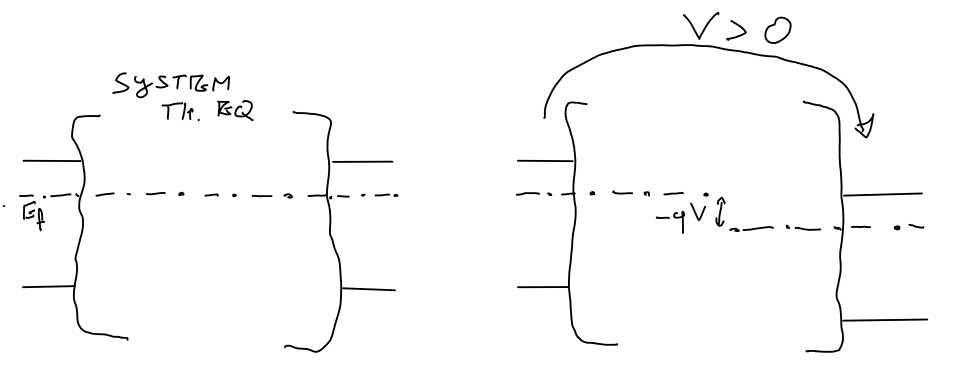
\includegraphics[width=0.4\textwidth]{perturbation.png}
\end{wrapfigure}

For having a net current transport (we're leaving the thermodinamic equilibrium hypotesis) we have to perturbe our system by for example applying at the contact \footnote{region of dispositive from witch we can externally apply a F, a good contact stays at th. eq.} a $V\neq 0$. 
As the figure shows  we can't introduce a $E_f$ level and so we cannot use the FD distribution. If the perturbation is weak we can recover all expressions of th.eq by introducing different Fermi levels both for e and h called quasi Fermi levels
\begin{equation}
n=n_ie^{\frac{E_{fn}-E_i}{kT}} \ \ \ \ \ \ p=n_ie^{\frac{E_i-E_{fp}}{kT}}
\end{equation}
so we can write the law of mass action generalized as 
\begin{equation}
pn=n_i^2e^{\frac{E_{fn}-E_{fp}}{kT}}
\end{equation}
Now let's try to analise the total current density of electrons. The formula has a strong dependance from the electrostatic potential (from F and n) so
\begin{equation}
J_n=-qn\mu_nF+qD_n\frac{dn}{dx}=-qn\mu_n\frac{d\phi}{dx}+qD_n\frac{d}{dx}\left(n_ie^{q\frac{\phi-\phi_f}{kT}}\right)=-qn\mu_n\frac{d\phi_f}{dx}
\end{equation} 
But since the Fermi potential is costant the result is 0 and it's obvius beacuse we assume th.eq. with formula (1.20).
If we substitute the (1.39) in n we obtain
\begin{equation}
J_n=-n\mu_n\frac{d\phi_{fn}}{dx}
\end{equation}
that isn't 0 beacuse $\phi_{fn}$ can change.\\
Electrons moves from the region of high quasi Fermi level to region of low quasi Fermi level, holes the opposite.
\newline
%------------------------------------------------------------------------%
\section{Equation of for e and h}

\centering
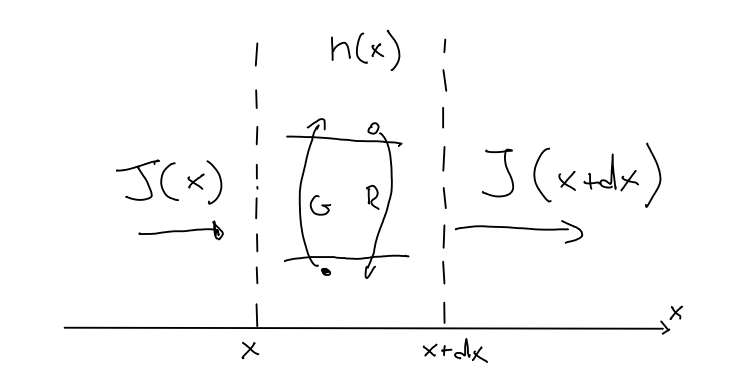
\includegraphics[width=0.4\textwidth]{continuityeq.png}\\
\raggedright

Let's consider the figure above if we make a ballace of charges between x and x+dx we have 
\begin{equation}
\frac{\partial n}{\partial t}dx=-J_n(x)/q+J_n(x+dx)/q+(G-R)dx
\end{equation}
where G and R are generation and ricombination processes per unit time per unit volume. If we expand at the first order $J(x+dx)\simeq J_n(x)+\frac{\partial J_n}{\partial x}dx $ and simplify the expression we have
\begin{equation}
\frac{\partial n}{\partial t}=\frac{1}{q}\frac{\partial J_n}{\partial x}+G-R \ \ \ \ \ \ \frac{\partial p}{\partial t}=-\frac{1}{q}\frac{\partial J_p}{\partial x}+G-R
\end{equation}
that are the continuity equation for electrons and hole current.\\
In a stationary system nothing change with time so subtractring the 2 equation we have 
\begin{equation}
\frac{1}{q}\frac{\partial(J_n+J_p)}{\partial x}=0
\end{equation}
so the sum of the 2 contributions of current from e and h stay costant. If we neglect G and R the 2 contrbutes are costant separatly.\\
G and R process restabilize equilibrium of a system if we perturb the minority carrier concentration. If we disturb majority carrier the system returns in equilibrium with a very short time costant.
Let's analyse the 2 case.\\ 

%------------------------------------------------------------------------%
\vspace{5mm}
{\bf Majority carrier perturbation}\\
Assume a n-doped material and let us add $\Delta n$ concentration of electrons. Using poisson equation we have
\begin{equation}
\frac{\partial \phi^2}{\partial x^2}=-\frac{q}{\varepsilon}\left(-n-\Delta n + N_d\right)=\frac{q\Delta n}{\varepsilon}=-\frac{dF}{dx} 
\end{equation}
from this result we obtain a field that has a linear dependence over the space that tends to move away the excess of charge with a drift current (no diffusion the concentration is costant) so using  1.44
\begin{equation}
\frac{\partial J_n}{\partial x}=qn\mu_n\frac{\partial F}{\partial x}
\end{equation}
\begin{equation}
\frac{\partial n}{\partial t}=\frac{1}{q}\frac{\partial J_n}{\partial x}=-\frac{1}{q}qn\mu_n\frac{q\Delta n}{\varepsilon}=-\frac{\Delta n}{\varepsilon \rho}
\end{equation}
solving this differential equation we have a solution that has an exponential dependence with $\varepsilon \rho$ that is called the dialectric relaxation time of the material; it's the time costant that the system use to return to its equilibrium ($\simeq ps$)\\

%------------------------------------------------------------------------%
\vspace{5mm}
{\bf Minority carrier perturbation}\\
The phenomena described for majority carrier concentration isn't valid for minority carrier. Considering a n-doped material like before the $\rho$ in equation 1.48 is very high (we are considering holes now) so the real result of the field is that attracts a concentration $\Delta n$ over $\Delta p$ creating a quasi-neutral region where G and R slowly decrease the 2 extra concentration.\\
In the processes of G and R in Si electrons cannot move thought the bandgap from CB to VB they need another particle to respect the conservation of momentum.\\

\begin{wrapfigure}{i}{0pt}
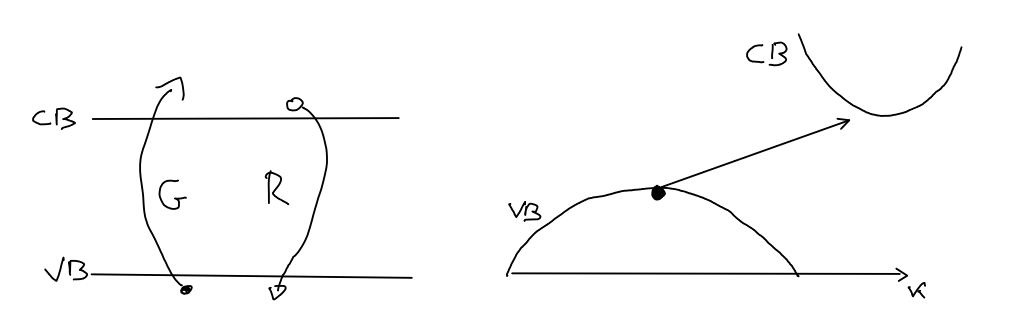
\includegraphics[width=0.4\textwidth]{srhp1.png}
\end{wrapfigure}

We need a difect of the cristal that creates another "band" in the bandgap this process called difect assisted and is described by Shockley-Reed-Hall theory.\\
The difect can only be empty or filled with one electron so there can be only 4 process: 1)Difect empty captures e from CB   2) Difect filled realeses an e to CB 3) Difect filled captures hole from VB 4) Difect empty realeses an hole from VB.

\begin{wrapfigure}{i}{0pt}
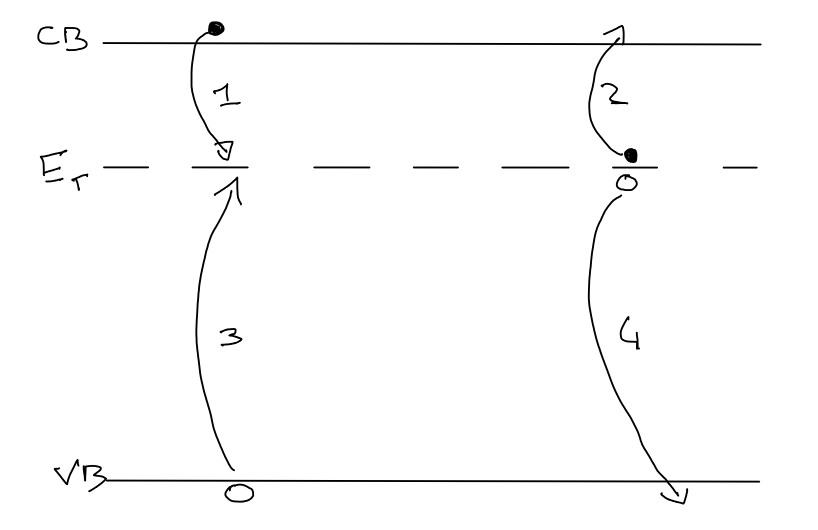
\includegraphics[width=0.4\textwidth]{srhp2.png}
\end{wrapfigure}

For R we need 1 and 3 for G 2 and 4.\\
The rate of 1 can be described as 
\begin{equation}
r_1=N_T(1-f(E_T))n(v_{th} \delta_n)
\end{equation}
where: $N_T$ is the total difect concentration ,f probability of the difect to be filled and the last term is a costant where $\delta_n$ is the capture crossection.\\
The rate of process 2 can be described as 
\begin{equation}
r_2=N_Tf(E_T)e_n
\end{equation}
where $e_n$ is a proportionality costant emission rate for e.
Under th.eq. $r_1=r_2$ and we can use the FD distribution for f. Under this condition we can calculate $e_n$ (and using the same consideration olso for process 3 and 4 and so obtaining $e_p$)
\begin{equation}
e_n=n_iv_{th}\delta_ne^{\frac{E_T-E_i}{kT}} \ \ \ \ \ \ e_p=n_iv_{th}\delta_pe^{\frac{E_i-E_T}{kT}}
\end{equation}
There is an exponential dependance if the difect is colser to the conduction band the process of release is higher; vice-versa the process of capture doesn't have this dependance beacuse the e has only to realese energy.\\
Under stationary condition $R=r_1-r_2=r_3-r_4$ from this we obtain $f(E_T)$ and we get the final result 
\begin{equation}
R=\frac{pn-n_i}{\tau_0\left[p+n+2n_iCosh(\frac{E_T-E_i}{kT})\right]}
\end{equation}
where $\tau_0=1/(v_{th}N_T\delta)$ and we've assumed $\delta_n=\delta_p=\delta$.\\

Re-writing the numerator using $n=n_ie^{(E_{fn}-E_i)/kT}$ $p=n_ie^{(E_{fp}-E_i)/kT}$ we can obtain that if $E_{fn}>E{fp}\rightarrow R>0$ and if $E_{fn}<E{fp}\rightarrow R<0$.\\
\vspace{5mm}
Looking at the graph of R in the 2 case major of less than zero we can make a few considerations

\centering
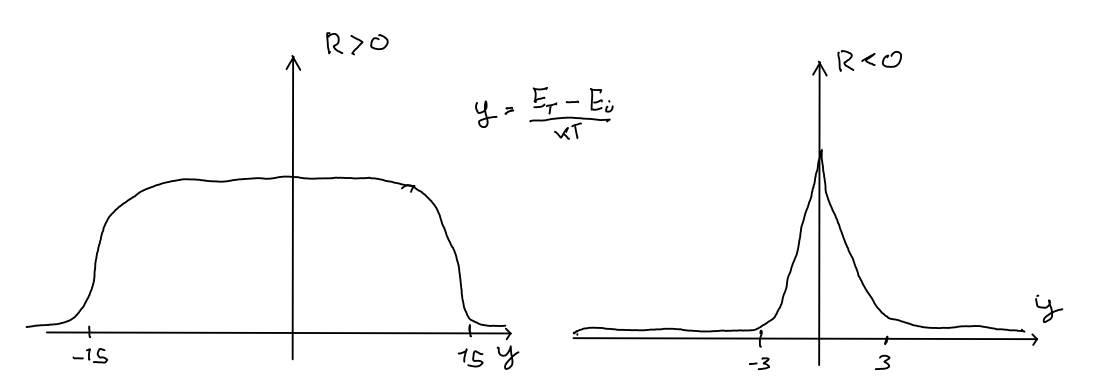
\includegraphics[width=0.4\textwidth]{RG.png}\\
\raggedright

\tab $R>0$ relevant part in the denominator is p+n but over 15 the Cosh becomes dominant so we get the drop.\\
\tab $R<0$ Cosh is always dominant so we have from the beginning a rapid drop beacuse p+n are few and the system is generating couples.\\
\vspace{5mm}
Phisical explanation can be given from a particular case.\\
We want to study only recombination so $R=\nu_1=\nu_3=(1-f(E_T))n=f(E_T)p$ so we can caluclate $f(E_T)=n/(n+p)$ and so $R=N_Tv_{th}\delta \frac{pn}{p+n}=\frac{pn}{\tau_0(n+p)}$ that is a semplification of the general formula we have a flat recombination rate beacuse 1,3 processes have only to loose energy the drop is caused by the growing relevance of 2 or 4 moving $E_T$ near to CB of VB.\\
The best position fot the difect is on the middle of the gap.\\
Maximum G is when p=n=0 so $G=-n_i/2\tau_0$.\\



%------------------------------------------------------------------------%
\section{Quasi-neutral condition}
%------------------------------------------------------------------------%

Under quasi-neutral condition $\Delta n +n_0=n$ and $\Delta p +p_0=p$ assuming low injection level ($\Delta n<<p_0+n_0$) we can neglect in the eq of R all the terms with "$\Delta$" so we obtain
\begin{equation}
R=\frac{\Delta n}{\tau_n}=\frac{(p_0+n_0)\Delta n}{\tau\left[p_0+n_0+2n_iCosh(\frac{E_T-E_i}{kT})\right]}=\frac{\Delta n}{\tau_n}
\end{equation}
if we suppose $E_T-E_i=0$ $\tau_n\simeq \tau_0=1/(N_Tv_{th}\delta)$\\
So the continuity equation for electrons becomes \footnote{Minus sign in the expression comes form G-R we are considering -R}
\begin{equation}
-\frac{d\Delta n}{dt}=R \rightarrow \Delta n \propto e^{-t/\tau_n}
\end{equation} 
where $\tau_n$ is dipendent on the quality of the material

        % Semiconductors basics
%------------------------------------------------------------------------%
%------------------------------------------------------------------------%
\chapter{Diodes}
%------------------------------------------------------------------------%
Diodes or pn junction are basically 2 zones of opposite doping polarity attached toghether.\\
To study pn junctions we have to make some simplyfing assumptions : we consider 1D materials with constant doping concentration and a step-like change of doping from p to n.\\
%------------------------------------------------------------------------%
\section{Built-in potential}
%------------------------------------------------------------------------%
\begin{wrapfigure}{i}{0pt}
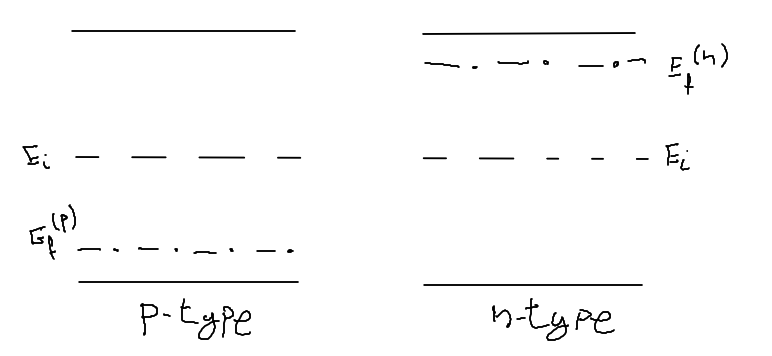
\includegraphics[width=0.4\textwidth]{pn1.png}
\end{wrapfigure}


Let's consider the 2 regions isolated from each other and under th.eq. We don't have a single Fermi level so depending on the zone we have 
\begin{equation}
E_i-E_f^{(p)}=kT\ln(\frac{N_a}{n_i}) \ \ \ \ \ \ \ E_f^{(n)}-E_i=kT\ln(\frac{N_d}{n_i})
\end{equation}
where $E_f^{(n/p)}$ is the Fermi level in that zone.\\

\begin{wrapfigure}{o}{0pt}
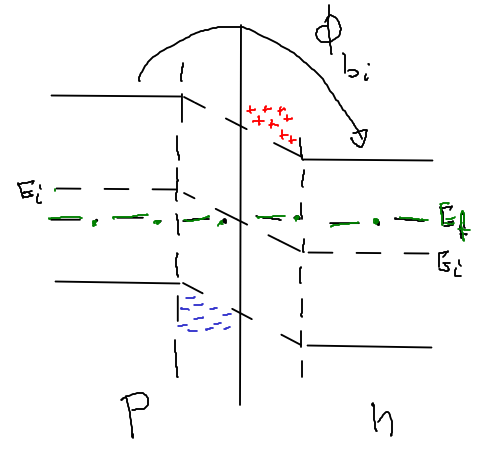
\includegraphics[width=0.25\textwidth]{pn2.png}
\end{wrapfigure}

When we put the 2 materials toghether there will be first a diffusion current and than also a drift current due to the band banding and the exposed charge; we will reach th.eq when the total current will be 0.\\Under th.eq we will have a costant Fermi level all over the space and a band banding at the interface. Far from the intarface we will reach zones where the bands are like the isolated case. The drop of electrostatic potential in the junction under th.eq is called built in potential or $\phi_{bi}$ and is 
\begin{equation}
q\phi_{bi}=(E_f^{(n)}-E_f^{(p)})|_{n.e}=kT\ln(\frac{N_aN_d}{n_i^2})
\end{equation} 
that is close to the $E_g$ of the material.\\
%------------------------------------------------------------------------%
\section{Depletion approximation}
%------------------------------------------------------------------------%
Beacuse the distance $E_f-E_c$ increase near the junction we have a exponential deacrease of n so in the transition region we can say that $n<<N_d$ and so $p<<N_a$.\\
From this we can say that the transition region is depleted of free carriers beacuse their concentration is negligible so this region is called depletion region.
%------------------------------------------------------------------------%
\section{Electrostatics of a pn junction}
%------------------------------------------------------------------------%

\begin{wrapfigure}{i}{0pt}
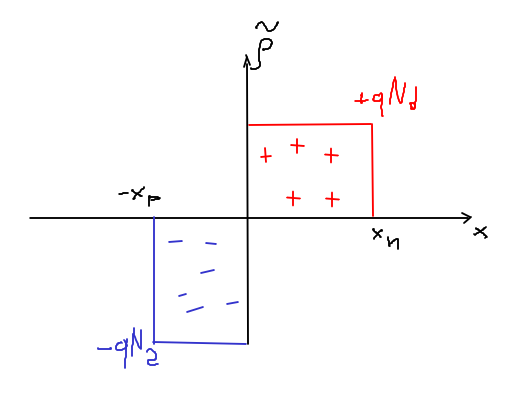
\includegraphics[width=0.35\textwidth]{pn3.png}
\end{wrapfigure}

We have to solve poisson equation in the depletion region so using depletion approximation and considering complete ionization
\begin{equation}
\frac{d\phi^2}{dx^2}=-\frac{q}{\varepsilon}(N_d-N_a)
\end{equation} 
and considering the concentration of fixed charges like the graph we can split the Poisson eq in 2 parts for $-x_p<x<0$ we have $\frac{d^2\phi}{dx^2}=\frac{q}{\varepsilon}N_a$ and for $0<x<x_n$ we have $\frac{d^2\phi}{dx^2}=-\frac{q}{\varepsilon}N_d$.\\
If we integrate both side of this equation and remembering that $F(x_n)=0$ we can deduce the electric field in the junction as 
\begin{equation}
\int^{x_n}_{x} d\frac{d\phi}{dx}=\int^{x_n}_{x}-\frac{q}{\varepsilon}N_d dx
\end{equation}

\centering
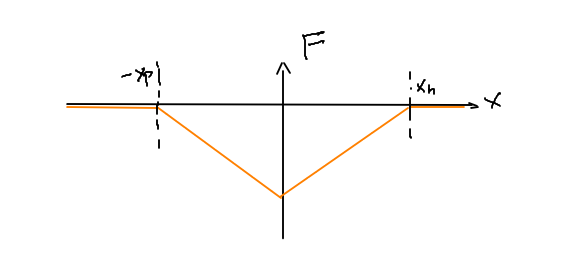
\includegraphics[width=0.35\textwidth]{pn4.png}\\
\raggedright

\begin{equation}
F(-x_p<x<0)=-\frac{qN_a}{\varepsilon}(x_p+x)\ \ \ \ \ \ \ \ F(0<x<x_n)=-\frac{qN_d}{\varepsilon}(x_n-x)
\end{equation}

\begin{wrapfigure}{i}{0pt}
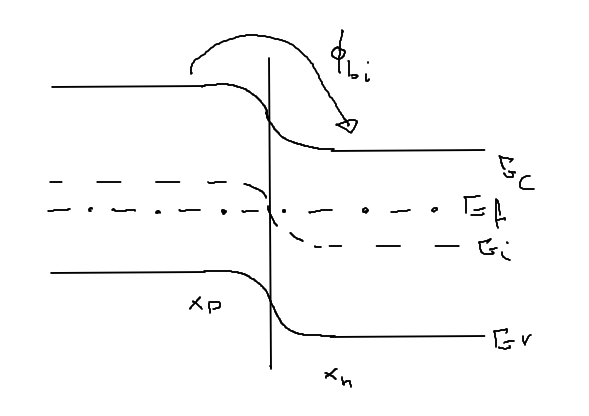
\includegraphics[width=0.3\textwidth]{pn5.png}
\end{wrapfigure}

for continuity equations of the electric field the F must be continuos in 0 so from this condition we get that $N_ax_p=N_dx_n$ that means that the total charge in the depletion area is 0 (from Gauss law also).\\
Integrating again both parts of the equation of the field we finally obtain the potential over the space that has a parabolic dependance
\begin{equation}
\phi(-x_p<x<0)=\phi(-x_p)+\frac{qN_a}{2\varepsilon}(x+x_p)^2 \ \ \ \ \ \ \ \ \phi(0<x<x_n)=\phi(x_n)-\frac{qN_d}{2\varepsilon}(x_n-x)^2
\end{equation}


To know $x_n$ and $x_p$ we have to set some boundary condition: $\phi$ must be continuos in 0, and $N_ax_p=N_dx_n$ from this 2 condition we get 
\begin{equation}
x_n=\sqrt{\frac{2\varepsilon}{q}\phi_{bi}(\frac{1}{N_a}+\frac{1}{N_d})}\times \frac{N_a}{N_a+N_d}\ \ \ \ \ \ \ 
x_p=\sqrt{\frac{2\varepsilon}{q}\phi_{bi}(\frac{1}{N_a}+\frac{1}{N_d})}\times \frac{N_d}{N_a+N_d}\ \ \ \ \ \ \ 
W=\sqrt{\frac{2\varepsilon}{q}\phi_{bi}(\frac{1}{N_a}+\frac{1}{N_d})}
\end{equation}
\vspace{5mm}
Order of magnitude for the depletion layer given N the doping concentration of the less doped zone:

\begin{table}[]
\centering
\begin{tabular}{|l|l|}
\hline
$N_{d/a}$ & $W_d$ \\ \hline
$10^{16}$ & 300nm \\ \hline
$10^{17}$ & 100nm \\ \hline
$10^{18}$ & 10nm \\ \hline
\end{tabular}
\end{table}

\vspace{15mm}

%------------------------------------------------------------------------%
\section{Unilateral Junction}
%------------------------------------------------------------------------%

\begin{wrapfigure}{i}{0pt}
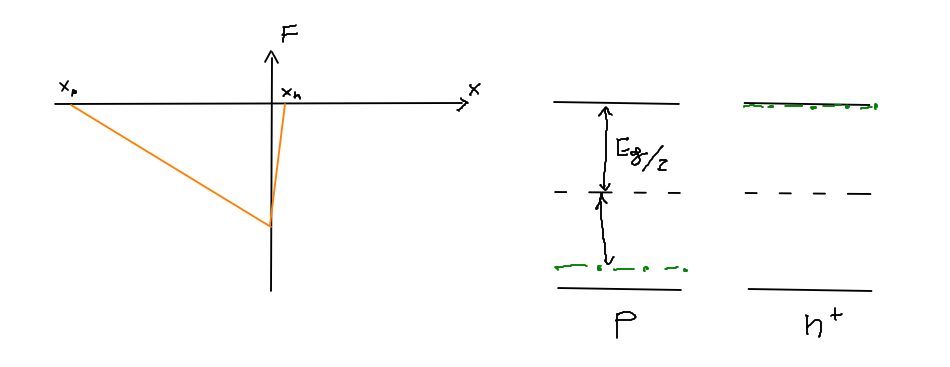
\includegraphics[width=0.6\textwidth]{pn6.png}
\end{wrapfigure}

Let's consider a junction $n^+p$ so the depletion area is almost all in the less doped material and so the electric field. We can make some approximation that the depletion area is almost in the p zone and that the Fermi level of the $n^+$ zone is almost at $E_c$ so this lead us to 
\begin{equation}
W\simeq x_p \ \ \ \ \ q\phi_{bi}\simeq E_g/2 + kT\ln(\frac{N_a}{n_i})
\end{equation}

%------------------------------------------------------------------------%
\section{Bias}
%------------------------------------------------------------------------%


\centering
\fbox{\begin{minipage}{40em}
To better uderstand this paragraph draw the below graphs with also the electric field due to the external applied voltage.
\end{minipage}}
\raggedright


\vspace{3mm}
{\bf Forward Bias}\\

\centering
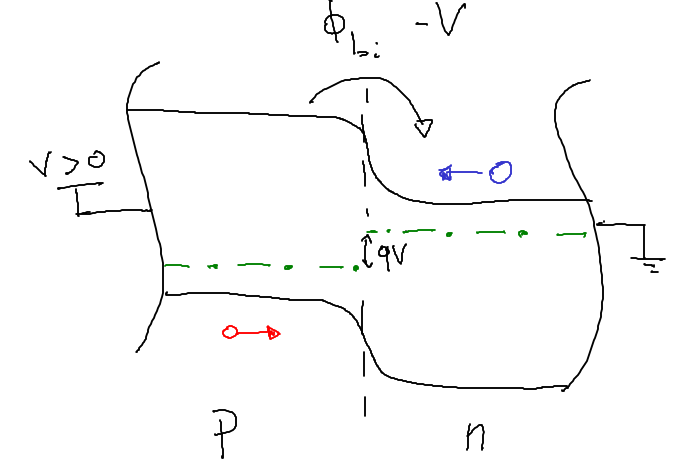
\includegraphics[width=0.35\textwidth]{pn7.png}\\
\raggedright

Applying a external voltage like in figure we are reducing the total voltage drop over the junction. There will be a net flow of electrons from left to right that is a current by diffusion that will be large since the flow of current is due to majority carriers.\\
{\bf Revers Bias}\\

\centering
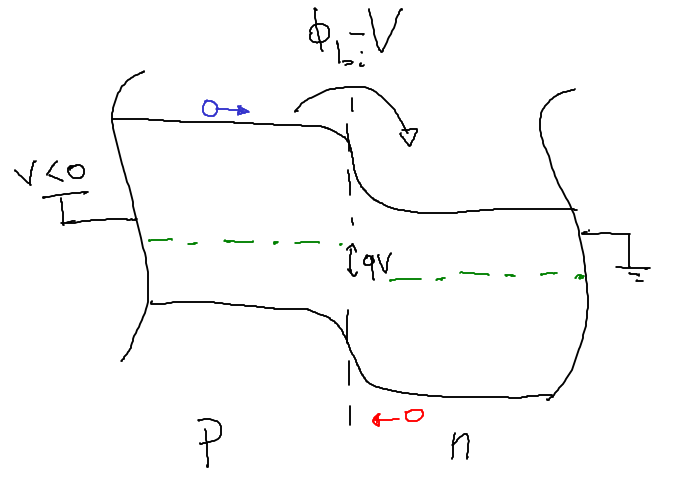
\includegraphics[width=0.35\textwidth]{pn8.png}\\
\raggedright

In this case $V<0$ electrons and holes move for drift the total voltage drop will be greater than the built in. The flow of current is given by minority carrier so small I.\\

%------------------------------------------------------------------------%
\section{The V-I characteristic of pn }
%------------------------------------------------------------------------%
We want to investigate on foward bias electrostatic but we have to make some other simplyfing assumption: the contacts of our junction are at th.eq. and looking to the n region moving closer to the contact (from the interface) we will enter in a region where electrons are majority carrier. Beacuse we are injecting holes in that region we will have $p=p_{n0}+\Delta p$ so a region of quasi-equilibrium.\\
If we assume stationarity and that G and R process are negligible and so the $J_n=n\mu_n \frac{dE_{fn}}{dx}=cost$. \\
Beacuse n isn't costant all over the space (space of all the diod first n minority than majority) $\frac{dE_{fn}}{dx}$ will change over the space.\\
Being the grandient of n very small near the contacts $E_{fn}$ will be almost flat as conduction and valence bands in that region.
The final graph is this 

\centering
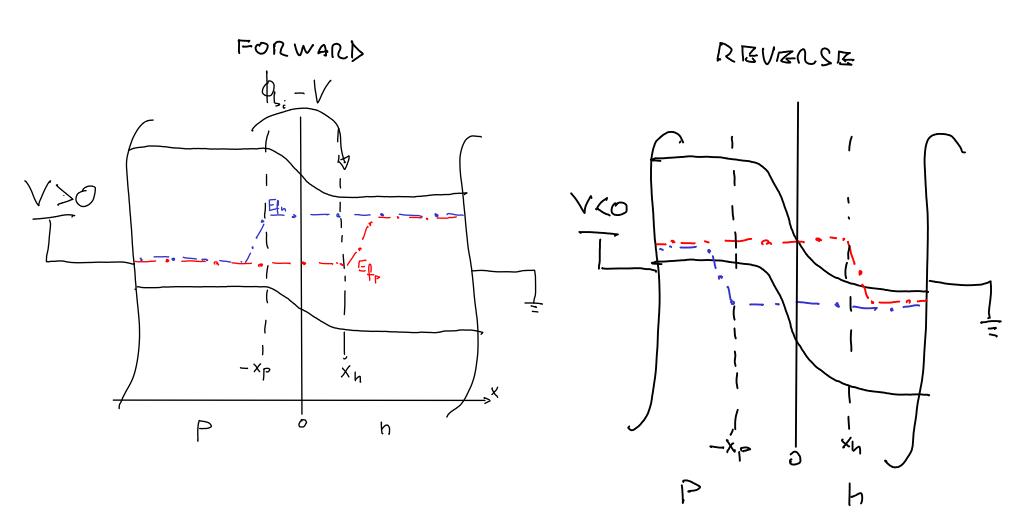
\includegraphics[width=0.6\textwidth]{pn9.png}\\
\raggedright

we have 2 region of quasi-equilibrium and a transition region that is depleted from free charges.\\
\vspace{3mm}
We can divide the a zone in 3 regions and analyse the the two factors n and $\frac{dE_{fn}}{dx}$:\\ 
\tab {Near the contact: small gradient of n so also small change of $\frac{dE_{fn}}{dx}$ that we can assume quasi-constant.\\}
\tab Depleted region: free carriers are negligible and so "constant" all over that zone so also here quasi-constant $\frac{dE_{fn}}{dx}$.\\
\tab Opposite transition region: here the values of n rapidally drops until it reachs the equilibrum value so there will be a noticeble $\frac{dE_{fn}}{dx}$.\\
\vspace{3mm}  
This is the same result of electrostatic without bias so the depletion region will be
\begin{equation}
W=\sqrt{\frac{2\varepsilon}{q}(\phi_{bi}-V)(\frac{1}{N_a}+\frac{1}{N_d})}
\end{equation}
$E_{fn}$ remains almost\footnote{if $E_{fn}$ is constant its gradient is zero and there is no current flowing according to previous expressions} costant until $-x_p$ but n changes beacuse $E_c$ moves upwards.\\
For reverse bias we have to follow the same path of forward bias arriving at the graph above.\\
Bands are flat near the contact beacuse we suppose (1) quasi-neutral region under (2) low level of injection with (3) costant doping and (4) negligible gradient of quasi-Fermi levels; if one of this supposition falls the bands will no more be flat.\\
\vspace{5mm}
\label{cont.eq}
Now we want to know the quasi-Fermi level in the minority region.
We know that at $x=x_n$ $n\simeq N_d$ and for the law of mass action generalized $p=\frac{n_i^2}{N_d}e^{\frac{E_{fn}-E_{fp}}{kT}}\simeq p_{n0}e^{\frac{qV}{kT}}$ and at $x=-x_p$ with the same passages we obtain $n\simeq n_{p0}e^{\frac{qV}{kT}}$. Now we can solve the continuity equation only in the quasi-neutral region. \\
Beacuse the bands are flat we have only diffusion so $J_n=qD_n \frac{dn}{dx}$ and $G-R=\frac{-\Delta n}{\tau_n}$ from this two in the coninuity equations under stationary conditions ($0=\frac{1}{q}\frac{\partial J_n}{\partial x}+G-R$) we get
\begin{equation}
\frac{d^2\Delta n}{dx^2}-\frac{\Delta n}{L_n^2}=0
\end{equation} 
where $L_n=\sqrt{D_n\tau_n}$ is the diffusion length of electrons in the quasi neutral p-region. Introducing the system of coordinate like in figure (where $W_p$ is the end of the quasi-neutral p region and so of the device) we can solve this differential equation.

\begin{wrapfigure}{i}{0pt}
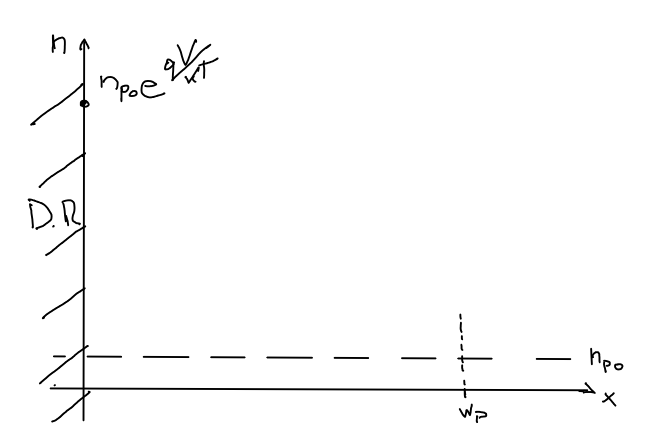
\includegraphics[width=0.45\textwidth]{pn10.png}
\end{wrapfigure}

Solving that as a polynomial we get $\lambda^2-\frac{1}{L_n^2}=0\leftarrow \lambda=\pm\frac{1}{L_n}$ so we get two exponential terms that are $\Delta n(x)=Ae^{\frac{x}{L_n}}+Be^{-\frac{x}{L_n}}$ using the boundary condition $\Delta n(0)=n_{p0}(e^{\frac{qV}{kT}}-1)$ and $\Delta n(W_p)=0$ we arrive at
\begin{equation}
\Delta n(x)=n_{p0}(e^{\frac{qV}{kT}}-1)\frac{\sinh(\frac{W_p-x}{L_n})}{\sinh(\frac{W_p}{L_n})}
\end{equation}
Having only diffusion processes we can know the current but we are intrested only\footnote{ The sum of electron and holes current will be constant since we are in a stationary condition so we keep interest only in one section of the device. We don't want to know the currents graphs in function of space in a rigorous way} in $J_n(0)$ at the edge of the quasi-neutral region so 
\begin{equation}
J_n(0)=(qD_n \frac{d\Delta n}{dx})|_{x=0}=-\frac{qD_nn_{p0}}{L_n\tanh(W_p/L_n)}(e^{\frac{qV}{kT}}-1)
\end{equation}
so in general the total current in the pn junction is 
\begin{equation}
J=[\frac{qD_nn_{p0}}{L_n\tanh(W_p/L_n)}+\frac{qD_pp_{n0}}{L_p\tanh(W_n/L_p)}](e^{\frac{qV}{kT}}-1)=J_0(e^{\frac{qV}{kT}}-1)
\end{equation}

\begin{wrapfigure}{i}{0pt}
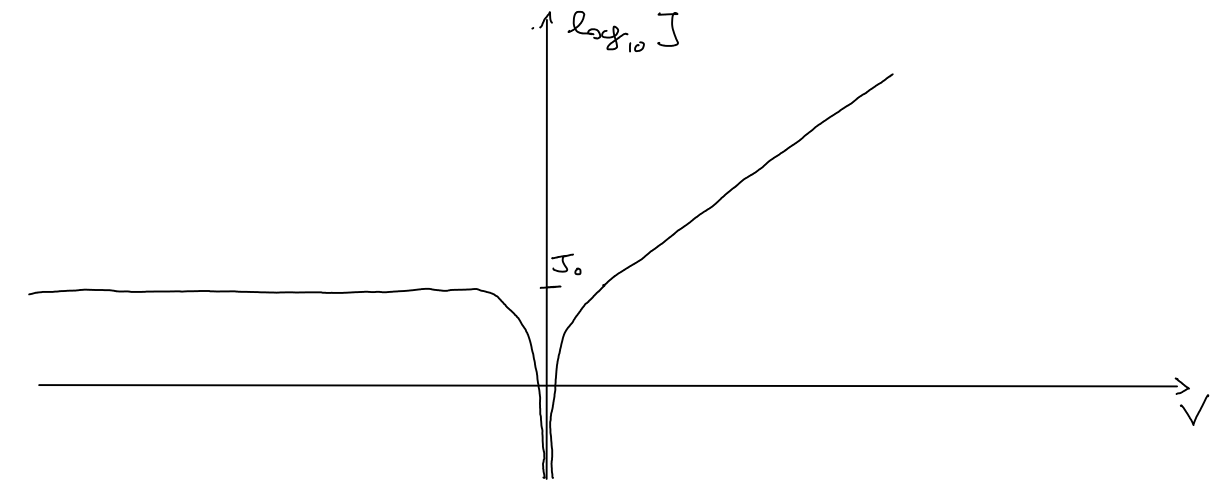
\includegraphics[width=0.35\textwidth]{pn11.png}
\end{wrapfigure}


If $V>>kT/q$ we can neglect 1 and plot a log-log scale of this characteristic that is 
\begin{equation}
\log(J)=log(J_0)+\frac{qV}{kT\ln(10)}
\end{equation}
One important parameter of the characteristic is the slope in foward bias that is $kT/q \ln(10)=60mV/dec \ @RT$.\\
\vspace{5mm}
The dominant contribute to the current is from the zone less doped like in the electrostatic.\\
If we have a $n^+-p$ junction the dominant flow is $J_n$; electron flowing through the p-region injected to n-region. Current density dominated by the less doped zone minority carriers.

%------------------------------------------------------------------------%
\section{Wide and narrow base diode}
%------------------------------------------------------------------------%

\centering
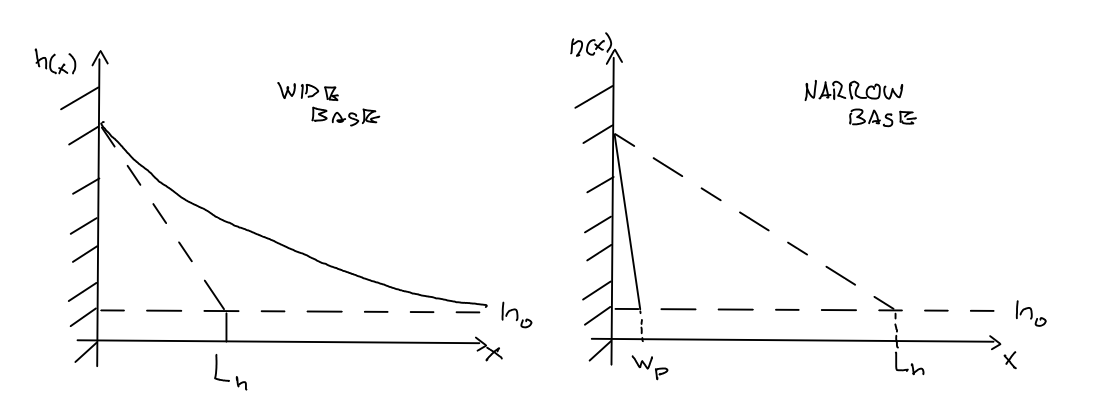
\includegraphics[width=0.65\textwidth]{pn12.png}\\
\raggedright

If we have a wide-base diode if $W_p>>L_n$ so we can approximate as follow the expression of charge and of current density 
\begin{equation}
\Delta n(x)=n_{p0}(e^{\frac{qV}{kT}}-1)e^{\frac{-x}{L_n}} \ \ \ \ \ \ \ J_n=\frac{qD_nn_{p0}(e^{\frac{qV}{kT}}-1)}{L_n}
\end{equation}


If we have a narrow-base diode if $W_p<<L_n$ so we can approximate as follow the expression of charge and of current density
\begin{equation}
\Delta n(x)=n_{p0}(e^{\frac{qV}{kT}}-1)\frac{W_p-x}{W_p}\ \ \ \ \ \ \ \ \ J_n=\frac{qD_nn_{p0}(e^{\frac{qV}{kT}}-1)}{W_p}
\end{equation}


\begin{wrapfigure}{i}{0pt}
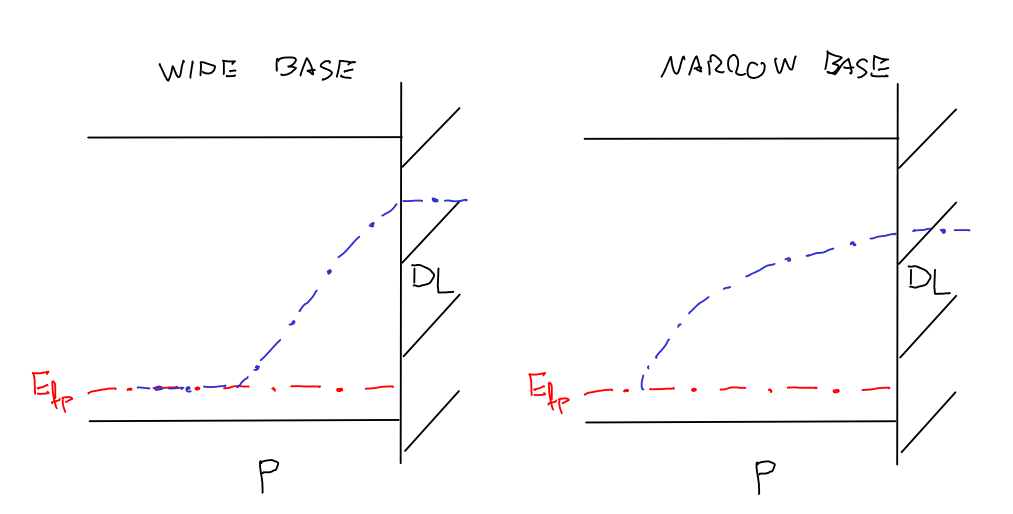
\includegraphics[width=0.35\textwidth]{wbnb.png}
\end{wrapfigure}

In a wide base diode n(x) decrease exponentially in the p region therefore $E_{fn}$ will decrease linearly with a slope of $kT/L_n$ and after the intersection with $E_{fn}$ it will be costant .\\
For a narrow base the decrease of $E_{fn}$ will be logaritmic beacuse n(x) decreases linearly.\\
In the quasi neutral p (n) region we have less electrons (holes) than in all other zone so the highest resistivity. The limit for conduction is given by the quasi-neutral region where we have less concentration of minority carriers; this is why the pn junction is called a minority carriers device , the limit for current transport is given by minority carriers.\\
\vspace{5mm}

\raggedright
\fbox{\begin{minipage}{40em}
Consider a narrow base diod in reverse bias. 
Increasing the negative voltage applied we increase the depletion layer reducing the width of the quasi neutral region. The reverse current will increase due to the increase of the slope of carriers.
\end{minipage}}
\raggedright

\raggedleft
\fbox{\begin{minipage}{40em}
Looking at the two expressions of the current in wide and narrow base case we can notice that the $J_0$ stays constant changing the length of the device if we consider a wide base diode but if we consider a narrow base one $J_0$ will increase hyperbolically (as 1/x) reducing W.\\
This is due to the fact that the current is purely diffusive and reducing the length means to increase the gradient of carriers and so the current. 
\end{minipage}}
\raggedright


\subsection{Current profile}
%------------------------------------------------------------------------%
{\bf Wide base forward bias}\\
The exponential behaviour of the minority will be followed by a consequent increase of majority charges in order to mantain the region quasi-neutral. In the depletion layer a connection between the 2 region. Minority carriers moves for diffusion but majority carrier moves for drift beacuse there is a small gradient of $E_{fn}$ that let electrons move from right to left.

\centering
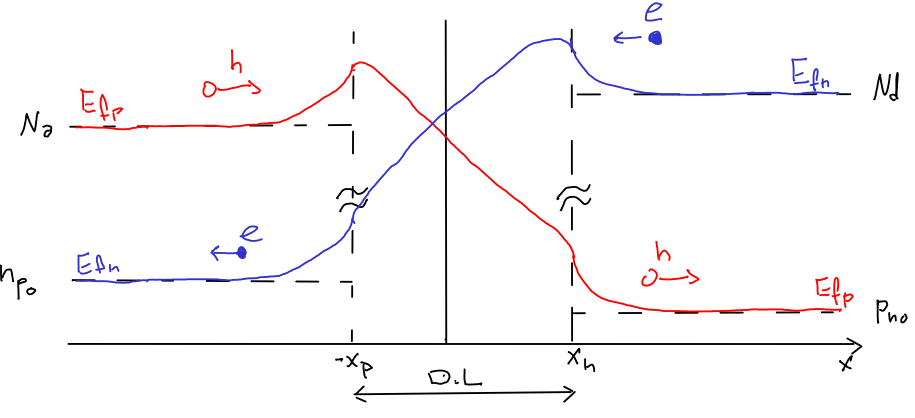
\includegraphics[width=0.5\textwidth]{nxfvb.png}\\
\raggedright

To know $J_n$ in n region we have to remember that under stationary condition (so in quasi neutral region) $J_n+J_p=const$. Also we remember that under stationary conditions and neglecting G-R both current contributions are constant. From this considerations we can draw the graph of $J_n,J_p$ over the space.\\

\centering
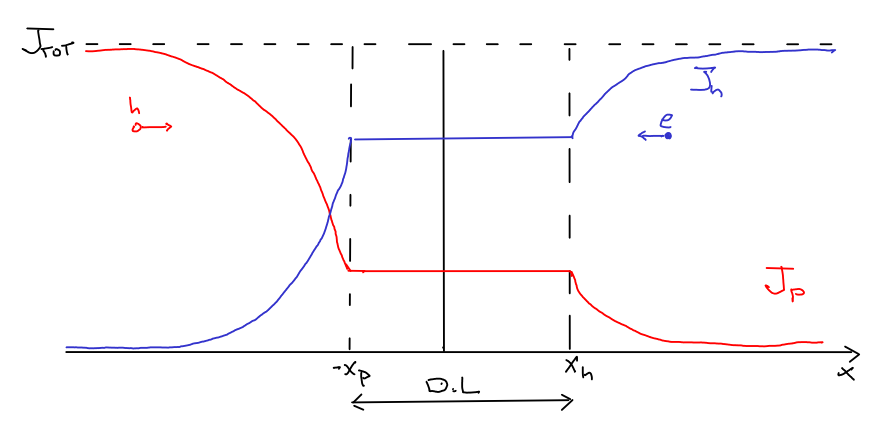
\includegraphics[width=0.5\textwidth]{wbfbJ.png}\\
\raggedright

{\bf Wide base reverse bias}\\
Same path of before : minority carrier in quasi neutral regions decrease before the depletion layer so this phenomena will be copied by the majority carrier in order to mantain quasi-neutrality.

\centering
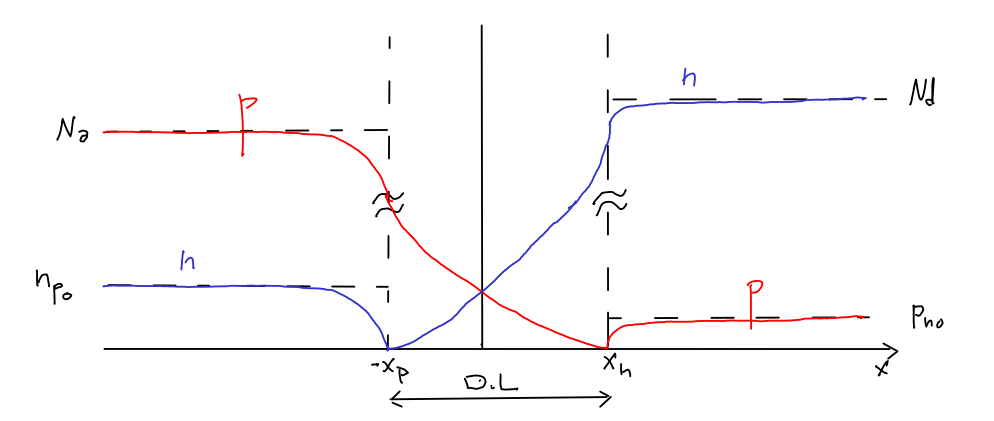
\includegraphics[width=0.5\textwidth]{rbwb.png}\\
\raggedright

Knowing $J_n+J_p=const$ in stationary conditions and that if we neglect also G-R process we have both currents constat we obtain the following graph.

\centering
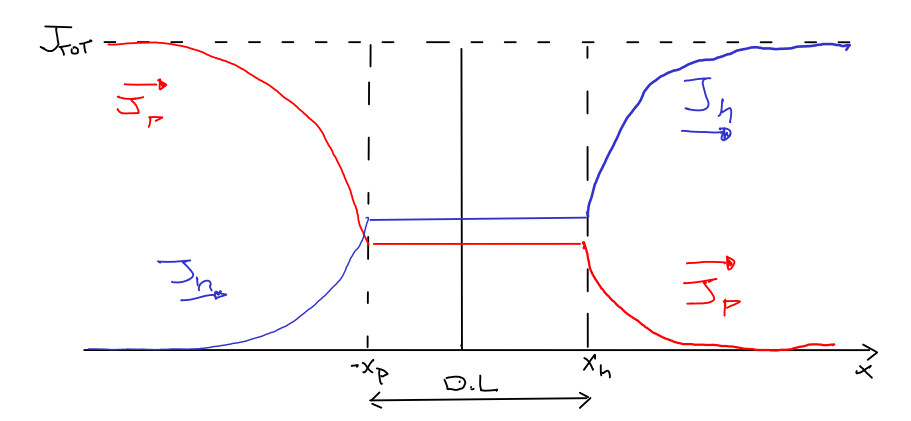
\includegraphics[width=0.5\textwidth]{wbrb.png}\\
\raggedright

The flow of holes becomes zero at n contact but than in grows for generation processes.\\
We have the same behaviour of the current both in reverse and in forward bias but $J_{tot}$ changes of orders of magnitude. As before minority carriers move by diffusion, majority by drift and in the depletion layer we have movement by drift.\\
\vspace{5mm}


{\bf Narrow base forward bias}\\
Linear increase of minority carriers so also majority in order to mantain the region quasi-neutral.\\

\centering
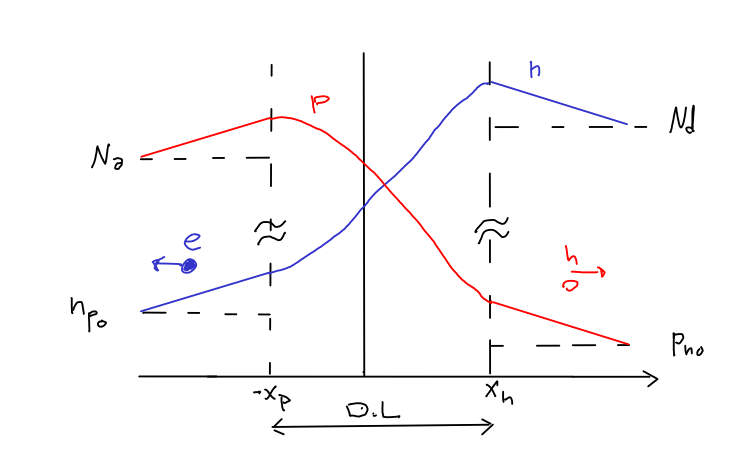
\includegraphics[width=0.5\textwidth]{nbfb.png}\\
\raggedright

The derivate of a linear dependence is constat so $J_n$ and $J_p$ remain constat. There is no space to G-R process beacuse the device is much shorter than $L_n$ so all generation and ricombination process are at the contacts.\\


\centering
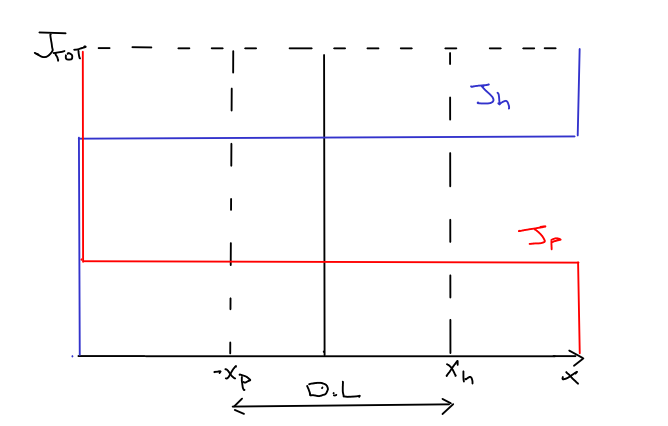
\includegraphics[width=0.4\textwidth]{nbJf.png}\\
\raggedright

{\bf Narrow base reverse bias}\\
With the same path of before we arrive at

\centering
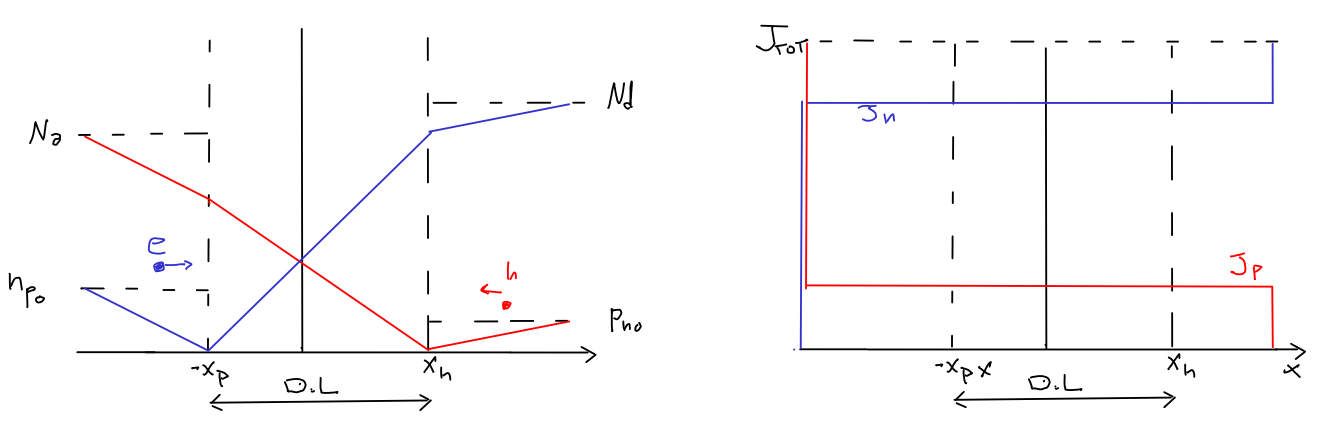
\includegraphics[width=0.85\textwidth]{nwall.png}\\
\raggedright

\centering
\fbox{\begin{minipage}{40em}
If we take into account a pn-j with dopings $N_a=10^{16}$, $N_d=10^{17}$ we get a diffusion lenght $L_n\simeq 310\mu m$, $L_p\simeq 110\mu m$ so it's unlikely to have a wide base diode in our integrated circuits.\\
G-R effects in modern integrated devices are secondary effects that takes place only at low current.
\end{minipage}}
\raggedright

\centering
\fbox{\begin{minipage}{40em}
Orders of magnitude for $J_0$ with $W=1\mu m$ in case of a wide base diod is $1 \ pA/cm^2$ ,for narrow base $1 \ nA/cm^2$
\end{minipage}}
\raggedright

\centering
\fbox{\begin{minipage}{40em}
All graphs are refered to a $p-n^+$ junction we can say that based on the concentration of carriers and also from the currents densities since the dominant contribution is always the one coming from electrons that are the minority carriers of the less doped zone.
\end{minipage}}
\raggedright

%------------------------------------------------------------------------%
\section{T change}
%------------------------------------------------------------------------%
Let's consider a pn junction in foward bias $J=J_0(e^{\frac{qV}{kT}}-1)\simeq J_0e^{\frac{qV}{kT}}$. If we increase the T the slope of the straight part will increase for the exponential term (be careful to units in the graph the line becomes flatter) but also $J_0=\frac{qD_nn_i^2}{N_aL_n}$ will increase for his strong dependance with temperature caused by $n_i^2\propto T^3e^{-\alpha/T}$.

\begin{wrapfigure}{i}{0pt}
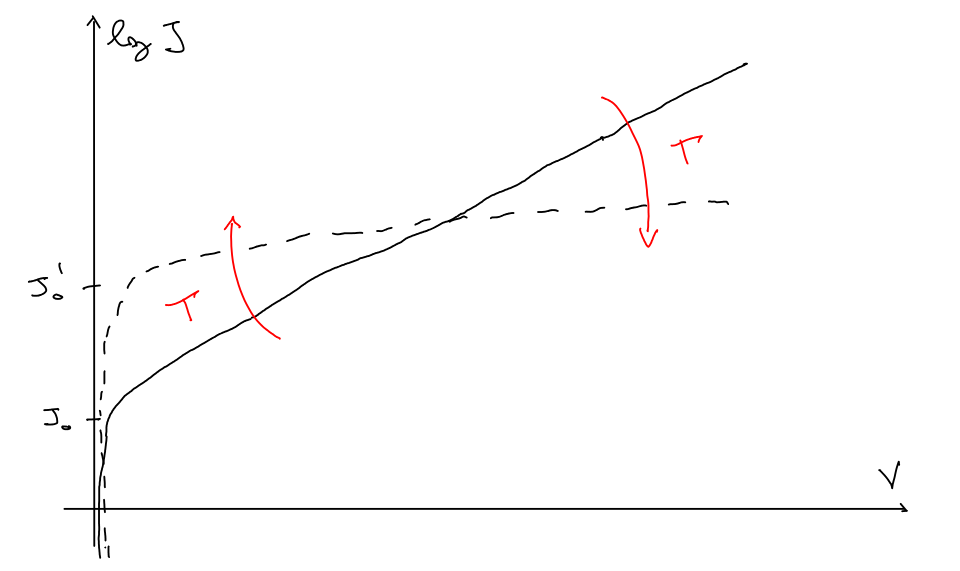
\includegraphics[width=0.5\textwidth]{JwithT.png}
\end{wrapfigure}

So with the increase of T we can have both an increase or a decrease of voltage corrisponding a fixed J. We have to find the typical regime of our device so from $J=J_0e^{\frac{qV}{kT}}$ we extract the voltage as $V=\frac{kT}{q}\ln(J/J_0)$ with J a fixed current. Now we cand derivate obtaining

\begin{equation}
\frac{dV}{dT}= \frac{k}{q}\ln(J/J_0)+\frac{kT}{q}J_0/J \frac{-J \frac{dJ_0}{dT}}{J_0^2}=V/T-\frac{kT}{q}\frac{dJ_0}{dT}\frac{1}{J_0}
\end{equation}

for semplicity we can hilight $J_0$ dependences on temperature writing $J_0=aT^\gamma e^{-E_g/2kT}$ so we obtain that $\frac{dJ_0}{dT}=J_0\gamma/T+J_0[-\frac{dE_g}{dT}\frac{1}{kT}] + J_0 \frac{E_g}{kT^2}$ so coming back at voltage we obtain

\begin{equation}
\frac{dV}{dT}=(V-\frac{E_g}{q})\frac{1}{T}-\frac{k\gamma}{q} + \frac{1}{q}\frac{dE_g}{dT}
\end{equation}

Since our typical $V\simeq0.6/0.7$ there are all negative terms so we are in the firs zone where we find a decrease of voltage w.r.t an increase of the temperature ( at RT $dV/dT\simeq -1.9mV/K$)

%------------------------------------------------------------------------%
\section{Second order effects on current}
%------------------------------------------------------------------------%
There are some phenomena that we have to consider in order to make more realistic the J-V graph of a pn junction.
%------------------------------------------------------------------------%
\subsection{Low current regime}

\begin{wrapfigure}{i}{0pt}
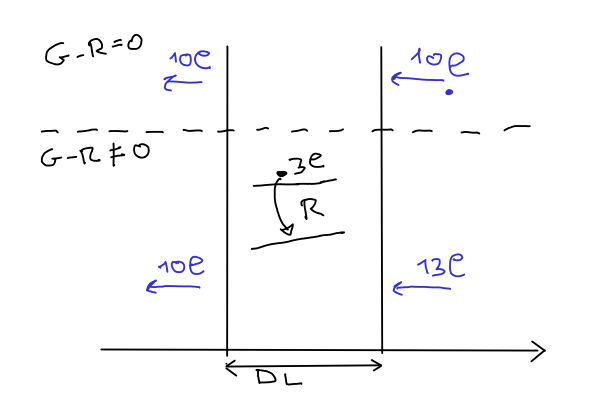
\includegraphics[width=0.35\textwidth]{Rdl.png}
\end{wrapfigure}

We have always neglected the G-R in the depletion layer but now we have to make some considerations.\\
Under reverse bias $E_{fn}<E_{fp}$ so there will be some generation processes, knowing the quasi-Fermi level and using the law of mass action generalized we can write the SRH R coefficient as
\begin{equation}
R=\frac{n_i^2(e^{qV/kT}-1)}{\tau_0(p+n+2n_i Ch((E_t-E_i)/(kT))}
\end{equation} 
so the sign of the voltage applied V change the sign of R.\\
Refering to forward bias the impact of R is that from majority region there will be more electron moving to the depletion region beacuse of minority constrain of the pn junction. 
So we aspect a larger current under foward bias where $R\simeq \frac{n_i^2(e^{\frac{qV}{kT}}-1)}{\tau_0[p+n]}$ to get the worst case we take p=n so R will be maximum and we get $R= \frac{n_i(e^{\frac{qV}{2kT}})}{2\tau_0}$.\\
Under forward bias so we can define 
\begin{equation}
J_R=qR_{max}W_d=qW_d\frac{n_i(e^{\frac{qV}{2kT}})}{2\tau_0}
\end{equation}
Under reverse bias $R\simeq -\frac{n_i^2}{2n_i\tau_0}=-\frac{n_i}{2\tau_0}$ and so as for forward bias we can define
\begin{equation}
J_G=-q\frac{n_i}{2\tau_0}W_d
\end{equation}
In general for both cases we can define 
\begin{equation}
J_{GR}=\frac{qn_i}{2\tau_0}W_d(e^{\frac{qV}{2kT}}-1)=J_{0GR}(e^{\frac{qV}{2kT}}-1)
\end{equation}

\centering
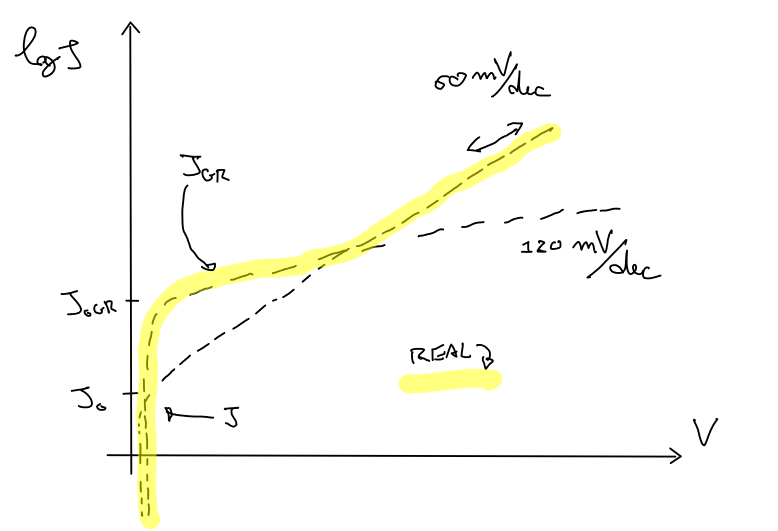
\includegraphics[width=0.5\textwidth]{lowcurrent.png}\\
\raggedright

Similar to ideal but $J_{0GR}$ is bigger and we have a factor 2 at the exp so there is a slight difference at very low current.

\centering
\fbox{\begin{minipage}{40em}
Note that $J_{0GR}\propto 1/\tau_0$ so is very process dependent and also that $J_{0GR}\propto n_i$ linear dependance on $n_i$ (wrt $J_0\propto n_i^2$) so at high temperature we recover the ideal diode characteristic.
\end{minipage}}
\raggedright

With reverse bias the current is dominated by $J_{RG}$ and have a slight increase due to the dependence of $W_d$ with V.\\

\centering
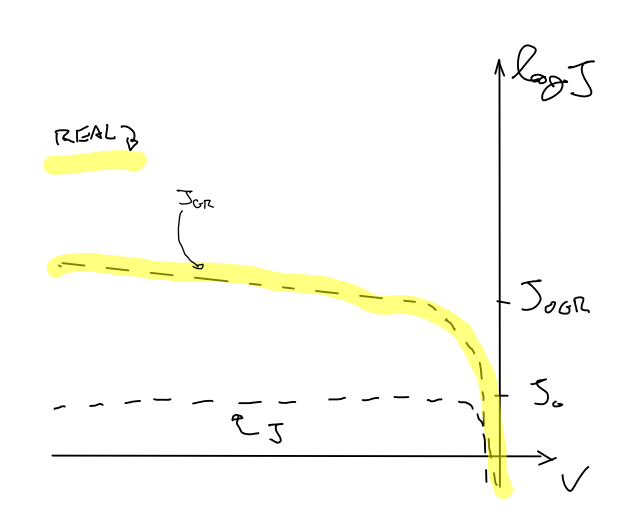
\includegraphics[width=0.35\textwidth]{inverselow.png}\\
\raggedright

\subsection{High current regime}
At high current regime there are 2 problems that create distortions in the ideal characteristic.\\
\vspace{5mm}
{\bf High injection regime}\\
At high current the hypotesis of low injection regime decades so taking p quasi-neutral region we have $n=n_0+\Delta n\simeq\Delta n$ and $p=p_0+\Delta n\simeq \Delta n$ so with the law of mass action generalized we obtain $pn=n_i^2e^{\frac{qV}{kT}}=\Delta n^2$ and so $\Delta n=n_ie^{\frac{qV}{2kT}}$ from this through continuity equation (see ~\ref{cont.eq}) we get that 
\begin{equation}
J\propto n_ie^{\frac{qV}{2kT}}
\end{equation}
so an additional solpe of 120mv/dec.\\ 
\vspace{5mm}
{\bf Resistive drops}\\
$E_f$ gradient is no more negligible so we have parasitic resistance due to the law $J_n=n\mu_n \frac{dE_{fn}}{dx}$.\\
To introduce this non ideality we can say that $J=J_0e^{\frac{qv}{mkT}}$ where m is a factor of non ideality.\\
What it follows is the Gummel plot of the pn junction that include all non idealities.\\

\centering
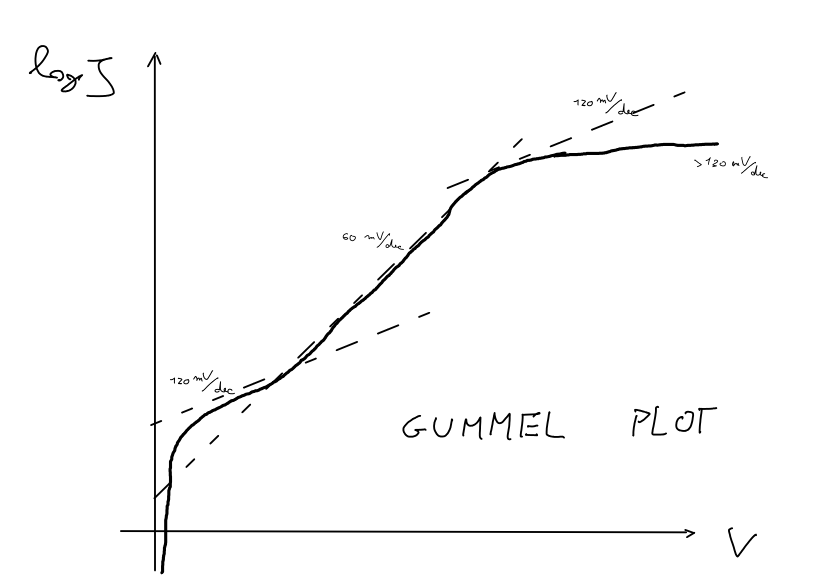
\includegraphics[width=0.5\textwidth]{gummel.png}\\
\raggedright

%------------------------------------------------------------------------%
\section{Small signal model}
%------------------------------------------------------------------------%
The pn junction is, of course, a non linear device if we assume that is polarized at $\overline{V}>0$ and we change that voltage of $\delta V$ we are interested in its response. We have 3 small signal parameters: conductance, depletion capacitance and diffusion capacitance.
%------------------------------------------------------------------------%
\subsection{Conductance}
Changing the voltage of $\delta V$ we have a variation of the current so a condctance that we can calculate as 
\begin{equation}
g_m=\frac{\partial I}{\partial V}=\frac{I}{kt/q}
\end{equation}
%------------------------------------------------------------------------%
\subsection{Deplition capacitance}
Changing $\delta V$ we remove a part of the depletion region as a consequence of majority injected in the junction that neutralize the fixed charges in the DL. We have a variation of the charge stored in the device as a consequence of a variation of the voltage so a capacitance.\\
We can introduce 
\begin{equation}
C_{dep}=\frac{\partial Q_{DL}}{\partial V}=-\frac{\partial }{\partial V}(qN_dx_n)=\frac{\varepsilon_{si}}{W_d}
\end{equation}
The minus sign is place in order to have a positive C and this formula is valid also for non constant doping concentration.\\
%------------------------------------------------------------------------%
\subsection{Diffusion capacitance}
Also in the quasi-neutral region we have charges stored that change if $\delta V$ change due to the excess of minority. This capacitance is called diffusion capacitance and is defined as 
\begin{equation}
C_{diff}=\frac{\partial Q_{diff}}{\partial V}
\end{equation} 
we have therefore define $Q_{diff}$. Assuming forward bias and so neglecting $n_{p0}$ we can write $Q_{diff}=\int^{W_p}_0 q\Delta n(x) dx$.\\
For a wide base diode we have 
\begin{equation}
Q_{diff}=q\Delta n(0) \frac{L_n^2}{L_n}\frac{D_n}{D_n}=J_n\tau_n
\end{equation}
For a narrow base diode 
\begin{equation}
Q_{diff}=q\Delta n(0) \frac{W_p^2}{2W_p}\frac{D_n}{D_n}=J_nt_p
\end{equation}
where $t_p=\frac{W_p^2}{2D_n}$ is defined as electron transit time through the quasi-neutral p region.\\

It's called like this beacuse from the current equation we can derive that $J_n=qD_n\Delta n(0)/W_p=q\Delta n(x) v_{diff}=q\Delta n(0)\frac{W_p-x}{W_p} v_{diff}$ from this we obtain $v_{diff}=\frac{D_n}{W_p-x}$ and from this integrating from 0 to $W_p$ in dx $\frac{1}{v_{diff}}$ we obtain exactly $t_p=\frac{W_p^2}{2D_n}$.\\
\vspace{5mm}
We could have come to the same result by reasoning on the physical situation: in the case of a wide-base diode, since we are in a stationary situation the amount of charge stored in the p-region cannot change, therefore if electrons are entering our region at a given rate, we must remove the same quantity at the same time, which is what the founded relation is saying
\begin{equation}
\frac{Q_{diff}}{\tau_0}=J_n
\end{equation}
Similarly, in a narrow-base diode the electrons entering the region must
recombine once they have reached the contact, therefore
\begin{equation}
\frac{Q_{diff}}{t_p}=J_n
\end{equation}
\vspace{5mm}\\

Going back to the diffusion capacitance we have for a wide base diode
\begin{equation}
C_{diff}^{wide}=g_m\tau_n
\end{equation} 
and for a narrow base
\begin{equation}
C_{diff}^{narrow}=g_mt_p
\end{equation}
In the end the small signal model is showed in figure.\\

\centering
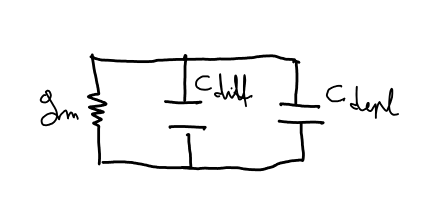
\includegraphics[width=0.35\textwidth]{smallpn.png}\\
\raggedright

In reverse bias the modulation of the quasi-neutral change is negligible and so is the diffusion capacitance.

        % Pn Junction
%------------------------------------------------------------------------%
%------------------------------------------------------------------------%
\chapter{Metal-semiconductor junction}
%------------------------------------------------------------------------%
Metal-semiconductor junctions can be divided in 2 categories: ohmic contacts ,that are what we've called "a good contact", and rectifing devices ,that work like diodes. A good contact is a low parasitic resistance device with 2 pin through wich can flow a lot of J with a small V. Rectifing devices let current flow only in one direction, for this type of device is needed a low doped semiconductor and a metal with a proper work function; this type of devices are called Schottky diodes.

%------------------------------------------------------------------------%
\section{Schottky diode}
%------------------------------------------------------------------------%
We will study the electrostatic of this device as we've done with diodes. We initially suppose the 2 zones isolated and under thermodinamic equilibrium. Let's take the semiconductor n-doped.\\
For the metal we're not interested in the conduction or valence band but only in the position of the Fermi level. All type of material's bands are refered to the vacuum level. The distance between the Fermi-level of the metal and the vacuum level $E_0$ is calle work-function $\phi_m$. For silicon we can define the electron affinity that is the distance between the conduction band and the vacuum level $\chi_s$. In this way we can allign the two materials like in figure.\\

\begin{wrapfigure}{i}{0pt}
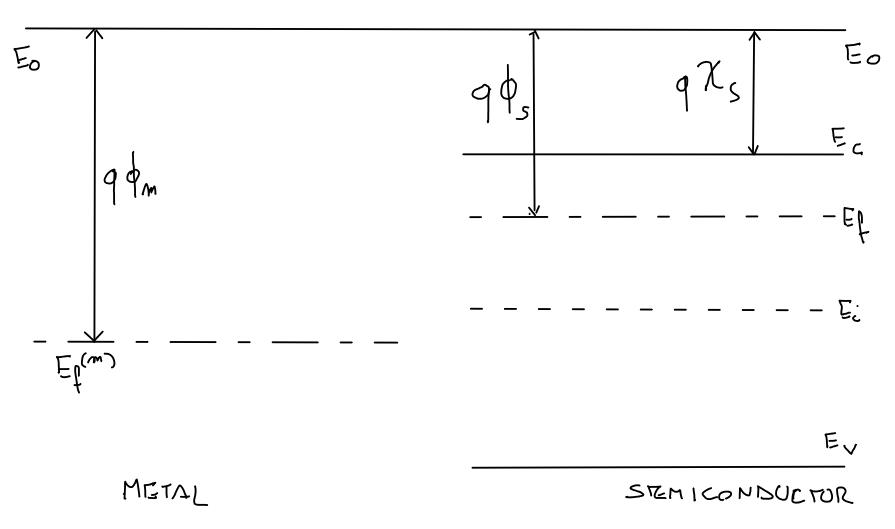
\includegraphics[width=0.5\textwidth]{ms1.png}
\end{wrapfigure}

Requirement for a Schottky diode are $E_f^{(m)}<E_f^{(s)}$ and a low doped semicondctor.\\
If we put the 2 materials toghether the distance between the difference $q\phi_m-q\chi_s=q\phi_{bn}$ is preserved in the semiconductor the bands goes up to align $E_f$ and we therefore have a built in potential $\phi_{bi}$. There is a diffusion process from semiconductor to metal and not in the opposite direction beacuse electrons of metal don't have enough energy.\\

\centering
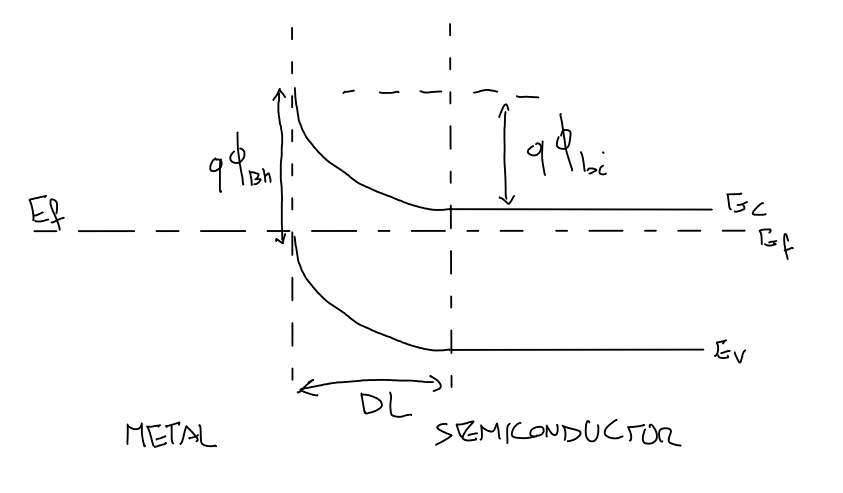
\includegraphics[width=0.5\textwidth]{ms2.png}\\
\raggedright
  
We can olso draw a graph of the electric field where we can view the deplition layer and the built in potential as area.\\
This device is an ideal unilateral $p^+-n$ junction; we have the depliton layer only in the n side. We can recove the expression from the diode   
\begin{equation}
W_d=\sqrt{\frac{2\varepsilon_{si}}{q}\frac{1}{N_d}\phi_{bi}}=x
\end{equation}  

\centering
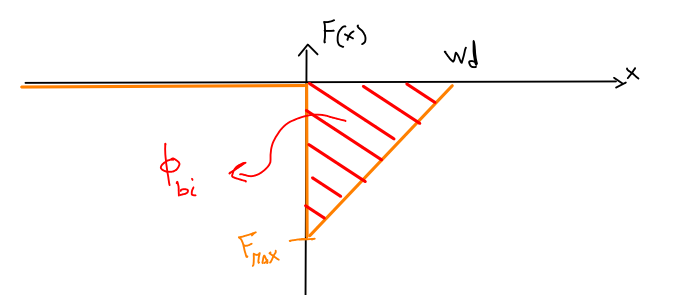
\includegraphics[width=0.5\textwidth]{ms3.png}\\
\raggedright

\subsection{Bias}
We will always consider the semiconductor part of the device n-doped and grounded; a voltage will be applied to the metal. As for the pn junction we consider foward bias if the voltage applied is grater than 0 and reverse bias if the voltage applied is less than zero.\\


\centering
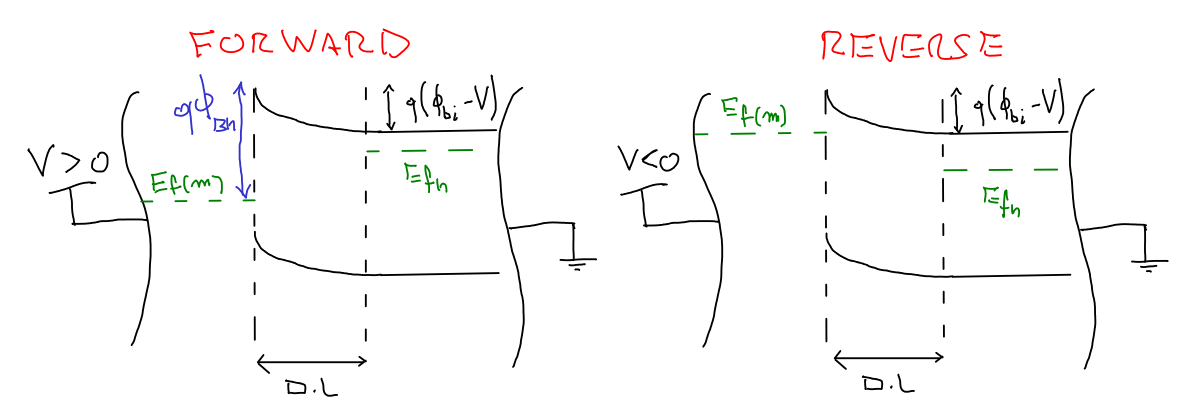
\includegraphics[width=0.55\textwidth]{msbias.png}\\
\raggedright


{\bf Reverse bias}\\
With reverse bias $E_{f(m)}$ becomes higher the depletion layer increases as the total voltage drop over the device.\\ 
{\bf Foward bias}\\
With foward bias $E_{f(m)}$ becomes lower, far from the contact we will have in the semiconductor a quasi-neutral region ,near the contact a transition zone with a depletion region. The total voltage drop decreases as the width of the depletion region.\\
We have two major difference with the pn junction: the flow of electrons from the semiconductor to the metal  don't have a minority constrain (the metal is full of electrons) so we will expect a high current but the transport of holes from metal to semiconductor has this limitation (the semiconductor is n-doped). $J_p$ will be small, negligible with respect to electrons flow.\\
Metal-semiconductor junction is a majority carrier device we won't deal with minority carrier in current transport phenomena. We will always neglect G-R processes beacuse are relevant only at low current regime.\\
%------------------------------------------------------------------------%
\subsection{Schottcky model}
%------------------------------------------------------------------------%
\centering
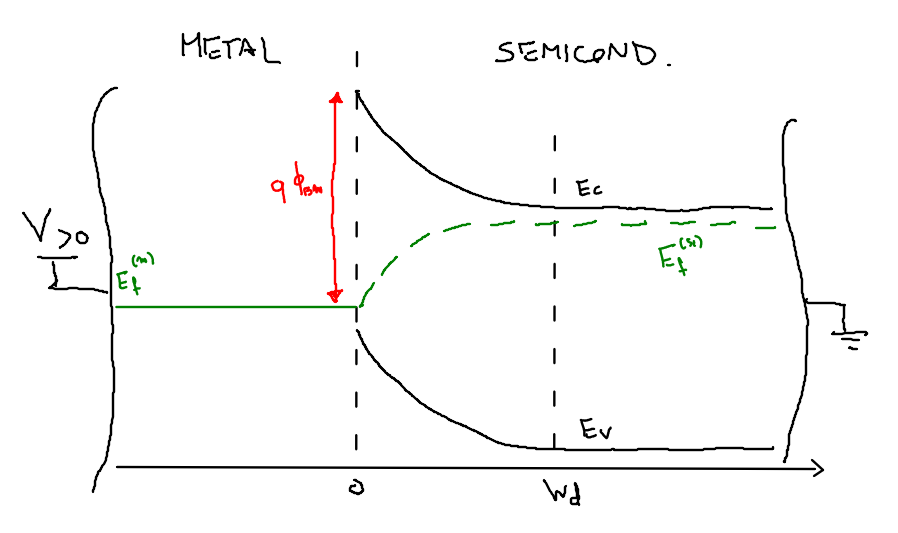
\includegraphics[width=0.45\textwidth]{shk.png}\\
\raggedright

We don't know the behaviour of $E_{fn}$ in the depletion layer but we know that in that zone we have the lower concetration of electrons so it can't be flat. Under stationary condition we can say that $ J_n=qn\mu_nF+qD_n \frac{dn}{dx}=$ constant and, as boundary condition, that $n(W_d)=N_d$ $n(0)=N_ce^{\frac{q\phi_{bn}}{kT}}$. F is given the only parameter we don't know is n and $\frac{dn}{dx}$ so solving the continuity equation for electrons with this boundary conditions we can get that
\begin{equation}
J=J_0(e^{\frac{qV}{kT}}-1)
\end{equation}
that is a relation identical to the pn junction but with a different $J_0$.\\
However this relation does not mach the experimental results. This is due to an implicit assumption that we've made using $n(0)=N_ce^{\frac{q\phi_{bn}}{kT}}$ as boundary condition; this happens only if the interface is always at thermodynamic equilibrium.\\
This model is valid for low mobility semicondutors (not for Si, Ge and GaAs).\\
%------------------------------------------------------------------------%
\subsection{Bethe's model}
%------------------------------------------------------------------------%
\begin{wrapfigure}{i}{0pt}
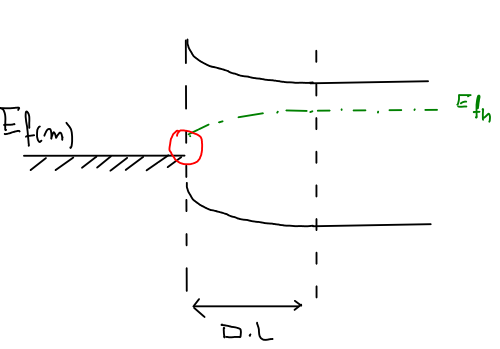
\includegraphics[width=0.25\textwidth]{msne.png}
\end{wrapfigure}

$E_{fn}$ can arrive at the interfae higher than $E_{f(m)}$. We have a very thin interface that is of the order of fractions of nm there we can't describe current transport with drift and diffusion theory beacuse they're dominated by scattering events that occurs in tens of nanometers. We have to use a thermoionc transport model.\\
The electrons that pass from semiconductor to metal are that with an energy greater than $q(\phi_{bi}-V)$ so an energy higher than the potential barier of the depletion layer.\\
From energy dispersion relation $E=E_c+\frac{\hslash^2k^2}{2m_x}+\frac{\hslash^2k^2}{2m_y}+\frac{\hslash^2k^2}{2m_z}$ we define $E_x=\frac{\hslash^2k^2}{2m_x}$ the energy related to x transport and let's take into account only one ellipsoide.\\

\begin{wrapfigure}{i}{0pt}
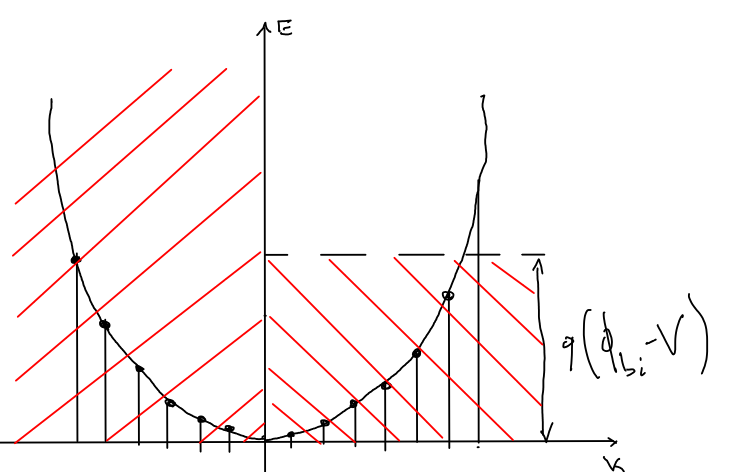
\includegraphics[width=0.25\textwidth]{bethe.png}
\end{wrapfigure}

Refering to the interface between the depletion layer and the quasi neutral region, half of the $E_x$ parabola can be neglected beacuse we want electrons that move from right to left (semiconductor to metal). We want olso to consider only electrons with energy higher than $q(\phi_{bi}-V)$ so with a $k_x>\overline{k}$ so we can neglect other states.\\
The equivalent current of this electrons will be 
\begin{equation}
J_{s-m}^{(1)}=\sum_{k_x>\overline{k}}2 \frac{q}{L^3}v_x(k_x)f(k_x,k_y,k_z)
\end{equation}
the 2 factor is a spin correction. Adding a corrective term we can transform the summation into an integral 
\begin{equation}
J_{s-m}^{(1)}=\frac{1}{(\frac{2\pi}{L})^3}\int_{\overline{k_x}}^{+\infty}\int_{-\infty}^{+\infty}\int_{-\infty}^{+\infty}\frac{q}{L^3}v_x(k_x)f(k_x,k_y,k_z)dk_xdk_ydk_z
\end{equation}
remembering that $\hslash k_{x,y,z}=m_{x,y,z}v_{x,y,z}$ therefore $dk_{x,y,z}=\frac{m_{x,y,z}}{\hslash}dv_{x,y,z}$, we can change integration variable as 
\begin{equation}
J_{s-m}^{(1)}=\frac{2q}{(2\pi)^3}\int^{+\infty}_{v_x}\int_{-\infty}^{+\infty}\int_{-\infty}^{+\infty}v_xf(k_x,k_y,k_z) \frac{m_xm_ym_z}{\hslash^3} dv_xdv_ydv_z
\end{equation}
for f we can use M-B approximation $f\simeq e^{-\frac{E-E_f}{kT}}$ using energy dispersion relation 
\begin{equation}
E=E_c+\frac{1}{2}m_xv_x+\frac{1}{2}m_yv_y+\frac{1}{2}m_zv_z
\end{equation}
the M-B equation becomes
\begin{equation}
f\simeq e^{-\frac{E_c-E_{fn}}{kT}}\cdot e^{-1/2\frac{m_xv_x^2}{kT}}\cdot e^{-1/2\frac{m_yv_y^2}{kT}}\cdot e^{-1/2\frac{m_zv_z^2}{kT}}
\end{equation}
so solving the 3 integral (the first is a gaussian $=\frac{kT}{m_x}e^{-\frac{m_xv_x^2}{kT}}$ second and third $=\sqrt{\frac{2kT\pi}{m_{y,z}}}$) we get 
\begin{equation}
J_{s-m}^{(1)}=\frac{4\pi q}{h^3}\sqrt{m_xm_y}(kT)^2e^{\frac{-\phi_{bn}}{kT}}e^{\frac{qV}{kT}}=A\cdot\sqrt{m_xm_y}T^2e^{\frac{-\phi_{bn}}{kT}}e^{\frac{qV}{kT}}
\end{equation}
where $A=\frac{4\pi qk^2}{h^3}=120 \frac{A^2}{cm^2 K^2}$ it's called the Richardson constant.\\

\begin{wrapfigure}{i}{0pt}
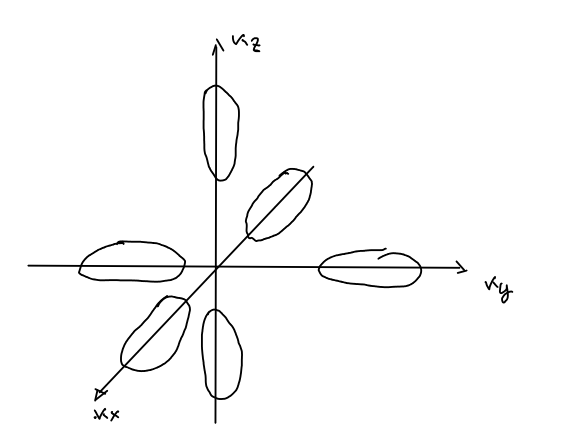
\includegraphics[width=0.2\textwidth]{ellips.png}
\end{wrapfigure}

Taking into account all the ellipsoide we get
\begin{equation}
J_{s-m}=A \frac{2m_t+4\sqrt{m_tm_l}}{m_0}T^2e^{\frac{-\phi_{bn}}{kT}}e^{\frac{qV}{kT}}=A^*T^2e^{\frac{-\phi_{bn}}{kT}}e^{\frac{qV}{kT}}
\end{equation}
with $A^*=A\cdot2.05$.\\
From m-s we can say that under th.eq the 2 current must be equal and that the barrier is costant equal to $q\phi_{bn}$ so $J_{m-s}=A^*T^2e^{\frac{-\phi_{bn}}{kT}}$.\\
So finally the total current throught the device will be 
\begin{equation}
J=A^*T^2e^{\frac{-q\phi_{bn}}{kT}}(e^{\frac{qV}{kT}}-1)=J_{0,th}(e^{\frac{qV}{kT}}-1)
\end{equation}
$\phi_{bn}$ it's a crucial parameter for current flow in metal semiconductor junction. We have a $J_{0,th}\simeq10^5 A/cm^2$ orders of magnitude higher with respect to the pn junction and a turn on voltage of 0.3-0.4 V.\\
This model is valid for high mobility semiconductors.\\
%------------------------------------------------------------------------%
\subsection{Universal model}
%------------------------------------------------------------------------%
We can connect the two models in an universal one.\\
Starting from Schottcky model we can use his assumption of $ J_n=qn\mu_nF+qD_n \frac{dn}{dx}=const$ and $n(W_d)=N_d$ but we have to change n(0). We can say something about $J_n(0)$ as the current density without scattering.

\begin{wrapfigure}{i}{0pt}
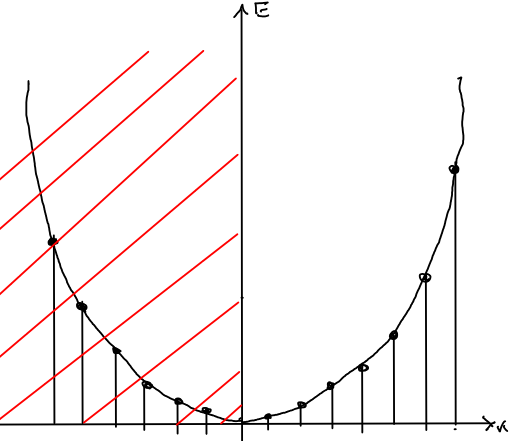
\includegraphics[width=0.2\textwidth]{generalmsmodel.png}
\end{wrapfigure}
 
We can calculate that term using energy dispersion relation but beacuse we are at the interface we will take all the left state of the parabola (we don't have a barrier) so we get 
\begin{equation}
J_n(0)=A^*T^2e^{-\frac{E_c-E_{fn}(0)}{kT}} 
\end{equation}
that is the correct boundary condition. If we muliply and divide this expression by $N_c$ we obtain
\begin{equation}
J_n(0)=A^*T^2 \frac{n(0)}{N_c}
\end{equation}
this for the electron flow from semiconductor to the metal. For the opposite direction we use the th.eq. condition and we get
\begin{equation}
J_n(0)=A^*T^2 \frac{n_0}{N_c}
\end{equation}
with $n_0$ electron concentration at the interface under th.eq.\\
So the final boundary condition is
\begin{equation}
J_n(0)=\frac{A^*T^2 }{N_c}[n(0)-n_0]
\end{equation}
We are using a drift-diffusion approach with thermionic boundary condition.\\
Solving this system we get an expression valid for all semiconductors that can be simplified in the 2 models depending on what type of semiconductor we have.\\
If mobility is large than it's easy to move electrons but difficult to remove them form the interface that becomes the bottom neck of the system. With low mobility it's difficult to move electrons but easy to remove them form the interfece so they don't pile up there.\\
%------------------------------------------------------------------------%
\subsection{Schottky effect}
%------------------------------------------------------------------------%
\begin{wrapfigure}{i}{0pt}
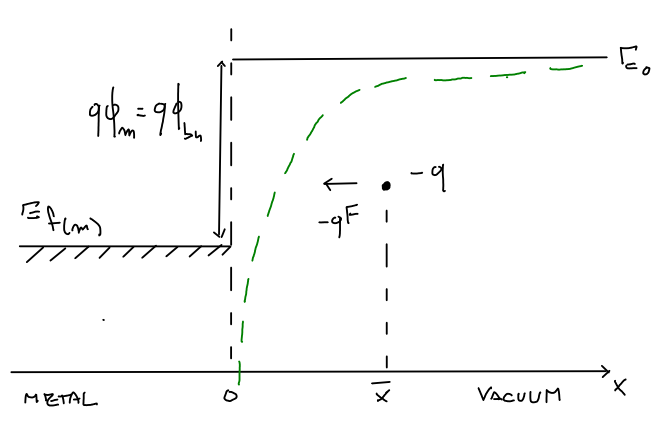
\includegraphics[width=0.4\textwidth]{scheff.png}
\end{wrapfigure}

The Schottky effect is a pure electrostatic effect that take place in the Bethe's model.\\
To study this effect we start from a metal-vacuum "junction" placing in the vacuum a single electron at a certain distance $\overline{x}$.\\
We have an electrostatic induction at the surface of the metal that attracts the electron in the vacuum near the surface. In order to calculate the electric field that attracts the single electron we can use the image method placing a positive charge +q at $-\overline{x}$ and removing the metal.\\
From this assumption we get 
\begin{equation}
-qF=\frac{1}{4\pi \varepsilon_0} \frac{-q^2}{(2\overline{x})^2}
\end{equation}
and so the electric field 
\begin{equation}
F=\frac{q}{16\pi\varepsilon_0x^2}
\end{equation}
from witch we can calculate ,integrating both part of the equation from x to $+\infty$, the potential as
\begin{equation}
\phi(x)=\phi(+\infty)+\frac{q}{16\pi \varepsilon_0 x}
\end{equation}
Multipling for -q we can obtain the energy 
\begin{equation}
E_0(x)=E_0(+\infty)-\frac{q^2}{16 \pi \varepsilon_0 x}
\end{equation}
and so the profile in green in the graph.\\

\centering
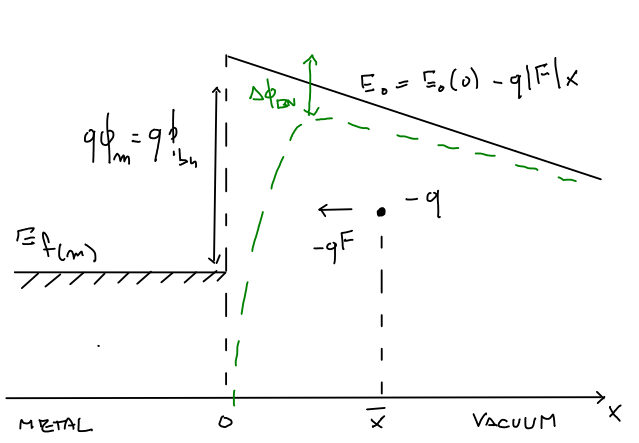
\includegraphics[width=0.35\textwidth]{deltaphibn.png}\\
\raggedright

If we consider that in the vacuum there is a costant electric field (and so $E_0(x)=E_0(0)-q|F|x$) like in figure beacuse the sistem is linear we obtain that
\begin{equation}
E_0(x)=E_0(0)-q|F|x-\frac{q^2}{16 \pi \varepsilon_0 x}
\end{equation}
and the behaviour in green in figure. We have change of the peak and so of the barrier that block our electrons. The $\Delta$ of the barrier is called Schottky barrier lowering.\\
We can calculate the new peak deriving by dx the $E_0(x)$ function finding the $x_{max}$ obtaining the energy at that point 
\begin{equation}
E_0(x_{max})=E_0(0)-\sqrt{\frac{q^3|F|}{4\pi \varepsilon_0}}
\end{equation}
So the difference in the barrier is $\Delta\phi_{bn}=\sqrt{\frac{q^3|F|}{4\pi \varepsilon_0}}$.\\
Now let's apply this effect on our metal semiconductor junction: when an electron travels throught the depletion layer from the semiconductor to the metal we have a barrier lowering of $\Delta\phi_{bn}=\sqrt{\frac{q^3|F_{max}|}{4\pi \varepsilon_{Si}}}$ (we place $F_{max}$ beacuse the maximum effect we have is with the max F and the narrower distance).\\
In our device we have a change of the J-V characteristic 
\begin{equation}
J=A^*T^2e^{\frac{-q(\phi_{bn}-\Delta\phi_{bn})}{kT}}(e^{\frac{qV}{kT}}-1)
\end{equation}
that creates an increment of $J_0$ and 2 opposit behaviour for reverse and forward bias: with $V<0$ the current increases increasing $|V|$, with $V>0$ J decrease this due to the dependance of $\Delta\phi_{bn}\propto\sqrt{F_{max}}\propto V_{rv-bias}$.\\
%------------------------------------------------------------------------%
\section{Ohmic contact}
%------------------------------------------------------------------------%
\begin{wrapfigure}{i}{0pt}
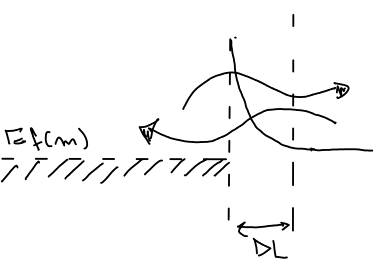
\includegraphics[width=0.15\textwidth]{tunnel.png}
\end{wrapfigure}

In order to have an ohmic contact we need a high doped semiconductor. With $N_d$ very high the depletion layer becomes narrower and increasing the doping concentration we arrive at a condition when there is a strong factor of J due to quantum-mechanical tunneling. That process does not depend on the type of bias so we don't have anymore a rectifing behaviour.\\

\centering
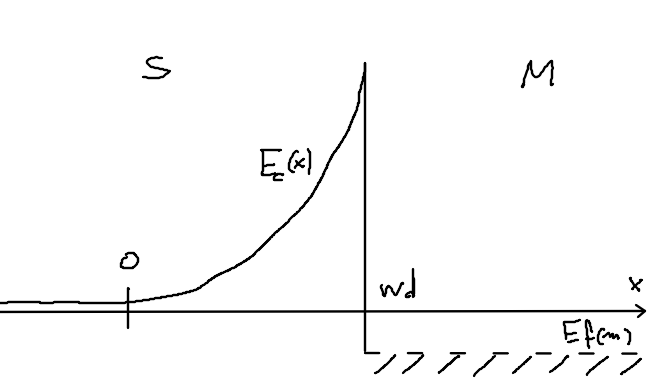
\includegraphics[width=0.35\textwidth]{1tunnel.png}\\
\raggedright

Taking into account the figure as reference system from the studied pn junction we know the behaviour of $E_c(x)=\frac{q^2N_d}{2\varepsilon_{Si}}x^2$ so we can calculate T ,transparancy coefficient as 
\begin{equation}
T=e^{-2\int Im\{E_c(x)\}dx}=e^{-2\int \sqrt{\frac{2m^*(E_c-E)}{\hslash^2}}dx}
\end{equation}
we have to remember that in this case $m^*$ is the effective mass for tunneling process. So if we consider $E=E_f$
\begin{equation}
T=e^{-2\int \sqrt{\frac{2m^*E_c}{\hslash^2}}dx}=e^{-2\sqrt{\frac{2m^*}{\hslash^2}}\sqrt{\frac{q^2N_d}{2\varepsilon_{Si}}}W_d^2/2}
\end{equation}
That substituiting $W_d$ with its expession we get
\begin{equation}
T=e^{-2\sqrt{\frac{2m^*}{\hslash^2}}\sqrt{\frac{q^2N_d}{2\varepsilon_{Si}}}\frac{2\varepsilon_{Si}}{qN_d}(\phi_{bi}-V)}=e^{-q \frac{(\phi_{bi}-V)}{E_{00}}}
\end{equation}
where $E_{00}=q\frac{\hslash \sqrt{N_d}}{2\sqrt{m^*\varepsilon_{si}}}$\\

\begin{wrapfigure}{i}{0pt}
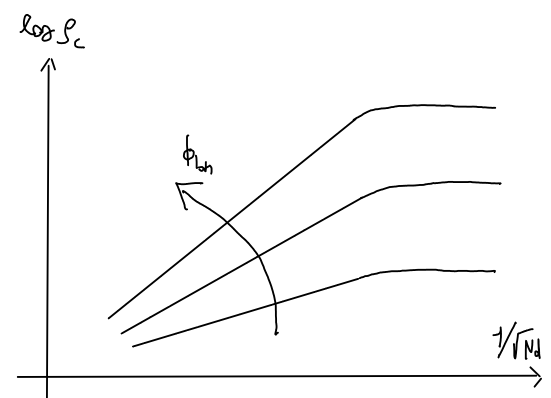
\includegraphics[width=0.3\textwidth]{contactrho.png}
\end{wrapfigure}

One important parameter of this device is the contact resistivity defined as 
\begin{equation}
\rho_c=(\frac{\partial J }{\partial V})^{-1}|_{V=0}=\frac{E_{00}}{q}e^{q\phi_{bi}/E_{00}}
\end{equation}
This parameter depends on the barrier hight and on $\sqrt{N_d}$. In the graph shows the $\log (\rho_c) - 1/\sqrt{N_d}$ dependance. It's a straight line until the concentration becomes too low and so tunneling effect is no more relevant.\\
To achive large current flow we need to perturbe only al little bit the device so it stays always near thermodynamic equilibrium.\\
The two figures below show how a contact is done in a device.

\centering
\includegraphics[width=0.5\textwidth]{ohmicconctact.png}\\
\raggedright

%------------------------------------------------------------------------%
\section{Interface states}
%------------------------------------------------------------------------%
We've always considered Si as a periodic infinite cristal but in metal-semiconductor junction we have te interface that interrupts the sequence of atoms. Some atoms of Si can't share all theyr 4 valence electrons creating some dangling bonds.\\

\begin{wrapfigure}{i}{0pt}
\includegraphics[width=0.3\textwidth]{is01.png}
\end{wrapfigure}

Electrons remains localize close to theyr silicon atoms this creates spurius energy level at the interface.\\ 
In the bulk region electrons and holes are only in the conduction band or in the valence band but at the interface can stay in a lot of states between this two bands.\\
The spurious states in the upper part of the bandgap have an acceptor behaviour (negativly charged when empty and neutral when filled) the others in the bottom part have a donor behaviour (neutral when filled and positivly charged when empty). The energy that divide this two type of states is the $E_{is}$.\\
All states above $E_f$ will be filled all the other states empty. So the previous band-diagram is incoherent with the Gauss'law since we have some exposed charge and no band banding.\\ 

\begin{wrapfigure}{i}{0pt}
\includegraphics[width=0.19\textwidth]{is02.png}
\end{wrapfigure}

We have a negative charge so $\phi<0$ the bands band upward and the distance $E_f-E_{is}$ becomes narrower. The bands banding create a depletion region that expose a positive charge equal to the interface states' charge.\\
The distance between $E_c-E_f$ is not set only by doping concentration but olso from interface states.\\
We define interface state density $N_{is} = [cm^{-2}eV^{-1}]$ in order to find the total charge introduced by the interface 
\begin{equation}
|Q_{is}|=N_{is}(E_f-E_{is})q
\end{equation}
The distance $E_c(0)-E_{is}\simeq E_{gap}/2$ so writing $\Delta E_{is}=E_c(0)-E_{is}\simeq E_{gap}/2$ we can say that
\begin{equation}
|Q_{is}|=N_{is}[\Delta E_{is}-(E_c(0)-E_{f})]q
\end{equation}
We know from the analysis of the pn junction that the charge in the depletion leyer is 
\begin{equation}
Q_{dep}=qN_dW_d=\sqrt{2\varepsilon_{si}qN_d\frac{E_c(0)-E_c(W_d)}{q}}
\end{equation}
where the last term is the voltage drop in the depletion layer.\\
For Gauss law this 2 terms have to be equal so solving the equation we get the level of the conduction band at the interface 
\begin{equation}
E_c(0)=\Delta E_{is}+\frac{\varepsilon_{si}N_d}{q^2N^2_{is}}-\sqrt{(\frac{\varepsilon_{si}N_d}{q^2N^2_{is}})^2+\frac{2\varepsilon_{si}N_d}{q^2N^2_{is}}(\Delta E_{is}-E_c(W_d))}
\end{equation}
This effect changes the barrerier hight and so theflow of current throught the device. $\phi_{bn}$ becomes strongly dependent on $N_{is}$

\subsection{Limit cases}
Starting from the equation $|Q_{is}|=Q_{dep}$ we have 2 limit cases.\\
$N_{is}=0$ in this case $E_c(0)=E_c(W_d)$ so we don't have a band banding we restore the ideal case.\\
$N_{is}\rightarrow +\infty$ in this case we notice that the first term has to be finite and so $\Delta E_{is}-(E_c(0)-E_{is}$ has to be zero that means that $E_c(0)=E_f+\Delta E_{is}$. \\
This case means we are moving $E_{is}$ up to $E_f$ that is totally indipendent from doping concentration but depends only from the interface states. This condition is called "Fermi level pinning at the surface".\\

The plot of $E_c(0)-\log(N_{is})$ make a transition between $10^{12}-10^{13}$ as order of magnitude.

\centering
\includegraphics[width=0.35\textwidth]{is03.png}\\
\raggedright
















        % Metal-semiconductor Junction
%------------------------------------------------------------------------%
%------------------------------------------------------------------------%
\chapter{MOS capacitor}
%------------------------------------------------------------------------%
We start our analysis with a 1D device, we will consider the substrate a monocristal of constant p-doped silicon.\\
We will consider for oxide $SiO_{2}$ that has a high energy gap ($\simeq$8-9eV), a low concentration of free carriers, a large resistivity, a reasonably low concentration of spurious difect ($\simeq 10^{10}cm^{-3}$) but a low dialectric constant ($\simeq 3.9$).This last propriety is the cause why recently $SiO_2$ is being substituted with high-k materials.\\
In our analysis we will consider the dialectric ideal (this means we have to solve only the Poisson eq. for the electrostatic beacuse there will be no current flow) and as gate material a metal.\\

%------------------------------------------------------------------------%
\section{Working regimes}
%------------------------------------------------------------------------%11
\centering
\includegraphics[width=0.7\textwidth]{mos_separate_material.png}\\
\raggedright

We start considering the 3 material isolated from each other under th.eq.\\
We will refer $E_{f(m)}\simeq E_{c}^{Si}$. we have also to introduce the vacuum level and so electron affinity for oxide and silicon, metal work function, and silicon work function. From this data we can say that the metal we need is Al in order to mantain $E_{f(m)}\simeq E_{c}^{Si}$.\\
We also underlined in red the potential barrier created by the oxide for holes and electrons.\\

\begin{wrapfigure}{i}{0pt}
\includegraphics[width=0.5\textwidth]{mos_theq.png}
\end{wrapfigure}

We put the 3 materials in contact after a while we will have a single Fermi-level all over the device and we can say that far from the contact p-Si will be at equilibrium.\\
$E_{f(m)}$ will move downwards toghether with $E_c^{ox}$ since the distance $E_{f(m)}-E_c^{ox}$ is constant (material dependent) as $E_{gap}^{ox}$ .
We have discontinuity of F, for Gauss law $\varepsilon_{ox}F_{ox}=\varepsilon_{Si}F_{Si}$and since $\varepsilon_{Si}=11.7\ \ \varepsilon_{ox}=3.9$ we get $F_{ox}=3F_{Si}(0)$. We have a linear band banding in the oxide for the hp of idealty of the dialectric (no charge distribution inside) and a parabolic band banding (that means a linear F) in the Si.\\
We have 2 voltage drops over the silicon and over the metal that define $V_s+V_{ox}=\phi_{bi}$.
If we apply a $V>0$ at the gate we push $E_{f(m)}$ downwards creating a higher band banding both in oxide and silicon, this band banding will increase both $V_{ox}$ and $V_{s}$ so assuming that the bulk keeps th.eq we can write the following equation
\begin{equation}
V_{G}+\phi_{bi}=V_s+V_{ox}
\end{equation}
%------------------------------------------------------------------------%
\subsection{Flat band regime}
%------------------------------------------------------------------------%
\begin{wrapfigure}{i}{0pt}
\includegraphics[width=0.5\textwidth]{mos_vfb.png}
\end{wrapfigure}

If we apply $V_G=-\phi_{bi}$ from the previous equation we have that $V_s=V_{ox}=0$ and a separation $E_{f(m)}-E_{f(Si)}=qV_G$.\\
This is the so called Flat-band condition of the mos capacitor 
\begin{equation}
V_{FB}=-\phi_{bi}
\end{equation}
Is defined as the voltage to apply at the gate to have all bands flat.\\
now we can re-write the balance of voltages as
\begin{equation}
V_G-V_{FB}=V_s+V_{ox}
\end{equation}

$V_{fb}$ can be found considering complete ionization as
\begin{equation}
V_{FB}=\frac{kT}{q}\ln(\frac{N_a}{n_i})+\frac{E_g}{2}
\end{equation}
%------------------------------------------------------------------------%
\subsection{Accumulation regime}
%------------------------------------------------------------------------%
\centering
\includegraphics[width=0.5\textwidth]{mos_accum.png}\\
\raggedright


If $V_G<V_{FB}$ bands band upwards we have more holes concentration at the interface between Si-Ox than the doping concentration. \\
This is calle the accumulation regime.
%------------------------------------------------------------------------%
\subsection{Deplition regime} 
%------------------------------------------------------------------------%
\centering
\includegraphics[width=0.5\textwidth]{mos_depl.png}\\
\raggedright

With $V_G>V_{FB}$ we have in silicon a depletion region so we are in the depletion regime of the mos capacitor.
%------------------------------------------------------------------------%
\subsection{Weak inversion condition}
%------------------------------------------------------------------------%
\centering
\includegraphics[width=0.5\textwidth]{mos_weak.png}\\
\raggedright

If we further increase $V_G>>V_{FB}$ we arrive at the condition that the intrinsic Fermi level at the surface reaches the Fermi level ($E_f=E_i$).\\
From now on if we slightly increase the voltage we will have more electrons than holes at the interface. This is the condition for weak inversion condition.\\
%------------------------------------------------------------------------%
\subsection{Strong inversion regime}
%------------------------------------------------------------------------%
If we continue to increase the voltage applied we will reach the strong inverson regime that is characterized by $(E_i-E_f)|_{interface}=-(E_i-E_f)|_{bulk}$ so the concentration of electrons at the interface is equal to the doping concentration in the bulk.




%------------------------------------------------------------------------%
\section{Electrostatics}
%------------------------------------------------------------------------%
\centering
\includegraphics[width=0.5\textwidth]{mos_electrostatic.png}\\
\raggedright

We have to solve the Poisson equation $\frac{d^2\phi}{dx^2}=-\frac{q}{\varepsilon_{Si}}(p-n-N_a^-)$ only in the substrate.\\
We define $\phi_B=(E_f-E_i)_{bulk}/q=[E_f=0]=-\frac{kT}{q}\ln(N_a/n_i)$ the electrostatic potential of the bulk far away from the interface and we take $E_f$ that is costant as the reference energy level 0.\\
We introduce also $\Delta \phi (x)=\phi(x)-\phi_B$  that is the change of the electrostatic potential wrt the bulk;$\Delta \phi (W_d)=0$ and $\Delta \phi (0)=V_s$.\\
\vspace{5mm}
Now we have to write $p-n-N_a^-$ as function of $\phi(x)$.\\
For electrons we can say that $n=n_ie^{(E_f-E_i)/kT}$ if we multiply and divide by q we get $n=n_ie^{q\phi(x)/kT}$ same for holes as $p=n_ie^{-q\phi(x)/kT}$. Electrons and holes in the bulk are $n_0=n_ie^{q\phi_b/kT}$ and $p_0=n_ie^{-q\phi_b/kT}$. From this 4 equation we can write that 
\begin{equation}
n=n_0e^{q\Delta \phi/kT} \ \ \ \ \ \ \ \ p=p_0e^{-q\Delta \phi/kt}
\end{equation}
In the bulk we can say ythat $p_0=n_0+N_a$ so 
\begin{equation}
N_a=p_0-n_0
\end{equation}
Now Poisson equation becomes 
\begin{equation}
\frac{d^2\phi}{dx^2}=-\frac{q}{\varepsilon_{Si}}(p_0e^{-q\Delta \phi/kt}-n_0e^{q\Delta \phi/kT}-p_0+\frac{n_i^2}{p_0})
\end{equation}
Until now the only approximation we have made is the M-B. Now we consider the complete ionization approximation $p_0\simeq N_a$. And we make a change of variable 
\begin{equation}
\frac{d^2\phi}{dx^2}=-\frac{q}{\varepsilon_{Si}}(N_ae^{-q\Delta \phi/kt}-\frac{n_i^2}{N_a}e^{q\Delta \phi/kT}-N_a+\frac{n_i^2}{N_a})
\end{equation}
\begin{equation}
d(\frac{d\phi}{dx})=-\frac{q}{\varepsilon_{Si}}(N_ae^{-q\Delta \phi/kt}-\frac{n_i^2}{N_a}e^{q\Delta \phi/kT}-N_a+\frac{n_i^2}{N_a})dx
\end{equation}
\begin{equation}
\frac{d\phi}{dx}d(\frac{d\phi}{dx})=-\frac{q}{\varepsilon_{Si}}(N_ae^{-q\Delta \phi/kt}-\frac{n_i^2}{N_a}e^{q\Delta \phi/kT}-N_a+\frac{n_i^2}{N_a})dx\frac{d\phi}{dx}
\end{equation}
Now we integrate one time this expression form $\Delta \phi$ to 0. The first member is like f(x)f'(x) so the result is $-1/2(\frac{d\phi}{dx})^2$. Integrating also the second member and gathering the common terms the equation we get
\begin{equation}
(\frac{d\Delta \phi }{dx})^2=\frac{2kTN_a}{\varepsilon_{si}}\left(e^{-q\Delta \phi/kT}+\frac{q\Delta \phi}{kT}-1+\frac{n_i^2}{N_a^2}(e^{q\Delta \phi/kT}-\frac{q\Delta \phi}{kT}-1)\right)=F^2(x)
\end{equation}
For Gauss law $F(0)=-\frac{Q_s}{\varepsilon_{si}}$ (and also that $\Delta \phi (0)=V_s$ )from this relation and the previous equation we get
\begin{equation}
Q_s=\pm\sqrt{2kTN_a\varepsilon_{si}}\left(e^{-qV_s/kT}+\frac{qV_s}{kT}-1+\frac{n_i^2}{N_a^2}(e^{qV_s/kT}-\frac{qV_s}{kT}-1)\right)^{1/2}
\end{equation}
We already know the total charge in the substrate for all working regimes.\\
%------------------------------------------------------------------------%
\subsection{Dominant terms in the solution of Poisson equation}
%------------------------------------------------------------------------%
\centering
\includegraphics[width=0.5\textwidth]{logqVs.png}\\
\raggedright

To better undestand this formula let's analyse all working regime separately and draw a $\log |Q_s| - V_s$ graph.\\

\vspace{5mm}
In accumulation regime when $V_s<0$ we have that $Q_s\simeq \sqrt{2kTN_a\varepsilon_{si}}e^{-\frac{qV_s}{2kT}}$. So in the graph we see a straight line dependence. We can say that the term
\begin{equation}
e^{\frac{-qV_s}{kT}}\rightarrow h_{sub}
\end{equation} 
in the solution of the Poisson equation is the term that takes into account for hole concentration in the substrate.\\

\vspace{5mm}
In the depletion regime $0<V_s<2|\phi_b|$ we have to consider two dominant term: $\frac{qV_s}{kT}$ and $\frac{n_i^2}{N_a^2}e^{\frac{qV_s}{kT}}$. If we evaluate the second term at $2|\phi_b|$ we get 1 so it's negligible and therefore the first term is predominant. In this regime
\begin{equation}
Q_s\simeq -qN_a\sqrt{\frac{2\varepsilon_{Si}}{q}\frac{1}{N_a}V_s}=-qN_aW_d
\end{equation}
that is the charge of the depletion layer.\\

\vspace{5mm}
In strong inversion $Q_s\simeq \sqrt{2kTN_a\varepsilon_{si}}\frac{n_i}{N_a}e^{\frac{qV_s}{2kT}}$ so we can say that the term
\begin{equation}
\frac{n_i^2}{N_a^2}e^{\frac{qV_s}{kT}}\rightarrow e_{sub}
\end{equation}
in the solution of the Poisson equation is the term that takes into account electrons in the substrate.\\

%------------------------------------------------------------------------%
\subsection{Total charge in function of gate bias}
%------------------------------------------------------------------------%
We want $Q(V_g)$ not $Q(V_s)$; to have that expression we need to remember that $V_g-V_{fb}=V_s+V_{ox}$ but we can write $V_{ox}=F_{ox}t_{ox}=\frac{\varepsilon_{Si}F_{Si}}{\varepsilon_{ox}}t_{ox}=-Q(V_s)/C_{ox}$ so $V_g-V_{fb}=V_s-\frac{Q_s}{C_{ox}}$ using this expression and $Q_s=Q_s(V_s)$ we can get what we want.\\
We will plot also the 2 graphs $V_s-V_g$ and $|Q_s|-V_g$.\\

\centering
\includegraphics[width=0.5\textwidth]{qvs.png}\\
\raggedright


We will take as reference point the flat band condition where $Q_s=0$ and $V_s=0$.\\

\vspace{5mm}
For $V_s<0$ we said that  $Q_s\simeq \sqrt{2kTN_a\varepsilon_{si}}e^{-\frac{qV_s}{2kT}}$ so we get that
\begin{equation}
V_g-V_{fb}=V_s-\frac{\sqrt{2kTN_a\varepsilon_{si}}}{C_{ox}}e^{-\frac{qV_s}{2kT}}
\end{equation} 
we can neglect the first $V_s$ beacuse it's negligible wrt the exponential term so we get 
\begin{equation}
V_s\simeq-\frac{2kT}{q}\ln\left(\frac{C_{ox}(V_{fb}-V_g)}{\sqrt{2kTN_a\varepsilon_{si}}} \right) \ \ \ \ \ \ Q_s\simeq C_{ox}(V_{fb}-V_g)
\end{equation}
a small variation of $V_g$ let $V_s$ move not so much due to the exponential increase of the charge in the bulk and a consequent big field in the oxide; we are not far from a metal plate capacitor.\\

\vspace{5mm}
For $0<V_s<\phi_b$ we get that $Q_s\simeq \sqrt{2qN_a\varepsilon_{Si}V_s}$ so we get the following equation (that we don't solve)
\begin{equation}
V_g-V_{fb}=V_s+\frac{\sqrt{2qN_a\varepsilon_{Si}V_s}}{C_{ox}}
\end{equation}

\vspace{5mm}

{\begin{center} \fbox{\begin{minipage}{40em}

For weak inversion $\phi_b<V_s<2\phi_b$ we can consider both dominants terms 
getting the following equation 
\begin{equation}
V_g-V_{fb}=V_s+\frac{\sqrt{2\varepsilon_{si}kTN_a}}{C_{ox}}\left(\frac{qV_s}{kT}+\frac{n_i^2}{N_a^2}e^{qV_s/kT} \right)^{1/2}
\end{equation}
\begin{equation}
V_g-V_{fb}\simeq V_s+\frac{\sqrt{2\varepsilon_{si}kTN_a}}{C_{ox}}\sqrt{\frac{qV_s}{kT}}\left(1+\frac{n_i^2}{2N_a^2}e^{qV_s/kT}\frac{kT}{qV_s}\right)
\end{equation}
using Taylor expansion we get an exponential dependance on $V_g$ of the e charge (that is the second term). Form this dependace we will get the sub-th current of the mos capacitor.\

\end{minipage}}
\end{center}}



\vspace{5mm}
For strong inversion we get 
\begin{equation}
V_g-V_{fb}=V_s+\frac{\sqrt{2\varepsilon_{si}kTN_a}}{C_{ox}}\frac{n_i}{N_a}e^{qV_s/2kT}
\end{equation}
remembering that $\frac{n_i^2}{N_a^2}e^{q2|\phi_b|/kT}=1$ we can say that $\frac{n_i}{N_a}=e^{-q2|\phi_b|/2kT}$ so we can write that 
\begin{equation}
V_g-V_{fb}=V_s+\frac{\sqrt{2\varepsilon_{si}kTN_a}}{C_{ox}}e^{\frac{q(V_s-2|\phi_b|)}{2kT}}
\end{equation}
So we get $V_s$ 
\begin{equation}
V_s=2|\phi_b|+\frac{2kT}{q}\ln \left(\frac{C_{ox}(V_g-V_{fb}-V_s)}{\sqrt{2\varepsilon_{si}kTN_a}} \right) 
\end{equation}
and making a rought approx of $V_s\simeq 2|\phi_b|$, due to the log dependance, also $Q_s$\\
\begin{equation}
Q_s=-C_{ox}(V_g-V_{fb}-V_s)\simeq-C_{ox}(V_g-V_{fb}-2|\phi_b|)
\end{equation}
The approximation means that entering in storng inversion we get a maximum depletion layer and a maximum depletion charge
\begin{equation}
W_d^{max}=\sqrt{\frac{2\varepsilon_{si}}{qN_a}2|\phi_b|} \ \ \ \ \ \ \ \ \ Q_{dep}^{max}=-\sqrt{2\varepsilon_{si}qN_a2|\phi_b|}
\end{equation}
we increase the charge of electrons not that of the depletion layer.\\
The $V_g$ at witch we enter in the strong inversion is $V_g-V_{fb}=2|\phi_b|+\frac{|Q_{dep}^{max}|}{C_{ox}}$ that is called threshold voltage of the mos capacitor that is 
\begin{equation}
V_t=V_{fb}+2|\phi_b|+\frac{|Q_{dep}^{max}|}{C_{ox}} \ \ \ \rightarrow Q_{inv}=Q_s-Q_{dep}^{max}=-C_{ox}(V_g-V_t)
\end{equation}

%------------------------------------------------------------------------%
\section{Small signal capacitance}
%------------------------------------------------------------------------%
We want to study the small signal capacitance of the MOS capacitor that is a non linear device so we want $C_g=-\frac{dQ_s}{dV_g}$ the change of charge over the change of voltage.\\
We can guess the behaviour of $C_g$ using the expression $V_g-V_{fb}=V_s-Q_s/C_{ox}$ and calculating the derivative wrt $d(-Q_s)$ we get
\begin{equation}
\frac{dV_g}{d(-Q_s)}=\frac{dV_s}{d(-Q_s)}+\frac{1}{C_{ox}}
\end{equation}
that is 
\begin{equation}
\frac{1}{C_g}=\frac{1}{C_s}+\frac{1}{C_{ox}}
\end{equation}
The total gate capacitance can be expressed by the series of 2 capacitive terms one fixed ($C_{ox}$) one variable (that is the substrate capacitance $C_s$). From this we know that $C_g$ has an upper limit of $C_{ox}$.\\
Let's analise the small signal capacitance in the various regime.\\

\subsection{in accumulation regime}
We derivate the charge of the accumulation region obtaining 
\begin{equation}
C_s=\sqrt{2kTN_a\varepsilon_{si}}e^{-\frac{qV_s}{2kT}}\frac{q}{2kT}=Q_s/\frac{2kT}{q}
\end{equation}
Knowing $Q_s(V_g)$ we get 
\begin{equation}
C_s=\frac{C_{ox}(V_{fb}-V_g)}{2kT/q}
\end{equation}
This is $>>C_{ox}$ if $V_{fb}-V_g>>2kT/q$. So from flat band to minus infinite the capacitance increases and becomes similar to $C_{ox}$. We are close to a metal plate capacitor.\\

\subsection{in flat band condition}
We have to include in the Q expression both electrons and holes so $Q_s=\sqrt{2kTN_a\varepsilon_{si}}(e^{\frac{-qV_s}{kT}}+\frac{qV_s}{kT}-1)^{1/2}$.\\ If we make the Taylor expansion of the exponential term around 0 we get $Q_s=-V_s\sqrt{\frac{\varepsilon_{si}q^2N_a}{kT}}$ so 
\begin{equation}
C_s=\frac{d(-Q_s)}{dV_s}=\frac{\varepsilon_{si}}{\sqrt{\frac{\varepsilon_{si}kT}{q^2 N_a}}}=\frac{\varepsilon_{si}}{L_D}
\end{equation}
we can recognise the Dybae lenght in the expresison we can interpretate this result as this ; the holes (majority) screen a perturbation of the electric field form the gate like a step increase of doping concentration.\\
This capacitance and the oxide capacitance are comparable.\\

\subsection{in depletion regime}
In depletion regime we have a charge $Q_s=-\sqrt{2\varepsilon_{Si} q N_a V_s}$ that is the usual expression for the charge in a depletion layer. From the well known realtion $C=\varepsilon_{si}/W_d$ we get 
\begin{equation}
C_g=C_{ox}/\sqrt{1+2C_{ox}^2 \frac{V_g-V_{fb}}{\varepsilon_{si}qN_a}}
\end{equation}
This capacitance decrease quickly near the flat band condition beacuse the contribution related to holes disappears over a few kT/q.\\

\subsection{in strong inversion} 
We have the charge $Q_s=\sqrt{2\varepsilon_{Si}kTN_a}\frac{n_i}{N_a}e^{\frac{qV_s}{2kT}}$ so making the derivate we reach 
\begin{equation}
C_s=\frac{|Q_s|}{2kT/q}=C_{ox}\frac{(V_g-V_{fb}-2|\phi_b|)}{2kT/q}
\end{equation}
Increasing $V_g$ we get a larger capacitance we reach a condition similar to a metal plate capacitance.\\

\centering
\includegraphics[width=0.35\textwidth]{c-g1.png}\\
\raggedright



%------------------------------------------------------------------------%
\section{Frequency regimes}
%------------------------------------------------------------------------%
\centering
\includegraphics[width=0.7\textwidth]{c-gtot.png}\\
\raggedright

Let's look more colsely to the substrate during the different regimes when we apply a small signal to the gate.\\

\vspace{5mm}
{\bf In accumulation regime}\\
$\overline{V_g}<V_{fb}$ if we move the gate of $\delta V_g>0$ we are removing h from the silicon surface to the substrate. Vice-versa with $\delta V_g<0$ we move h from the substrate to the silicon surface.\\
This is a modulation of majority carriers concentration so it happens in a very short time in the order of the dialectric relaxation time.\\

\vspace{5mm}
{\bf In weak inversion}\\
$V_{fb}<\overline{V}<V_t$ we have a depletion region with a certain voltage drop $V_s$ and an exposed negative charge at the surface.\\
With a $\delta V_g>0$ we slightly increase the width of the depletion layer so we are removing holes from the edge of the depletion layer to the substrate. With $\delta V_g<0$ we reduce the depletion layer so we add h from the substrate to the depletion layer to neutralize the exposed charge.\\
Also here we modulate the majority carrier so this is a process that have as time constant the dialectric relaxation time.\\

\vspace{5mm}
{\bf Strong inversion}\\
Depletion layer at the maximum expansion at the silicon surface we have a lot of electrons.\\ 
Appling $\delta V_g$ we modulate e concetration this electrons cannot came from the contact that exchange only majority they have to be created by generation processes.\\

%------------------------------------------------------------------------%
\subsection{Low frequency regime}

\begin{wrapfigure}{i}{0pt}
\includegraphics[width=0.4\textwidth]{lfbd.png}
\end{wrapfigure}
The time constant for the generation process in strong inversion can be extracted from the generation current $J_g=q\frac{n_i}{2\tau_0}W_d^{max}$ that is the total current that can be created per unit time per unit area. The charge of the depletion layer is $Q_{dep}=qN_aW_d^{max}$ the time for generate this charge is 
\begin{equation}
\tau_g=\frac{Q_{dep}}{J_g}=2\tau_0N_a/n_i
\end{equation}
$\tau_g$ is technology dependent and very big in the order of seconds.\\
Only if the signal has a frequence much lower than $\tau_g$ ($f<1Hz$) we have the ideal charachteristic seen before.\\
Looking at the band diagram a movement of $\delta V_g$ moves $E_{f(m)}$ upwards or downwards. With a $\delta V_g>0$ we have to increase the total voltage drop but the dependance with $V_{sub}$ is very weak (logaritmic dependance) so $\delta V_s\simeq 0$ and we modulate only the voltage drop over the oxide (this under charge sheet approximation ,that we will see in next chapter, since we're  breaking the continuity law of the electric field $F_{ox}\varepsilon_{ox}=F_{Si}\varepsilon_{Si}$) $\delta V_g\simeq \delta V_{ox}$


%------------------------------------------------------------------------%
\subsection{High frequency regime}

\begin{wrapfigure}{i}{0pt}
\includegraphics[width=0.4\textwidth]{hfbd.png}
\end{wrapfigure}
For signals with high frequency ($f>1Hz$) we cannot change electron concentration so we can only add or remove holes at the substrate making the depletion layer bigger or smaller.\\ 
The graph of $C_g$ remains constant form the threshold voltage on.\\
The total capacitance depends on the frequency of the small signal we are appling.\\
Here the modulation of $\delta V_g$ can't modulate the electron concentration at the surface of silicon. There is a modulation of the depletion layer so $\delta V_s$ but for the continuity of the electric field also $\delta V_{ox}$ have to change in a comparable manner. With the downwards band banding we have to keep constant the distance with $E_{fn}$ with the conduction band so our substrate is no longer at th.eq. This triggers GR processes that tends to move the system back in the th.eq of low freqeuncy.
$E_{fn}$ is constant over the depletion layer and merges with $E_{fp}$ in the quasi neutral region of the device. We have a flow of electrons from the substrate to the surface similar to the pn-j reverse current.\\

%------------------------------------------------------------------------%
\subsection{Deep deplition}

\begin{wrapfigure}{i}{0pt}
\includegraphics[width=0.4\textwidth]{ddcond.png}
\end{wrapfigure}

If we consider a step increase of the gate voltage form 0 to $\overline{V}_g>V_t$ we don't give the time to the system to create electrons so we get a super wide depletion layer $W_d>>W_d^{max}$. This is called deep depletion condition of the MOS capacitor and it's a large signal regime.\\
If we apply on this step increase a $\delta V_g$ this will modulate the width of the depletion layer (in low and high freqence too) beacuse we don't have electron at the interface. The capacitance is $C_s=C_{dep}=\varepsilon_{si}/W_d$ so the total capacitance will decrease over V.\\
$W_d$ is related to $V_s$ so $W_d>W_d^{max}$ means $V_s>2|\phi_b|$ the conduction band can bend even below the fermi level but we have to keep the condition of no electrons at the interface so we have the split in the two Fermi level for electrons and holes. Small voltage drop over the oxide due to big voltage drop over the substrate.\\
GR processes will pull the system to the LF regime in order to restore the equilibrimu so with a $Q_{inv}$ of electrons at the surface.\\

\begin{wrapfigure}{i}{0pt}
\includegraphics[width=0.3\textwidth]{qinv.png}
\end{wrapfigure}

Let's study the behaviour in time of this charge under the simplifing assumption that $Q_s$ remains constant: so by S-R-H statisic 
\begin{equation}
\frac{dQ_{inv}}{dt}=-qG[W_d(t)-W_d^{max}]=-q \frac{n_i}{2\tau_0}[W_d(t)-W_d^{max}]
\end{equation}
but $Q_s=Q_{inv}+Q_{dep}=Q_{inv}-qN_aW_d(t)$ from here we get that $W_d(t)=(Q_{inv}-Q_s)/(qN_a)$ where $Q_s$ is a constant so we get the following differential equation
\begin{equation}
\frac{dQ_{inv}}{dt}=\frac{n_i}{2\tau_0N_a}Q_{inv}+\frac{qn_i}{2\tau_0}[\frac{Q_s}{qN_a}+W_d^{max}]
\end{equation}
that is a simple first order differential equation which solution is
\begin{equation}
Q_{inv}(t)=[Q_s+qN_aW_d^{max}][1-e^{t/t_g}] \ \ \ \ \ \ t_g=\frac{2\tau_0N_a}{n_i}
\end{equation}
so an exponential increase of the charge with a time constant $t_g$


%------------------------------------------------------------------------%
\section{MOS capacitor with ring}
%------------------------------------------------------------------------%
\centering
\includegraphics[width=0.7\textwidth]{ring.png}\\
\raggedright
We want to modify the structure adding a contact that can provide a lot of electrons. This contact is called ring it's $n^+$ doped. With $V_g>V_t$ $E_{fn}$ goes down but the Fermi level in the ring is higher than it so there is a flow of electrons from the ring to the substrate with a time constant similar to the transient time from the 2 zones of the electrons.\\

%------------------------------------------------------------------------%
\subsection{Split C-V curve}
\begin{wrapfigure}{i}{0pt}
\includegraphics[width=0.5\textwidth]{splitcv.png}
\end{wrapfigure}
With this structure it's possible to measure the current of electrons and holes indipendently and split the 2 contributions.\\
Let's assume that in accumulation regime and weak inversion we modulate only $dQ_p$ (no $dQ_n$ flow) so the capacitance is only $\frac{dQ_p}{dV_g}=C_g$ beacuse $\frac{dQ_n}{dV_g}=0$.
At stong inversion we modulate only electrons beacuse we reach the maximum width of the depletion layer so $\frac{dQ_p}{dV_g}=0$ and $\frac{dQ_n}{dV_g}=C_g$.\\ In this way we are splitting the total gate capacitance in 2 contributions due to holes and electrons.\\


%------------------------------------------------------------------------%
\subsection{Electrostatic}
%------------------------------------------------------------------------%
\centering
\includegraphics[width=0.35\textwidth]{sections.png}\\
\raggedright

Beacuse the MOS capacitor is an intrinsic 2D device we have to study the electrostatics in the 2 directions of the graph. \\ 
We are not intrested in polrization with $V_r<0$ beause this will make the pn junction in forward bias.\\



%------------------------------------------------------------------------%
\subsubsection{$\rightarrow V_r=V_g=0$}

\centering
\includegraphics[width=0.7\textwidth]{theqmosr.png}\\
\raggedright

We are under th.eq we are not perturbing the device. In crossection 1 we have weak inversion. In crossection 2 we have 1 single Fermi level for th.eq from crossection 1 we know the distance between the conduction band and $E_f$ in the substrate. The region under the gate in graph 2 is depleted


%------------------------------------------------------------------------%
\subsubsection{$\rightarrow V_r=0 \ \ \  V_g=V_t$}

\centering
\includegraphics[width=0.7\textwidth]{what1.png}\\
\raggedright

First graph is the one we have already seen. In crossection 2 we make the same consideration as before.


%------------------------------------------------------------------------%
\subsubsection{$\rightarrow V_r>0 \ \ \ V_g=0$}

\centering
\includegraphics[width=0.7\textwidth]{b1.png}\\
\raggedright

We have no change in the vertical crossection wrt the first case.
For the horizontal crossection we have to set the distance $E_c-E_f$ under the gate in accord to the first graph. In the $n^+$ region we are applying a potential that bands the band downwards by an amount $qV_r$ giving a large band banding and so a separation of the Fermi levels.\\
The quasi Fermi level for electrons has to stay constant for simmetry $E_{fp}$ changes.\\
Form this we have to modify graph 1 where $E_{fn}$ is moved downwards by an amount $qV_r$ (doing this we do not change the electrostatic beacuse the electron concetration was already negligible so no other modifications in the band banding are needed).\\

%------------------------------------------------------------------------%
\subsubsection{$\rightarrow V_r>0 \ \ \  V_g=V_t$}
Crossection 1 same as the case of $V_r=0 \ \ V_g=V_t$ with the same step of before we get the separation of the quasi Fermi levels in the first graph and the same graph for crossection 2 of the previous case.\\
In this case we are no more in strong inversion due to the shift downwards of $E_{fn}$ of $qV_r$. To gain the strong inversion regime we have to apply a stornger gate bias $V_g=V_t'$ to have $V_s=2|\phi_b|+V_r$ and of course a wider depletion layer.\\

\centering
\includegraphics[width=0.77\textwidth]{mosring.png}\\
\raggedright
We prolong the depletion regime applying $V_r>0$ changing the on-set of the strong inversion regime to 
\begin{equation}
V_t'=V_{fb}+2|\phi_b|+V_r+\frac{\sqrt{2\varepsilon_{si}qN_a(2|\phi_b|+V_r)}}{C_{ox}}
\end{equation}
adding and removing $\frac{\sqrt{2\varepsilon_{si}qN_a2|\phi_b|}}{C_{ox}}$ we obtain
\begin{equation}
V_t'=V_t(V_r=0)+V_r+\frac{\sqrt{2\varepsilon_{si}qN_a}}{C_{ox}}[\sqrt{2|\phi_b|+V_r}-\sqrt{2|\phi_b|}]
\end{equation}

\centering
\includegraphics[width=0.4\textwidth]{vtprimo.png}\\
\raggedright

Looking at the graph of $V_s(V_g)$ we're basically making the depletion regime longer until $V_t'$ where $V_s\simeq 2|\phi_b|+V_r$ and we gain again the strong inversion.\\
\vspace{3mm}

\fbox{\begin{minipage}{40em}
This is exacly the workin principle of the MOS transistor; from a point on of the channel lenght the drop of the potential $V_{ds}$ (that is our $V_r$ here) is too large and strong inversion is no more posible. 
\end{minipage}}

\vspace{3mm}
The charge in the substrate will be from the relation $V_g-V_{fb}=V_s-Q_s/C_{ox}$ 
\begin{equation}
Q_{inv}=Q_s-Q_{dep}^{max}=-C_{ox}(V_g-V_{fb}-2|\phi_b|-V_r-|Q_{dep}^{max}|/C_{ox})=-C_{ox}(V_g-V_t')
\end{equation}
In accumulation and strong inversion the MB approximation isn't valid and gives us a big error wrt the FD. Below there are the graph change for the 2 distribution for $C_s-V_g$ and $C_s-V_g$.\\

\centering
\includegraphics[width=0.6\textwidth]{mbvsfdmos.png}\\
\raggedright


%------------------------------------------------------------------------%
\section{Effects of non idealities}
%------------------------------------------------------------------------%

%------------------------------------------------------------------------%
\subsection{Charge in the oxide}

Charge in the oxide is caused due to spurious states inside the dialectric or difects that trap charges furthermore ageing increase the density of this imperfections.\\
Let's assume a MOS capacitor at the flat band condition with a negative charge sheet at distance x from the gate.\\ 

\centering
\includegraphics[width=0.6\textwidth]{qinox.png}\\
\raggedright

The negative charge decreases the potential so bands upwards the bands. We have a linear banding beacuse the charge is concentrated in one point.\\
We have a layer of hole at the the substrate and also a positive charge on the gate (electrostatic induction tends to nihil the charge). The important fact is that $V_s\neq0$ with the flat-band voltage.\\
To recover the flat band state we have to decrease $E_{f(m)}$ so increase the gate voltage; the new flat band voltage will be $V_{fb}'=V_{fb}+\Delta V_g$. With Gauss law we get
\begin{equation}
\Delta V_g=-\frac{Q_{ox}}{\varepsilon_{ox}}x
\end{equation}
This expression can be re-writed introducing the parameter $C_{xg}=\varepsilon_{ox}/x$ the capacitance between x and the gate as
\begin{equation}
\Delta V_g=-\frac{Q_{ox}}{C_{xg}}
\end{equation}
The maximum value for this voltage variation is when $x=t_{ox}\rightarrow C_{xg}=C_{ox}$. This is reasonable result lower the distance higher the electrostatic induction.\\
The above results are general and valid for all working regimes of the MOS capacitor.\\
The effect of this phenomena results in the C-V curve as a shift rightwards if the charge is negative, leftwards if the charge is positive, of $\Delta V_g$.\\
If we get a distribution of charge per unit volume of $\rho$ we get 
\begin{equation}
\Delta V_g=\int_0^{t_{ox}}\frac{x\rho}{\varepsilon_{ox}}dx
\end{equation}

%------------------------------------------------------------------------%
\subsection{Interface states}

\centering
\includegraphics[width=0.2\textwidth]{istafb.png}\\
\raggedright

First we will consider the flat-band condition.\\
Acceptor states are all empty so no charge as the donor states below $E_f$ that are all filled. There are some donor empty that gives us a positive charge (that make the potential higher and so decrease the bands). Following the results of the charge sheet in the oxide we can restore the ideal case by appling a $\Delta V_g= -Q_i/C_{ox}$.\\

\centering
\includegraphics[width=0.2\textwidth]{istasi.png}\\
\raggedright

In strong inversion we have a negative charge exposed that can be compensated with an extra voltage as before but with opposite sign.\\
In accumulation and flat-band regime we have a negative increase so a shift leftwards of the C-V curve for the stron inversion vice versa so we have a strech of the total C-V characteristic.

\centering
\includegraphics[width=0.5\textwidth]{cvis.png}\\
\raggedright

%------------------------------------------------------------------------%
\section{Impact of polysilicon gate}

The benefit of usign the polisilicon gate comes from a tecnological issues.\\
First way to do ring-MOS was by create a p-substrate, create the $n^+$ regions, let the oxide deposit all over, deposit the gate and then remove by etching the excess of gate and oxide. This type of process is a non self-allign process.\\

\centering
\includegraphics[width=0.65\textwidth]{process1.png}\\
\raggedright

Processes tollerances define where the gate is placed. If the gate is over the $n^+$ zone there will be a big parassite capacitance but on the other hand with the gate far from that zone there will be no control of electrons by the gate.

\centering
\includegraphics[width=0.25\textwidth]{process1par.png}\\
\raggedright

A better process is : p-substrate, deposit the oxide, deposit the gate, etching excess and than n-dope. This is a self alligned process.\\

\centering
\includegraphics[width=0.65\textwidth]{process2.png}\\
\raggedright

To dope we have to do a heat threatment at 800C so this process does not works with metals (melting point issues) but works with polysilicon.\\
Also another improvmen comes from the threshold voltage $V_t=V_{fb}+2|\phi_b|+|Q_{dep}^{max}|/C_{ox}$ that with a poly-p-doped gate is $\simeq 2|\phi_b|+|Q_{dep}^{max}|/C_{ox}$ but with a n-doped-poly is reduced to $V_t=|Q_{dep}^{max}|/C_{ox}$ beacuse $V_{fb}\simeq -1V$ in this case and $2|\phi_b|\simeq 1V$.\\
The problem with this gate material is that we have to consider the charge as for unit volume not as untit area (we don't have that much electrons as in a metal) so doing we get a depletion layer also in the gate of $W_d=\sqrt{\frac{2\varepsilon_{si}V_p}{qN_d^g}}$ and so an additional voltage drop $V_p$ and an additional capacitance.\\

\centering
\includegraphics[width=0.25\textwidth]{polygate.png}\\
\raggedright

The voltage ballance is now $V_g-V_{fb}=V_s+V_{ox}+V_p$ deriving wrt $-Q_s$ we get 
\begin{equation}
\frac{1}{C_{g}}=\frac{1}{C_{s}}+\frac{1}{C_{ox}}+\frac{1}{C_{g}}
\end{equation}
The C-V curve doesn't change until strong inversion when this phenomena becomes dominant. We can write that 
\begin{equation}
\frac{1}{C_g}=\frac{2kT/q}{Q_p}+\frac{1}{C_{ox}}+\frac{Q_p}{qN_d^{g}\varepsilon_{si}}=\frac{2kT/q}{Q_p}+\frac{1}{C_{ox}}+\frac{W_d^g}{\varepsilon_{si}}
\end{equation}
the last term becomes dominant in strong inversion.\\
This is why we now use again metal for gate (with particular mix with high melting point).\\
































        % MOS capacitor
%------------------------------------------------------------------------%
%------------------------------------------------------------------------%
\chapter{MOS transistor}
%------------------------------------------------------------------------%
\centering
\includegraphics[width=0.35\textwidth]{mos1.png}\\
\raggedright

We start our analysis of the MOS-transistor with the hypotesis of an ideal dialectric ($SiO_2$) and constant doping concentrations.\\
This is an intrinsically bi-dimensional device we will study it in the crossection showed in figure and assuming that all is omogenuos in the ortogonal direction.\\
The most important region of the device is the "channel region" of lenght L that is the one under the gate between the 2 n-doped regions. We will consider in our analysis the two x and y axes placed as in figure.\\
We want to study the electrostatic of this device changing the bias of the four pin; withouth lack of generality since we are intrested in the voltage difference we ground the source for all our analysis.\\


%------------------------------------------------------------------------%
\subsubsection{Working principles}
%------------------------------------------------------------------------%
If $V_{gs}$ is low (until depletion regime) there is no interation between source and drain but if we move to higher $V_{gs}$ (inversion region) we get a lot of electrons from source to drain for the inversion layer so a flow of current it's possible under the gate. The behaviour of the device is like a resistor.\\
Holes have a minor role in the behaviour of the device this is why the MOS transistor (also called field effect unipolar transistor) is an unipolar device.\\

%------------------------------------------------------------------------%
\section{Gradual channel approximation}
%------------------------------------------------------------------------%
To study the electrostatic of this device we have to ideally solve the bi-dimentional Poisson equation but we can simplify our analysis studing only long channel MOS: we define a channel "long" if we can use the gradual channel approximation.\\
The gradual channel approximation says that the electrostatic in the channel region is a quasi 1-D electrostatic and so we can approximate every vertical crossection as a MOS capacitor. If L is large the electric field in the y direction is very small and the dominant electric field is in the vertical direction.\\
We can use the resuslts we have from the MOS capacitor.\\

\centering
\includegraphics[width=0.9\textwidth]{mos2.png}\\
\raggedright

Assuming $V_{gs}>0$ and $V_{ds}>0$ along the first crossection we get what we've sudied with the MOS capacitor but in the second crossection we have a split of the 2 quasi-Fermi levels due to the shift downwards of the drain bands of an amount of $qV_{ds}$ so the substrate is no longer at th. eq. and so also the frist graph have to be changed. $E_{fp}$ remains constant over the channel but $E_{fn}$ changes.\\
Placing the 0 level to $E_{fp}$ that doesn't change we introduce the parameter 
\begin{equation}
V=-\frac{E_{fn}(y)}{q}=V(y)
\end{equation}
V goes from 0 (at the source) to $V_{ds}$ (at the drain).\\


%------------------------------------------------------------------------%
\section{Poisson equation}
%------------------------------------------------------------------------%
Looking at the last band diagram we plotted the poisson equation it's very similar to the one of an MOS capacitor the only difference is in the n term that now is\footnote{There is no $N_a^2$ since we are considering also the multiplication with the first coefficient to make this a concentration otherwise is a pure number} 
\begin{equation}
n=\frac{n_i^2}{N_a}e^{q\Delta \phi /kT}e^{-qV/kT}
\end{equation}
The last exponential takes into account the decrease of the quasi-Fermi level for electrons that is far from the conduction band wrt the MOS capacitor case.\\

\vspace{5mm}

Check: if $n(0)=\frac{n_i^2}{N_a}e^{qV_s/kT}e^{-qV/kT}$ let's consider $n(0)=N_a$ (stong inversion at the source) we get $e^{-2|\phi_b|/kT}e^{-qV/kT}e^{qV_s/kT}=1$ and so
\begin{equation}
-2|\phi_b|+V_s-V=0 \ \ \ \ V_s=2|\phi_b|+V
\end{equation}

\vspace{5mm}

Repeating all calcualtion done for the expression we get is similar to the one with the mos capacitor
\begin{equation}
\left(\frac{d\Delta\phi}{dx}\right)^2=\frac{2kTN_a}{\varepsilon_{si}}[e^{-q\Delta\phi/kT}+\frac{q\Delta\phi}{kT}-1+\frac{n_i^2}{N_a^2}\left((e^{q\Delta\phi/kT}-1)e^{-qV/kT}-\frac{q\Delta\phi}{kT}\right)]
\end{equation}
we change the term that takes into account the electron concentration.\\
With this result we know $F_x^2=\left(\frac{d\Delta\phi}{dx}\right)^2$ and that $F_x(x,y)=F_x(\Delta\phi,V)$.\\

%------------------------------------------------------------------------%
\section{Charge in the substrate}
At the silicon surface the field is $F_s=F(0,y)=F(V_s,V)$ from this with the Gauss law we can say that the charge in the substrate (in weak and strong inversion that are the intresting regimes) is 
\begin{equation}
Q_s\simeq-\sqrt{2\varepsilon_{si}kTN_a}\left(\frac{qV_s}{kT}+\frac{n_i^2}{N_a^2}e^{q(V_s-V)/kT}\right)^{1/2}
\end{equation}
Now to divide the contribution coming from the inversion charge and from the depletion layer we have to refer to the different regimes.\\

%------------------------------------------------------------------------%
\subsection{Charge in weak inversion}
In weak inversion we have that $Q_s=Q_{inv}+Q_{dep}$  using Taylor expansion of the exponential term we arrive at the following results
\begin{equation}
Q_{dep}=-\sqrt{2\varepsilon_{si}qN_aV_s}\ \ \ \ \ \ \ \ \ \   Q_{inv}=-\sqrt{\frac{\varepsilon_{si}qN_a}{2V_s}}\frac{kT}{q}\frac{n_i^2}{N_a^2}e^{q(V_s-V)/kT}
\end{equation}
In the y axes $E_c, E_v$ are flat and $F_y^{weak.i}\simeq0$ so current transport is a diffusion process and the flow of holes is negligible.\\

\vspace{3mm}
\centering
\fbox{\begin{minipage}{40em}
Note that since the electrons’ concentration is negligible
in the source, and further decreases along y, along the channel the bands are flat: as a result, the electric field is almost nil and current transport is mainly given by diffusion, not by drift.
\end{minipage}}
\raggedright

%------------------------------------------------------------------------%
\subsection{Charge in strong inversion}
The expression seen before for the depletion charge is no longer valid in strong inversion becuse the concentration of electrons isn't negligible and the inversion layer charge change the F profile \\


\centering
\includegraphics[width=0.7\textwidth]{csa.png}\\
\raggedright

This means that we cannot use the Gauss law, that we used to pass from the poisson equation to the charge in the substrate, in a rigorous sense. 
To recover that expression we can make a charge sheet approximation that is considering the thikness of the inversion layer so small to be negligible to have a graph like in figure above.\\
Making this approximation we conclude that
\begin{equation}
Q_{dep}=-\sqrt{2\varepsilon_{si}qN_aV_s} \ \ \ \ \ \ \ \ Q_{inv}=Q_s-\sqrt{2\varepsilon_{si}qN_aV_s}
\end{equation}
In stong inversion the electrons concentration is no more negligible and at the drain $E_{fn}<E_{fp}$ and bands move downwards form source to drain as the quasi-Fermi level for electrons so there will be a drift flow of electrons and a relevan electric fiels in the y direction.\\


\centering
\includegraphics[width=0.35\textwidth]{a1.png}\\
\raggedright


\vspace{3mm}
\centering
\fbox{\begin{minipage}{40em}
We have at source $V_s = 2|\phi_{bi}|$ whereas at drain $V_s = 2|\phi_{bi}|+V_{DS} $: this means that the bands must move downwards along the channel, where therefore we highlight the presence of a field, creating this time a drift current.
\end{minipage}}
\raggedright

%------------------------------------------------------------------------%
\section{Current behaviour}
%------------------------------------------------------------------------%


\centering
\includegraphics[width=0.5\textwidth]{a2.png}\\
\raggedright


In order to arrive to $V_s(V_{gd},V_{ds})$ we have to use not only $V_{gs}+V_{fb}=V_{s}+V_{ox}=V_{s}-Q_s/C_{ox}$ but also the continuity equation for electrons beacuse the substrate isn't at th.eq.\\
We assume the device stationary and the GR processes negligible so $J_n$ is constant in the channel region. From the interface with the oxide to the substrate the current will decrease due to the decrease of electron concentration but form S-D I will remains constant beacuse the direction is parallel to the current flow so we can say that
\begin{equation}
I_{ds}=-W\int^{t_{inv}}_0 J_n(x)dx
\end{equation}
where $t_{inv}$ is the thikness of the inversion layer and we simply multiply by W beacuse we supposed that everything is constant in that direction. The minus sign is becuse we want positive the current that enter in the drain.\\
So taking into account drift and diffusion process we have 
\begin{equation}
I_{ds}=W\int^{t_{inv}}_0 n\mu_n \frac{dE_{fn}}{dx} dx
\end{equation}
we know that $\frac{dE_{fn}}{dx}=-q \frac{dV}{dy}$ so solving the integral we get
\begin{equation}
I_{ds}=-\mu_nW \frac{dV}{dy}Q_{inv}
\end{equation}
This is the differential form of the drain current in MOS transistor and making another step of integration we come to 
\begin{equation}
I_{ds}=-\mu_n\frac{W}{L}\int^{V_{ds}}_0Q_{inv}dV
\end{equation}
the integral form for drain current. This expressions (differential and interal) are general.\\
\vspace{5mm}

Let's now foucs on storng inversion regime.\\
In this regime we've seen that using the charge sheet approximation $Q_{inv}=Q_s+\sqrt{2\varepsilon_{si}qN_aV_s}$\\
If we combine  
\begin{equation}
Q_s=-\sqrt{2\varepsilon_{si}kTN_a}\left(\frac{qV_s}{kT}+\frac{n_i^2}{N_a^2}e^{q(V_s-V)/kT}\right)^{1/2}
\end{equation}
with $V_{gs}+V_{fb}=V_{s}-Q_s/C_{ox}$ we get that $V_s\simeq2|\phi_b|+V$ and $Q_s=-C_{ox}(V_{gs}-V_{fb}-V_{s})$ if we use this two equation with the first one (inversion charge) we get that
\begin{equation}
Q_{inv}\simeq -C_{ox}(V_{gs}-V_{fb}-2|\phi_b|-V)+\sqrt{2\varepsilon_{si}qN_a(2|\phi_b|+V)}
\end{equation}
we will not solve this equation but we will consider some different regimes


%------------------------------------------------------------------------%
\subsection{Ohmic regime $V_{ds}<<2|\phi_b|$}

If $V_{ds}$ is small also V will be small so we can neglect that contribution 
\begin{equation}
Q_{inv}\simeq -C_{ox}(V_{gs}-V_{fb}-2|\phi_b|-\frac{Q_{dep}^{max}}{C_{ox}})\simeq -C_{ox}(V_{gs}-V_t)
\end{equation}
so putting this result in the integral form for the current and solving the integral we get
\begin{equation}
I_{ds}=\mu_nC_{ox}\frac{W}{L}(V_{gs}-V_t)V_{ds}
\end{equation}
This is the expression for ohmic regime the current is proportional to $V_{ds}$.\\
\begin{wrapfigure}{i}{0pt}
\includegraphics[width=0.17\textwidth]{ohmreg.png}
\end{wrapfigure}

The inversion charge does not change from source to drain and beacuse $V_{ds}$ is very small the electrostatic is almost uniform along the channel\footnote{This can be verified looking at the expression $I_{ds}=-\mu_nW \frac{dV}{dy}Q_{inv}$ since V is small also its derivative will be small and so, to let the current be constant, also the charge has to be}.\\

It's like having a resistor in the channel that can be modulate by $V_{gs}$. We can define a resistivity for the channel as 
\begin{equation}
R_{ch}=(\frac{\partial I_{ds}}{\partial V_{ds}})^{-1}=\frac{1}{\mu_nC_{ox}(V_{gs}-V_{t})}\frac{L}{W}=\rho_{sh}^{ch}\frac{L}{W}
\end{equation}
We espect the field constatn and so equal to $V_{ds}/L$.\\


%------------------------------------------------------------------------%
\subsection{Parabolic regime $V_{ds}<2|\phi_b|$}
Now $V_{ds}$ is no more negliglibe but enought small to make a Taylor expansion of the second term as
\begin{equation}
Q_{inv}\simeq -C_{ox}(V_{gs}-V_{fb}-2|\phi_b|-V)+\sqrt{2\varepsilon_{si}qN_a2|\phi_b|}(1+\frac{1}{2}\frac{V}{2|\phi_b|})
\end{equation}
\begin{equation}
Q_{inv}\simeq -C_{ox}(V_{gs}-V_{fb}-2|\phi_b|-V)+|Q_{dep}^{max}|+\sqrt{\frac{\varepsilon_{si}qN_a}{4|\phi_b|}}V
\end{equation}
\begin{equation}
Q_{inv}\simeq=-C_{ox}(V_{gs}-V_{fb}-2|\phi_b|-V)+|Q_{dep}^{max}|+C_{dep}V
\end{equation}
and so re-writing the equation
\begin{equation}
Q_{inv}\simeq-C_{ox}(V_{gs}-V_{fb}-2|\phi_b|-\frac{Q_{dep}^{max}}{C_{ox}}-V(1+\frac{C_{dep}}{C_{ox}}))=-C_{ox}(V_{gs}-V_t-mV)
\end{equation}
The term -mV is an increase of the threshold voltage from source to drain.\\

\vspace{3mm}
\centering
\fbox{\begin{minipage}{40em}
"$-mV$" is an icrease of the threshold voltage form source to drain like in the case of MOS-capacitor with ring. We have $V_t$ at source but at drain $V_t'=V_t+mV$ recovering the expression for the charge form MOS-capacitor with ring $Q_{inv}=-C_{ox}(V_{gs}-V_t')$
\end{minipage}}
\raggedright
\vspace{3mm}


The inversion charge is decreasing from source to drain; putting this equation in the integral we get 
\begin{equation}
I_{ds}=\mu_nC_{ox}\frac{W}{L}[(V_{gs}-V_t)V_{ds}-\frac{mV_{ds}^2}{2}]
\end{equation}
we have a parabolic behaviour of the current. If $V_{ds}$ is small we can neglect the quadratic term and so recovering the previous condition.


\centering
\includegraphics[width=0.25\textwidth]{parabreg.png}\\
\raggedright


\vspace{3mm}
\centering
\fbox{\begin{minipage}{40em}
The current deviates from the linear behavior, increasing less than linearly and reaching an horizontal tangent point (the stepness of the curve represets the channel resistance, flatter is higher the resistance) : this is due to $V_{DS}$ being large, which determines a non negligible reduction of the inversion charge, which triggers an increase of the electric field to maintain the current constant; however, since the charge is decreasing, we are increasing the channel resistance, which is not constant anymore.
\end{minipage}}
\raggedright
\vspace{3mm}





\subsection{Saturation point}
We can call the current and voltage of the vertex of the parabola saturation's one 
\begin{equation}
V_{ds}^{sat}=\frac{V_{gs}-V_t}{m}\ \ \ \ \ \ \ \ I_{ds}^{sat}=\mu_nC_{ox}\frac{W}{L}\frac{(V_{gs}-V_t)^2}{2m}=\mu_nC_{ox}\frac{W}{L}\frac{(V_{ds}^{sat})^2}{2m}
\end{equation}
Increasing $V_{ds}$ we increase the electric field and decrease the charge (so we get a more resistive channel). At $V_{ds}^{sat}$ the charge at the drain is 
\begin{equation}
Q_{inv}(y=L)=-C_{ox}(V_{gs}-V_t-m \frac{V_{gs}-V_t}{m})=0
\end{equation}
this is called the pinch off conditon of the transistor. If from the saturation point on we keep using the previous equation we get a reduction of the current that has no sense.\\

\subsubsection{Mathematical explanation of dicendent parabola}

\centering
\includegraphics[width=0.7\textwidth]{mathexpl.png}\\
\raggedright

Let's consider $-Q_{inv}(V_{ds})$ we calculated the area of this expression to find the current so the area under the rect in the graph is proportional to the current. When $V_{ds}=V_{ds}^{sat}$ we are at the vertex of the parabola and so the current is proportional to the area of the triangle.\\
From there on we add negative area contribution that has no sense it's like accumuling holes in the inversion layer. At the drain we were at the limit of strong inversion regime if we increase $V_{ds}$ over the saturation point we enter at the drain at weak inversion regime where electrons concentration can be apporoximated as negligible. The real graph of the inversion charge becomes zero over the saturation voltage so from the vertex on the current remains constant.\\

%------------------------------------------------------------------------%
\subsubsection{Physical explanation of dicendent parabola}


\centering
\includegraphics[width=0.35\textwidth]{f1.png}\\
\raggedright

Start from the condition of $V_{gs}$ big enough to have strong inversion in the channel; at source we will have a single Fermi level at drain 2 Fermi levels displaced by $qV_{ds}$. Since we are keeping strong inversion the bands must move down to keep $E_{fn}$ close to $E_c$.\\

\centering
\includegraphics[width=0.7\textwidth]{f2.png}\\
\raggedright


Let's look at $V_s(y=L)$ at the drain side as $V_{ds}$ increases; if $V_{ds}$ is small $V_s\simeq 2|\phi_b|$ and increasing the drain voltage we will increase also $V_s\simeq 2|\phi_b|+V_{ds}$. When $V_{ds}^{sat}$ is reached what happen.\\


\centering
\includegraphics[width=0.35\textwidth]{f3.png}\\
\raggedright


We consider the $V_s-V_{ds}$ plot at constant $V_{gs}$ by increasing $V_{ds}$ we have $V_s$ closer to the $V_t'$ (threshold voltage also at the drain) and the onset of weak inversion. When we reach the intersection $V_s$ does not change any longer and the drain loses control of the electrostatics; the channel and the elctric fields in the y direction does not change anymore so we reach the maximum band banding.\\ $Q_{inv}=0$ does not means really zero but negligible electron concentration (we are in weak inversion).\\
The parameter $m=1+\frac{C_{dep}}{C_{ox}}$ involves doping concentration and oxide thikness and express how much of $V_g$ drops over the substrate; for a good mos m=1,1-1,4.\\


\vspace{3mm}
\centering
\fbox{\begin{minipage}{40em}
We now want to give a more physically detailed description of the saturation condition. We are stating that $V_{GS}$ is large enough to provide strong inversion regime in the channel: at source we will have one single Fermi level, whereas at drain we will have two Fermi levels displaced by $qV_{DS}$ ; since we are keeping strong inversion, the bands must move down too, so to keep $E_{Fn}$ close to $E_{C}$.\\
Let’s now look at $V_s(y = L)$, so at the drain side, as $V_{DS}$ increases: if $V_{DS}$ is small, $V_s = 2|\phi_B |$; increasing $V_{DS}$ , $V_s$ increases proportionally as $V_s= 2|\phi_B|+V_{DS}$ ; when $V^{sat}_{DS}$ is reached, we must study deeper to understand $V_s$ ’s behavior.\\
We consider the $V_s-V_G$ plot: given a constant $V_{GS}$ , by increasing $V_{DS}$ we move $V_s$ closer to $V_t’$ (the electrostatic threshold voltage at drain) at the onset of weak inversion. When a crossing is reached, $V_s$ does not change any longer, because the intersection no longer changes.
As a result, $V_s$ does not change anymore and the drain loses control of the electrostatics of the channel: the fields in the y-direction do not change any longer, thus the bands’bending reaches its maximum value. Notice that stating $Q_{inv}'=0$ at the drain means that the charge becomes negligible for the electrostatics (charge can never be actually null).
\end{minipage}}
\raggedright
\vspace{3mm}


%------------------------------------------------------------------------%
\section{Over the saturation point}
%------------------------------------------------------------------------%

We still don't know $E_{fn}$ along the channel or the voltage drop in function of y.\\
From the differential from of the drain current we have $I_{ds}=-\mu_nW \frac{dV}{dy}Q_{inv}$ we can integrate this expression up to a potential V in a point y
\begin{equation}
\int_0^yI_{ds}dy=\int^V_0-\mu_nWQ_{inv}dV
\end{equation}
\begin{equation}
I_{ds}y=\int^V_0\mu_nWC_{ox}(V_{gs}-V_t-mV)dV=\mu_nWC_{ox}[(V_{gs}-V_{t})V-\frac{mV^2}{2}]
\end{equation}
but we know from the parabolic regime another expression for $I_{ds}=\mu_n \frac{W}{L}C_{ox}[(V_{gs}-V_{t})V_{ds}-\frac{mV_{ds}^2}{2}]$ so we can get V(y) as
\begin{equation}
V(y)=\frac{V_{gs}-V_{t}}{m}-\sqrt{\left(\frac{V_{gs}-V_{t}}{m}\right)^2-\frac{2y}{L}\left(\frac{V_{gs}-V_{t}}{m}\right)V_{ds}+\frac{y}{L}V_{ds}^2}
\end{equation}
from that we know $E_{fn}$ beacuse $V=-E_{fn}/q$.\\
This result is general but we will study it in the various regime; in ohmic region $V_{ds}$ is small so we can neglect the quadratic term and extract the $\frac{V_{gs}-V_{t}}{m}$ term from the sqare root, in this way making a Taylor expansion we get
\begin{equation}
V(y)\simeq\frac{V_{gs}-V_{t}}{m}-\frac{V_{gs}-V_{t}}{m}\sqrt{1-\frac{2y}{L}V_{ds}/\left(\frac{V_{gs}-V_{t}}{m}\right)}\simeq \frac{V_{gs}-V_{t}}{m}-\frac{V_{gs}-V_{t}}{m}\left(1-\frac{y}{L}V_{ds}/\left(\frac{V_{gs}-V_{t}}{m}\right)\right)
\end{equation}
\begin{equation}
V\simeq \frac{V_{ds}}{L}y
\end{equation}
resonable result when the channel is uniform and we said that $\frac{dV}{dy}$ has to be constan so V linear function of y. We get a constant drift contribution over the channel.\\

\begin{wrapfigure}{i}{0pt}
\includegraphics[width=0.2\textwidth]{g1.png}
\end{wrapfigure}


Increasing the drain voltage we enter in the parabolic regime and the charge will decrease and ,beacuse the differential form of the current must be always valid , $\frac{dV}{dy}$ must increase (we need higher electric field). We increase the slope of the rect form source to drain.\\
At pinch off point we have no charge in L so at $V_{ds}^{sat}$ we reach L with vertical tangent. This condition means infinite electric field in y direction so $F_y$ is no more negligible and the gradual channel approximation is no longer valid.\\
We have to study the 2D Poisson equation. We will not study it mathematically but let's see the results.\\

\centering
\includegraphics[width=0.6\textwidth]{pograph.png}\\
\raggedright

In ohmic regime $V_{ds}$ is small so we get the 1) graph.\\
Increasing $V_{ds}$ we increase the slope of $E_{fn}$ that change like figure 2).\\
We reach the pinch off point large F very large tangent at L but not infinite like in figure 3).\\
Using gradual channel approximation we sad that the drain over the saturation voltage loses control of the band banding this is unreasonable; in reality the pinch off point moves leftwards for voltages higher than saturation at draid leaving a potential $V_{ds}^{sat}$ from source to pinch-off and form pinch-off to drain $V_{ds}-V_{ds}^{sat}$. like in figure 4).
This effect acts like a reduction of the L of the channel.\\
In the x axis the band diagram is purely 2D band-diagram; the maximum electron concentration is no more at the interface but it's spread in the vertical direction.\\ Beyond the pinch-off we have a depleted region.\\

\centering
\includegraphics[width=0.6\textwidth]{2delectro.png}\\
\raggedright

%------------------------------------------------------------------------%
\section{Linear transcaracteristic}
%------------------------------------------------------------------------%

\centering
\includegraphics[width=0.35\textwidth]{transcaracteristic.png}\\
\raggedright

We assume $V_{ds}$ set and we change $V_{gs}$ and we want to know the current profile.\\
First region we get $V_{gs}<V_{t}$ so we are in accumulation or weak inversion region so the current is negligible.\\
When we reach $V_{gs}=V_t$ we enter in the on-state regime we are at saturation beacuse we have $V_{t}$ at the source but going to the drain the thrashold voltage increase so we don't have threshold there. $I_{ds}^{sat}=\mu_nC_{ox}\frac{W}{L}\frac{(V_{gs}-V_t)^2}{2m}$ so we have a parabolic dependance.\\
We increase $V_{gs}$ until we reach the threshold condition also at the drain at the voltage $V_t'=V_t+m V_{ds}=\overline{V_{gs}}$  in this case the current is $I_{ds}=\mu_nC_{ox}\frac{W}{L}[(V_{gs}-V_t)V_{ds}-\frac{mV_{ds}^2}{2}]$ so a linear dependance.\\

%------------------------------------------------------------------------%
\section{Small signal parameters}
%------------------------------------------------------------------------%

%------------------------------------------------------------------------%
\subsection{Transonductance $g_m$}
If we slightly move $V_{gs}$ we change the current flow so we can define a small signal transconductance as $g_m=\left(\frac{\partial I_{ds}}{\partial V_{gs}}\right)_{V_{ds}}$ that in ohmic-parabolic and saturation regime is
\begin{equation}
g_m^{ohmic}=\mu_nC_{ox}\frac{W}{L}V_{ds} \ \ \ \ \ \ \ \ \ \ \  g_m^{sat}=\mu_nC_{ox}\frac{W}{L}\frac{V_{gs}-V_t}{m}
\end{equation} 

\centering
\includegraphics[width=0.35\textwidth]{gmmos.png}\\
\raggedright

%------------------------------------------------------------------------%
\subsection{Transconductrance $g_d$}
We can define also $g_d=\left(\frac{\partial I_{ds}}{\partial V_{ds}}\right)_{V_{gs}}$ that for ohmic and parabolic regime is
\begin{equation}
g_d^{ohmic}=\mu_nC_{ox}\frac{W}{L}[(V_{gs}-V_t)-mV_{ds}] \ \ \ \ \ \ \ \ \ \ g_d^{sat}=0
\end{equation}
This last result is obviously an approximation becuse we implicitedly used the gradual channel approximation that is not valid in saturation regime.\\
Using 2D Poisson equation we get that the pinch-off point moves from drain to source if $V_{ds}>V_{ds}^{sat}$; this phenomena is equivalent to a reduction of the L of the transistor that means an increase of current.\\

\centering
\includegraphics[width=0.35\textwidth]{early.png}\\
\raggedright

For the sake of semplicity we suppose $\Delta L\propto V_{ds}$ with direct proportionality so
\begin{equation}
\Delta L =\frac{V_{ds}-V_{ds}^{sat}}{F_p}
\end{equation}
where $F_p$ is the average field in the $\Delta L$ region. Moving to larger $V_{ds}$ than $V_{ds}^{sat}$ we can write 
\begin{equation}
I_{ds}=I_{ds}^{sat}\frac{L}{L-\Delta L }=I_{ds}^{sat}\frac{1}{1-\frac{\Delta L}{L}} 
\end{equation}
refering to a long channel device $\Delta L$ is very small compared to L so we can make a Taylor expansion obtaining 
\begin{equation}
I_{ds}=I_{ds}^{sat}(1+\frac{\Delta L}{L})=I_{ds}^{sat}(1+\frac{V_{ds}-V_{ds}^{sat}}{LF_p})
\end{equation}
we get a linear increase of the current increasing $V_{ds}$ and also a larger slope ot the rect with higher currents.\\
So the real output resistance is 
\begin{equation}
g_d=\left(\frac{\partial I_{ds}}{\partial V_{ds}}\right)^{-1}_{V_{gs}}=\frac{LF_p}{I_{ds}^{sat}}
\end{equation}
that is a strong function of L.\\

\centering
\includegraphics[width=0.45\textwidth]{early1.png}\\
\raggedright

%------------------------------------------------------------------------%
\subsection{Capacitive terms}
In this section we will introduce only intrinsic capacitive terms.\\
We define $Q_c$ total charge in the inversion layer as 
\begin{equation}
Q_c=W\int^L_0Q_{inv}dy=[C]
\end{equation}
if we change the integration variable by multipling and dividing by dV we get
\begin{equation}
Q_c=W\int^{V_{ds}}_0Q_{inv}dV\frac{dy}{dV}
\end{equation}
from the differential form of the drain current we know that $I_{ds}=-\mu_nW \frac{dV}{dy}Q_{inv}$ so using this expression to derive $\frac{dV}{dy}$ we get
\begin{equation}
Q_c=-\mu_n \frac{W^2}{I_{ds}}\int^{V_{ds}}_0 C_{ox}^2(V_{gs}-V_t-mV)^2dV
\end{equation}
solving the integral and unsing the expression for the current we get the final result
\begin{equation}
Q_c=-WLC_{ox}'\frac{2}{3} \frac{m^2V_{ds}^2 + 3(V_{gs}-V_t)^2 -3mV_{ds}(V_{gs}-V_t)}{2(V_{gs}-V_t)-mV_{ds}}
\end{equation}
This formula is general and valid for all on-state regimes but we can apporximate it for the ohmic regime when $V_{ds}\simeq 0$ and for the saturation regime where $V_{ds}^{sat}=(V_{gs}-V_t)/m$ obtaining
\begin{equation}
Q_c=-WLC_{ox}(V_{gs}-V_t)   \ \ \ \ \ \ \ \ \ \ \ [ohmic]
\end{equation}
\begin{equation}
Q_c=\frac{2}{3}  Q_c^{omhic} \ \ \ \ \ \ \ \ \ \ \ [saturation]
\end{equation}
With this two expressions we can derive the gate and the drain capacitance as
\begin{equation}
C_g=-\frac{\partial Q_c}{\partial V_{gs}}|_{V_{ds}}=WLC_{ox}[1-\frac{m^2V_{ds}^2}{3(2(V_{gs}-V_t)-mV_{ds})^2}]
\end{equation}
\begin{equation}
C_d=\frac{\partial Q_c}{\partial V_{ds}}|_{V_{gs}}=2/3WLC_{ox}[1-\frac{(V_{gs}-V_{t})^2}{[2(V_{gs}-V_t)-mV_{ds}]^2}]
\end{equation}
With this parameter we can complete the small signal model of the MOS transistor\\

\centering
\includegraphics[width=0.5\textwidth]{smallsig.png}\\
\raggedright

We have only to link the values $C_g,C_d$ to the capacitance $C_{gd},C_{gs}$ we can do this considering a modulation of the drain/source with the other terminals grounded and probe what impedance we see; doing this procedure we get 
\begin{equation}
C_g=C_{gs}+C_{gd} \ \ \ \ \ \ C_d=C_{gd}
\end{equation}
In ohmic regime we get that $C_{gs}=C_{gd}=1/2WLC_{ox}$ while in saturation regime $C_d=C_{gd}\simeq 0$ ,$C_{gs}=2/3WLC_{ox}$ ; the phisical reason of this is that the drain loses control of the inversion charge only source provides electrons at the channel.\\

%------------------------------------------------------------------------%
\subsection{Frequency responce} 
The frequqncy responce is related to the transit time of the electrons in the channel so we can define it as 
\begin{equation}
\tau_t=\int_0^L \frac{dy}{v_d}
\end{equation}
recovering the definition used for the narrow base diod we get $\tau_t=Q_c/I_{ds}$ ;beacuse $Q_c$ isn't a linear function of $I_{ds}$ we can only use a small signal model so
\begin{equation}
\tau_t= -\frac{\partial Q_c}{\partial I_{ds}}= -\frac{\partial Q_c}{\partial V_{gs}}\frac{\partial V_{gs}}{\partial I_{ds}}=C_g \frac{1}{g_m}
\end{equation}
So in ohmic and saturation regimes we get
\begin{equation}
\tau_{ohm}=\frac{L^2}{\mu_nV_{ds}}\ \ \ \ \ \ \ \ \tau_{sat}=\frac{2}{3} \frac{L^2}{\mu_nV_{ds}}
\end{equation}
Smaller L we get smaller distance and grater electric field so grater velocity (over a smaller space).\\
Using the cutting frequency of the transistor we find that 
\begin{equation}
f_t=\frac{g_m}{2\pi (C_{gs}+C_{gd})}=\frac{1}{2\pi}\frac{g_m}{C_g}=\frac{1}{2\pi \tau_t}
\end{equation}
\vspace{5mm}

Reducing L we improve frequency responce, increase current and reduce inctrinsic capacitances, all good effects but if we keep reducing it we lose the long channel approximation so we will have to take into account some other effects that will make our transistor worst.\\

%------------------------------------------------------------------------%
\section{Body effect}
Until now we've always considered the bulk grounded now we consider the situation if we apply a $V_{bs}<0$ (with a positive voltage we will have the 2 junction forward biased). Total voltage under the channel is now $V_{gs}-V_{bs}$. We can restore the initial condition of substrate grounded if we add at all the other pins a voltage of $-V_{bs}$ like in figure\\

\centering
\includegraphics[width=0.5\textwidth]{body1.png}\\
\raggedright

In this case we get that $V_{gs}-V_{bs}-V_{fb}=V_s-Q_s/C_{ox}$ from this we get that che inversion charge is (under charge sheet approximation) 
\begin{equation}
Q_{inv}=Q_s-Q_{dep}=-C_{ox}(V_{gs}-V_{bs}-V_{fb}-V_s)+\sqrt{2\varepsilon_{si}qN_aV_s}
\end{equation}
In ohmic regime $V_s\simeq 2|\phi_b|-V_{bs}$ so we get a change of the band diagram where also at the source $E_{fn}$ is under $E_{fp}$ \\

\centering
\includegraphics[width=0.35\textwidth]{body2.png}\\
\raggedright

making a little bit of calculation we get that in ohmic regime
\begin{equation}
Q_{inv}=-C_{ox}(V_{gs}-V_{fb}-2|\phi_b|-\frac{\sqrt{2\varepsilon_{si}qN_a(2|\phi_b|-V_{bs})}}{C_{ox}})=-C_{ox}(V_{gs}-V_t')
\end{equation}
$V_t'$ is the new threshold voltage of the system and we get $I_{ds}=\mu_nC_{ox}\frac{W}{L}(V_{gs}-V_t')V_{ds}$ this expression is equal to the one with the bulk grounded but with another $V_t$. For the other regimes we get the same resuslts of bulk grounded with $V_t'$ and for the parabolic regime m is modified.\\

\centering
\includegraphics[width=0.2\textwidth]{body3.png}\\
\raggedright

For better undestand the behaviour of $V_t'(-V_{bs})$ we can study 
\begin{equation}
\frac{d V_t}{dV_{bs}}|_{V_{bs}=0}=[\frac{\sqrt{2\varepsilon_{si}qN_a}}{C_{ox}}\frac{1}{2}\frac{1}{\sqrt{2|\phi_b|-V_{bs}}}]|_{V_{bs}=0}=\frac{C_{dep}}{C_{ox}}=m-1
\end{equation}

%------------------------------------------------------------------------%
\section{Subtheshold regime}
%------------------------------------------------------------------------%

%------------------------------------------------------------------------%
\subsection{Current expression (mathematical explanation)}

\centering
\includegraphics[width=0.35\textwidth]{subth.png}\\
\raggedright

In this regime $V_{gs} \lesssim V_t$ so we don't have strong inversion anywhere in the channel, the electron concentration is negligible for electrostatics that is dominated by the depletion charge. Bands are almost flat in the channel (also if electorn concentation change isn't but it's a neglibile contribution).\\
We get a diffusion current of electrons the drift flow is negligible. Solving the poisson equation we got that $Q_{inv}=-\sqrt{\frac{\varepsilon_{si}qN_a}{2V_s}}\frac{kT}{q}\frac{n_i^2}{N_a^2}e^{q(V_s-V)/kT}$ we can use this expression to derive the current in this regime so 
\begin{equation}
I_{ds}=-\mu_n \frac{W}{L}\int^{V_{ds}}_0-\sqrt{\frac{\varepsilon_{si}qN_a}{2V_s}}\frac{kT}{q}\frac{n_i^2}{N_a^2}e^{q(V_s-V)/kT}dV
\end{equation}
We can extract form the integral the square root and $V_s$ beacuse they are not function of y of V so 
\begin{equation}
I_{ds}=\mu_n \frac{W}{L}\sqrt{\frac{\varepsilon_{si}qN_a}{2V_s}}\frac{kT}{q}\frac{n_i^2}{N_a^2}e^{qV_s/kT}\int^{V_{ds}}_0e^{-qV/kT}dV
\end{equation}
Solving the integral we get the following expression
\begin{equation}
I_{ds}=\mu_n \frac{W}{L}\sqrt{\frac{\varepsilon_{si}qN_a}{2V_s}}\left(\frac{kT}{q}\right)^2\frac{n_i^2}{N_a^2}e^{qV_s/kT}\left(1-e^{-qV_{ds}/kT}\right)
\end{equation}
we want a dependance on $V_{gs}$ not on $V_s$.\\
As done for the MOS capacitor we use $V_{gs}+V_{fb}=V_s+\sqrt{2\varepsilon_{si}qN_aV_s}/C_{ox}$ (DAFAQ IS THIS! $Q_{s}=Q_{dep}$ HERE IS THIS AN APPROXIMATION?)we can assume that $V_s \lesssim 2|\phi_b|$ so we can make a Taylor expansion of $\sqrt{V_s}$ over $2|\phi_b|$ getting 
\begin{equation}
\sqrt{V_s}\simeq \sqrt{2|\phi_b|}+\frac{1}{2}\frac{V_{s}-2|\phi_b|}{\sqrt{2|\phi_b|}}
\end{equation}
(remember f(a)+f'(a)(x-a)). Replacing this expression in the previous formula we get 
\begin{equation}
V_{gs}=V_{fb}+V_s+\sqrt{2\varepsilon_{si}qN_a2|\phi_b|}/C_{ox}+\frac{1}{2}\frac{V_{s}-2|\phi_b|}{\sqrt{2|\phi_b|}}\sqrt{2\varepsilon_{si}qN_a}/C_{ox}
\end{equation}
adding and removing $2|\phi_b|$ we can write that expression as 
\begin{equation}
V_{gs}=V_t+(V_s-2|\phi_b|)m\ \ \ \ \ \ \ \rightarrow \ \ \ \ \ V_{s}=2|\phi_b|+\frac{V_{gs}-V_t}{m}
\end{equation}
Remember that we are assuming $V_{gs}<V_t$ , so the second term, in $V_s$ expression, is negative: we can not use this relation if $V_{gs}<V_t$ , where we know that $V_{s}$ increases logarithmically (see $V_s(V_{gs})$ dependance in MOS chapter).
The physical meaning of this can be explained considering a system like in figure where we apply a steady state voltage $V_t$ (that gives us a $V_s=2|\phi_b|$) and a signal $\delta V$ that has to be splitted between the two capacitnces:\\

\centering
\includegraphics[width=0.2\textwidth]{subth2.png}\\
\raggedright

we can say that $V_s=2|\phi_b|+\delta V \frac{C_{ox}}{C_{ox}+C_{dep}}=2|\phi_b|+\frac{\delta V}{m}$ that is the same result as before.\\
Turning back the the expression for the current we can write it in this way now
\begin{equation}
I_{ds}=\mu_nC_{ox}(m-1)\frac{W}{L}(\frac{kT}{q})^2 e^{q(V_{gs}-V_t)/mkT}\left(1-e^{-qV_{ds}/kT}\right)
\end{equation}
That is the expression for the current in the subtheshold regime. If $V_{ds}$ is more than a few kT the last exponential can be neglected.\\

%------------------------------------------------------------------------%
\subsection{Current expression (physical explanation)}

We want now to investigate more on why the dependance is exponential with $V_{gs}$ and why $V_{ds}$ is almost negligible.\\
The current density $J_n$ is a pure diffusion process (being the bands almost flat) so we can say that $J_n=qD_n \frac{dn}{dy}$ and so
\begin{equation}
I_{ds}=-W\int^{t_{inv}}_0qD_n \frac{dn}{dy}dx=WD_n \frac{d}{dy}\left(\int^{t_{inv}}_0 -qndx\right)=WD_n \frac{d}{dy}Q_{inv}
\end{equation}
This means that $Q_{inv}$ has to change linearly over y (stationary case without G-R so current constant over y) so that 
\begin{equation}
I_{ds}=-WD_n \frac{Q_{inv}(0)-Q_{inv}(L)}{L}
\end{equation}
where we remember that 
\begin{equation}
Q_{inv}(0)=-\sqrt{\frac{\varepsilon_{Si}qN_a}{2V_s}}	\frac{kT}{q}\frac{n_i^2}{N_a^2}e^{q\frac{V_s}{kT}}
\end{equation}
\begin{equation}
Q_{inv}(L)=-\sqrt{\frac{\varepsilon_{Si}qN_a}{2V_s}}	\frac{kT}{q}\frac{n_i^2}{N_a^2}e^{q \frac{V_s-V_{ds}}{kT}}
\end{equation}

Notice that $Q_{inv}(y=0)>>Q_{inv}(y=L)$: if $V_{ds}$ is over a few kTs, the charge at the drain side is negligible with respect to the one at the source side.\\
The exponential dependence on $V_{gs}$ comes instead from the charge at the source side: by increasing $V_{gs}$ we linearly increase $V_s$ (we're in depletion/weak inversion regime where we can say that $V_s$ is almost proportional to $V_{gs}$ and therefore exponentially increase the charge $Q_{inv}(y=0)$, hence the current.\\
Since the change of charge is linear $E_{fn}$ must drop logaritmically.\\


%------------------------------------------------------------------------%
\subsection{Transcaracteristics}
%------------------------------------------------------------------------%

\begin{wrapfigure}{i}{0pt}
\includegraphics[width=0.35\textwidth]{tranclog.png}
\end{wrapfigure}

Let's plot now $I_{ds}(V_{gs})$ in a logaritmic plot. We obtain for the subtheshold regime a rect with a slope defined as sub-theshold slope or STS of 
\begin{equation}
STS=\left(\frac{\partial \log(I_{ds})}{\partial V_{gs}}\right)^{-1}=\frac{kT}{q}\ln(10)m
\end{equation} 
At room temperature STS=(60 mV/dec)m.\\ 
Form $V_t$ on the diffusion contribution to the current saturates and the drift becomes dominant.\\
If we move to low current we break the assumption of flat band condition $V_s$ becomes indipendent on $V_{gs}$ (near and below the FB condition) so our expression is no more valid and the current will saturate to a lower value.\\
At low current we have to take also in account the GR processes in the channel. We have a net generation process beacuse $E_{fn}<E_{fp}$ and also form the reversed bias junctions form drain-bulk. Generated electrons will assist the current flow. Tipically before breaking the assumption of flat-band the current saturate due to the G process.\\

\centering
\includegraphics[width=0.4\textwidth]{noisefloor.png}\\
\raggedright

%------------------------------------------------------------------------%
\subsubsection{Improvment for MOS}
If we reduce $t_{ox}$ the gate will have better control of the substrate and better $STS=\frac{kT}{q}\ln(10)(1+(\varepsilon_{si}t_{ox})/(\varepsilon_{ox}W_d^{max}))$ and also lower $V_t\propto|Q_{dep}^{max}|/(\varepsilon_{si}/t_{ox})$.\\
It's also good to decrease $N_a$ to better deplete the substrate getting better STS and lower $V_t$


%------------------------------------------------------------------------%
\section{Temperature dependance}
%------------------------------------------------------------------------%
In sub-threshold regime the STS with high temperatures becomes higher and so we have a curve less steeper (rect more flat).\\


\centering
\includegraphics[width=0.35\textwidth]{tchange.png}\\
\raggedright

We have a change also of the $V_t$; $\phi_b$ change, with T also $E_f$ change ans so the flat band voltage and also $E_{f(m)}$ change depending on what metal we are using.\\


\centering
\includegraphics[width=0.15\textwidth]{1tchange.png}\\
\raggedright


Using a polysilicon gate as in figure we can say that $V_{fb}=-(\frac{E_{gap}}{2q}+|\phi_b|)$ so we can write 
\begin{equation}
V_t=-\frac{E_{gap}}{2q}+|\phi_b|+\frac{\sqrt{2\varepsilon_{Si}qN_a2|\phi_b|}}{C_{ox}}
\end{equation}
so we can study the derivative of this wrt T
\begin{equation}
\frac{dV_t}{dT}=-\frac{1}{2q}\frac{dE_{gap}}{dT}+\frac{d|\phi_b|}{dT}+\frac{\sqrt{2\varepsilon_{Si}qN_a2}}{C_{ox}}\frac{1}{2\sqrt{|\phi_b|}}\frac{d|\phi_b|}{dT}=-\frac{1}{2q}\frac{dE_{gap}}{dT}+\frac{d|\phi_b|}{dT}(2m-1)
\end{equation}
Inside $|\phi_b|=\frac{kT}{q}\ln(N_a/n_i)$ we have temperature dependances with T and $n_i$ so 
\begin{equation}
\frac{d|\phi_b|}{dT}=\frac{k}{q}\ln(N_a/n_i)-\frac{kT}{q}\frac{1}{n_i}\frac{dn_i}{dT}
\end{equation}
as last term we have to consider that $n_i=\sqrt{N_cN_v}e^{-E_{gap}/2kT}$ is strongly dependent on temperature so 
\begin{equation}
\frac{dn_i}{dT}=\frac{3}{2}aT^{1/2}e^{-E_{gap}/2kT}+aT^{3/2}e^{-E_{gap}/2kT}\left(\frac{-\frac{dE_{gap}}{dT}2kT+E_{gap}2k}{(2kT)^2}\right)
\end{equation}
Putting all this results in the first expression we get the final expression
\begin{equation}
\frac{dV}{dT}=-(2m-1)\frac{k}{q}\left(\ln(\frac{\sqrt{N_cN_v}}{N_a})+\frac{3}{2}\right) +\frac{m-1}{q}\frac{dE_{gap}}{dT}
\end{equation}
That is negative $\simeq -1mV/K$.\\
This phenomena have the effect to increase the offstate current.\\
With higher T the mobility decrease and so do the current.\\


%------------------------------------------------------------------------%
\section{Effects of non idealities}
%------------------------------------------------------------------------%

%------------------------------------------------------------------------%
\subsection{Parasitic resistance of $n^+$ regions}


\centering
\includegraphics[width=0.35\textwidth]{parasR1.png}\\
\raggedright

Since $n^+$ regions are subjected to a flow of current they will show a resistance (that we suppose small since they are highly doped).\\
We computed the resistivity as $R=\rho_{sh}\frac{L}{W}$ putting some reasonable results we get a $\rho_{sh}=125 \Omega/sq$ that is reasonably higher than that of a metal so we have to consider it.\\


\centering
\includegraphics[width=0.45\textwidth]{parasR2.png}\\
\raggedright


We have other 2 contributions over $\rho_{sh}$ due to this parasitic resistances; vertical spreading of the electrons beacuse they are no more subjected by an electric field and the contact resistivity.\\
We can study this effects supposing an ideal case where we have a step-like increase in thikness from $t_{inv}$ to $X_j$ as in figure.\\
\vspace{5mm}
The contribution due to the vertical spread is 
\begin{equation}
R_{sp}=\frac{2\rho_{n^+}}{\pi W}\ln(0.75 \frac{X_j}{t_{inv}})
\end{equation}
\vspace{5mm}
The contribution due to the finite resistance is as we said 
\begin{equation}
R_{sh}=\rho_{sh}\frac{\sigma}{W}
\end{equation}
\vspace{5mm}
The third contribution is 
\begin{equation}
R_{co}=\frac{\sqrt{\rho_{sh}\rho_c}}{W}\coth(L_c\sqrt{\frac{\rho_{sh}}{\rho_c}})
\end{equation}
where $\rho_c=(\frac{\partial J}{\partial V})^{-1}$ is the contact resistivity.\\
This shows a different behaviour depending on $L_c$; with $L_c$ short the resistance incease in the "short contact" regime.\\
\vspace{5mm}
The average resistance is $R=R_{sp}+R_{sh}+R_{co}\simeq 302 \Omega\mu m/W$.\\
This can be modeled as resistance in series with source and drain that has the effects of reducing the actual $V_{ds}$; they have a relevant importance if the current is higher. If $V_{gs}$ is increased too much the channel resistance becomes too low and the current is setted by $R_s \ \ R_{d}$.\\
\vspace{5mm}
In scaling process $R_{ch}=\rho_{ch}\frac{W}{L}$ reducing L we arrive at $R_{ch}<<R_{s,d}$ at lower gate voltages this limiting the device.\\
In order to avoid this problems we deposit composit material like $TiSi_2$ over the contact; this has a small resistance and already act as a contact with silicon. This treatment is also applied to the gate to avoid parasitic resistance that will decrease f responce.\\

%------------------------------------------------------------------------%
\subsection{Parasitic capacitance}


\centering
\includegraphics[width=0.5\textwidth]{parC.png}\\
\raggedright


We can identify $n^+-p$ junctions capacitance and gate coupling capacitnace.
The latter one can be divided in finge and direct overlapped capacitance that are
\begin{equation}
C_{1f}=\frac{2\varepsilon_{ox}W}{\pi}\ln(1+\frac{t_g}{t_{ox}})
\end{equation}
\begin{equation}
C_{2f}=\frac{2\varepsilon_{si}W}{\pi}\ln(1+\frac{X_j}{2t_{ox}})
\end{equation}
\begin{equation}
C_{do}=\frac{\varepsilon_{ox}}{t_{ox}}\rho_{ov}W
\end{equation}
that are in the order of fraction of fF ($C_{g}\simeq 1 fF$).

%------------------------------------------------------------------------%
\subsection{Leakage current}


\centering
\includegraphics[width=0.25\textwidth]{leak1.png}\\
\raggedright


Considering the band diagram of a mos; electrons tend to move form substrate to the gate and they can reach this goal in three diffent methods. Thermionic transport is the first (1) which is difficult at room temperature due to the high barrier created by the oxide. The other 2 processes are quantum-mechanical tunneling indipendently (2) or with the help of a difect in the $SiO_2$ (3),or trap-assisted tunneling.\\
At RT with a low density of difect the most important contribution comes from the simple tunneling whose relevance grows as the oxide thikness is reduced.\\
Refering to the k space we are interested only in the right part of the parabola (electrons form Si to oxide) the current density is given by each electron ($\frac{q}{L^3}v_x(k_x)$) the barrier transparancy ($T(E_x)$) the probability of a state to be filled ($f(k_x,k_y,k_z)$) and the spin degeneracy (2) so we get 
\begin{equation}
J_{s-ox}=\sum_{k_x>0}2 \frac{q}{L^3}v_x(k_x)T(E_x)f(k_x,k_y,k_z)
\end{equation}
that becomes 
\begin{equation}
J_{s-ox}=\frac{1}{(\frac{2\pi}{L})^3}\int_{0}^{+\infty}\int_{-\infty}^{+\infty}\int_{-\infty}^{+\infty}\frac{q}{L^3}T(E_x)v_x(k_x)f(k_x,k_y,k_z)dk_xdk_ydk_z
\end{equation}
the integrals can be computed by considering $dk_{x,y,z}=\frac{m_{x,y,z}}{\hslash}dv_{x,y,z}$.\\
The difference wrt the metal-semiconductor junction is that here we have to use the Fermi-Dirac distribution for f beacuse we are intrested in states near $E_f$.\\
We can obtain that the current density as 
\begin{equation}
J=\frac{q\sqrt{m_ym_z}kT}{2\pi^2\hslash^3}\int^{+\infty}_0T(E_x)\ln(1+e^{-(E_x-E_f)/kT})dx
\end{equation}
where $T(E_x)$ can be computed using the WKB approximation.\\
In particular under Fouler-Nordheim tunneling 
\begin{equation}
J=AF_{ox}^2e^{-B/F_{ox}}
\end{equation}
Increasing the field in the oxide we enter in the direct tunneling regime being the boundary condition $\hat{F_{ox}}=\frac{q\xi_s}{t_{ox}}$. Typical values are arount J=1 A/$cm^2$.


\centering
\includegraphics[width=0.35\textwidth]{fndt.png}\\
\raggedright


%------------------------------------------------------------------------%
\subsection{Charge in the oxide}

\centering
\includegraphics[width=0.35\textwidth]{qox.png}\\
\raggedright

We will consider a sheet of negative charge in the oxide at distance x from the gate. In MOS-capacitor we recover the ideal behaviour with the application of an extra voltage on the gate of 
\begin{equation}
\Delta V_g=-\frac{Q_{ox}}{C_{xg}}
\end{equation}
this consideration is also good for MOS-transistor. We have only a rigid shift of the transcaracteristic by an amount $\Delta V_{gs}$ that will be rightward if the charge is negative or lefward if positive.\\
This phenomena is used adding a strate of poly-silicon in the oxide called floating gate like in figure.\\
Depending at the charge given at a certain $\overline{V}$ we get different values of current. The charge in the floating gate is changed by quantum mechanical tunneling or other processes.\\

\centering
\includegraphics[width=0.9\textwidth]{flatinggate.png}\\
\raggedright


%------------------------------------------------------------------------%
\subsection{Interface states}
We get the same consideration of the MOS-capacitor.\\
Now the change of charge at the surface is modulating the slope of the sub-threshold slope. It's like having another capacitance in parallel with $C_{dep}$ so
\begin{equation}
STS=\frac{kT}{q}\ln(10)\left(1+\frac{C_{dep}+C_{i,s}}{C_{ox}}\right)
\end{equation}
We don't have a strech of the characteristic when $E_f=E_{i,s}$

\centering
\includegraphics[width=0.7\textwidth]{interfacest.png}\\
\raggedright


%------------------------------------------------------------------------%
\section{Short channel devices}
%------------------------------------------------------------------------%

Reducing L we can increase the number of components per unit area and so decrease the costs per component and logic function. Furthermore
\begin{equation}
I_{ds}\propto \frac{W}{L} \ \ \ \ \ C\propto WL \ \ \ \ \rightarrow \ \ \ \ \ \frac{I_{ds}}{C}=\frac{dV}{dt}\propto \frac{1}{L^2}
\end{equation}
If we start reducing L leaving all the other parameters unchanged (like the oxide thikness or the doping concentrations) at the beginning the performance will increase but after a while they will become worst; this beacuse some secondary effects become dominant degrading the good performance of the transistor.

%------------------------------------------------------------------------%
\subsection{2D electrostatic in channel coming from $n^+$ regions}
In a long channel device with drain bias equal to 0 and $V_{gs} \lesssim V_t$ bands are flat in the channel and the electron concentration is negligible.\\

\centering
\includegraphics[width=0.5\textwidth]{longch.png}\\
\raggedright

In our analysis we've always neglected the presence of the source and drain regions (that untill now only setted the value of $E_{fn}$ at the boundary of the channel). We have 2 transition regions that we have neglected beacuse L is long and the thikness of this 2 region is negligible wrt L so they had a negligible impact.\\
If we reduce only L the electrostatics of the channel changes ; $E_c$ rises but not as much as before beacuse there is the influence of the drain transition region. We have everywhere an impact of the electrostatic of the source and drain regions we don't have a zone that can be controlled only by the gate.\\

\centering
\includegraphics[width=0.35\textwidth]{shortch.png}\\
\raggedright

There are relevant electric field in y direction (gradient of $E_{fn}$) so an intrinsecally 2D electrostatic.\\
The distance $E_{fn}-E_c$ is narrower than before so we have more electrons that means we are reducing the $V_t$; this effect is called the short channel effect. Transistor with different L have different $V_t$. Variability on L will reflect on variability in $V_t$.\\

\centering
\includegraphics[width=0.35\textwidth]{shortcheff.png}\\
\raggedright

If now we increase $V_{ds}$ in short channel we change the electrostatic and the band banding moving $E_c^{max}$ to a lower value and near to the source as in figure.\\

\centering
\includegraphics[width=0.5\textwidth]{dibl.png}\\
\raggedright

We are further reducing the $V_t$ of the transistor; this phenomena is called drain induced barrier lowering or DIBL. The effect is a decrease of the output resistance in the saturation regime.\\
In the transcharacteristic changing $V_{ds}$ we change $V_t$ increasing the on-state current exponentially and we have also a worstening of the STS that has a flatter dependance beacuse increasing $V_{ds}$ we decrease the barrier and $F_x$ becomes negligible wrt $F_y$.\\

\centering
\includegraphics[width=0.5\textwidth]{shorttc.png}\\
\raggedright

This goes on until we have no barrier at all the gate is no more able to turn off the device; this condition is called punch-throught regime.\\
\vspace{5mm}
From the 2D Poisson equation we get that the difference of $V_t$ wrt a long channel device is 
\begin{equation}
\Delta V_t= \frac{24t_{ox}}{W_d^{max}}\left(\sqrt{\phi_b(\phi_b-V_{ds})}-0.4\cdot 2|\phi_b|\right)e^{-\pi L/2(W_d^{max}+3t_{ox})}
\end{equation} 
the importat term is the exponential.\\
To have a $\Delta V_t<100mV$ we need to have 
\begin{equation}
L>2(W_d^{max}+3t_{ox})
\end{equation}
if this condition is respected we have a long channel device if not a short channel. So we don't have an absolute value but a dependance with $t_{ox},N_a$ to separate long and short channel mosfets.\\
Reducing $t_{ox}$ we get a better control of the gate on the substate. With higher doping concentration the transitions regions are smaller but we get also a worst STS.\\

%------------------------------------------------------------------------%
\subsection{Velocity saturation}
Now let's forget about previous effects seen for short channel devices (we're making a sort of sovrapposition of effects).\\
Reducing L we are increasing F but at very high F we the relation between the electric field and the drift velocity isn't linear ; at fields of $10^4 V/cm$ the velocity of electrons saturates at a value of $10^7 cm/s$.\\

\centering
\includegraphics[width=0.3\textwidth]{satvel.png}\\
\raggedright

To express this dependence we can use the following formula 
\begin{equation}
v_d=\mu_{eff}\frac{F}{[1+\left(\frac{F}{F_{sat}}\right)^n]^{1/n}}
\end{equation}
where n is a coefficient equal to 1 for holes in a p-mos, 2 for electrons in n-mos.\\ 
The term $\mu_{eff}$ it's an effective mobility and depends on $F_x$; since the transport of electrons is very close to the surface there is a strong interaction with the interface Si-Oxide that causes surface-scattering events. The mobility in that region is much lower than that in the bulk and depends a lot on the vetical fields. We introduce also an effective vertical electric field as $F_{eff}=\frac{Q_{dep}+0.5Q_{inv}}{\varepsilon_{si}}$ that is related to the effective mobility as in the graph.\\

\centering
\includegraphics[width=0.35\textwidth]{muefff.png}\\
\raggedright

Now for the sake of semplicity we will consider n=1 in n-mos. We want to introduce velocity saturation expression in the current $I_{ds}=-\mu_nWQ_{inv}dV/dy$. Taking into account only the on-state regime we know that $V_s=2|\phi_b|+V$ and so that $dV_s/dy=dV/dy=-F_{y}$ in strong inversion regime so we arrive at 
\begin{equation}
\mu_n \frac{dV}{dy}=-\mu_nF_y=-v_d \ \ \ \ \ \rightarrow  \ \ \ \ \ \ \ I_{ds}=WQ_{inv}v_d
\end{equation}
So now we can introduce the velocity saturation equation in the expression (attention at the denominator we want a positive number so we take $|F|$)
\begin{equation}
I_{ds}=-WQ_{inv}\frac{\mu_{eff}\frac{dV}{dy}}{1+\frac{1}{F_{sat}}\frac{dV}{dy}}
\end{equation}
making some simple calculations we can write this equation like
\begin{equation}
I_{ds}=-[\mu_{eff}WQ_{inv}+\frac{I_{ds}}{F_{sat}}]\frac{dV}{dy}
\end{equation}
We can take dy to the first member and integrate from 0-L and form 0-$V_{ds}$; by assuming the quasi-1D model the only term that we really have to integrate is $Q_{inv}$ that we can write like $Q_{inv}=-C_{ox}(V_{gs}-V_t-mV)$ .\\
Solving the integral we get
\begin{equation}
I_{ds}=\frac{\mu_nC_{ox}\frac{W}{L}[(V_{gs}-V_t)V_{ds}-\frac{mV_{ds}^2}{2}]}{1+\frac{1}{F_{sat}}\frac{V_{ds}}{L}}
\end{equation}
We get the same expression of the ideal case but with the denominator that scales the current. With L long the denominator $\simeq 1$.\\
Decreasing L we get a decrease of the current wrt the long channel case.\\
This relation has got a maximum at 
\begin{equation}
V_{ds}^{sat}=\frac{2(V_{gs}-V_t)/m}{1+\sqrt{1+\frac{2(V_{gs}-V_t)}{F_{sat}mL}}}
\end{equation}
so we are reaching the saturation regime before than a long channel device and we get a higer slope of the rect after that point (Early's rect, this is also caused by the DIBLE). With a short L we get lower saturation voltage and saturation current.\\

\centering
\includegraphics[width=0.35\textwidth]{ls.png}\\ %93up
\raggedright

If we consider the inversion charge at the drain interface at $V_{ds}^{sat}$ in a short channel device isn't zero we have still strong inversion. Before reaching pinch-off point at the drain we reach the saturation velocity; this 2 processes can lead our transistor in saturation region.\\
Ideally with shorter L we expect a steeper parabola in the transcaracteristic but we get considering the velocity saturation we get a high error. In an extreme case with $L\rightarrow 0$ $I_{ds}^{sat}\simeq WC_{ox}(V_{gs}-V_t)v_d^{sat}$ we get a linear dependance with $V_{gs}$ and we get a lower sensitivity of the current to gate changes.\\

\centering
\includegraphics[width=0.75\textwidth]{shorta.png}\\
\raggedright

\subsubsection{Hot electrons}
The saturation velocity $v_{sat}$ is the maximum average velocity in a drift-diffusion framework and so with scattering events. We can avoid scattering events by using steeper band banding.\\

\centering
\includegraphics[width=0.35\textwidth]{hotelectrons.png}\\
\raggedright

Electrons that before scattering reaches a lot of kinetics energy (2-3eV) are called hot electrons. This electrons are so full of energy that can create impact ionization with atoms and so GR processes.\\
They can also inteact with silicon atoms at the surface breaking bonds and so creating some interface states. They are able to overcome the barrier of the oxide and reach the gate or remain trapped in the oxide ( they are used for floating gates charge processes).\\



%------------------------------------------------------------------------%
\section{Scaling rules}
%------------------------------------------------------------------------%
There are some sets of scaling rules that we can take as guideline to scale our devices.

%------------------------------------------------------------------------%
\subsection{Constant field (Dennard)}
Main idea is to avoid the 2D electrostatic regime keeping the ratio between the vertical and the horizontal fields constant $F_x/F_y=const.$\\
In order to do this we need to scale all vertical and horizontal dimensions of the same factor as the voltages.\\ 
For the doping concentrations we can say form the 2D Poisson equation in sub-threshold regime that 
\begin{equation}
\frac{\partial^2 \phi}{\partial x^2}+\frac{\partial^2 \phi}{\partial y^2}=\frac{qN_a}{\varepsilon_{si}}=-\frac{\partial F_x}{\partial x}-\frac{\partial F_y}{\partial y}
\end{equation}
and so scaling all dimension by a factor k we get that to have the same electrostatic conditions
\begin{equation}
\frac{qN_a'}{\varepsilon_{si}}=-\frac{\partial F_x}{\partial x/k}-\frac{\partial F_y}{\partial y/k}=-k\frac{\partial F_x}{\partial x}-k\frac{\partial F_y}{\partial y}
\end{equation}
from wch we get that $N_a'=kN_a$ so the doping concentrations must increase by a factor k.\\
So the rules for constant fields scaling are 
\begin{itemize}
  \item Dimensions (L,W,$t_{ox}$,$X_j$)     $\rightarrow \cdot 1/k$
  \item Voltages ($V_{gs},V_{ds},V_{bs}$)   $\rightarrow \cdot 1/k$
  \item Doping concentrations ($N_a,N_d$)   $\rightarrow \cdot k$
\end{itemize}

\subsubsection{Device parameters changes}
Electric field remains constant as the carriers velocity.\\
Capacitances scale as 1/k.\\
Taking into account the drain current in parabolic regime $I_{ds}=\mu_nC_{ox}\frac{W}{L}[(V_{gs}-V_t)V_{ds}-\frac{mV_{ds}^2}{2}]$ the current is scaled as 1/k but we have to consider the $V_t$ dependance. The threshold voltage has to be reduced by a factor k in accord with the second rule but we know that 
\begin{equation}
V_t=V_{fb}+2|\phi_b|+\frac{\sqrt{2\varepsilon_{si}qN_a2|\phi_b|}}{C_{ox}} \ \ \ \ \ \ \ \ \ \ C_{ox}\rightarrow \cdot k \ \ \ \ \ \ \ \ \ \ \ N_a \rightarrow \cdot k
\end{equation}
but $2|\phi_b|$ does not scale by a factor k we have a logaritmic dependance on the doping concentration ($2|\phi_b|=kT/q\ln(N_a/n_i)$). We are not free to modify as we want $V_t$ that is related with the energy gap and on $2|\phi_b|$. To overcome this we have to use non-costant doping concentrations.\\
The width of the depletion layer $W_d=\sqrt{\frac{2\varepsilon_{si}}{q}\frac{1}{N_a}2|\phi_b|}$ do not scale with k but less for it's dependance with $2|\phi_b|$. So scaling the device with this set of rules we are slowly moving to the short channel regime according to the formula 
\begin{equation}
L>2(W_d^{max}+3t_{ox})
\end{equation}
beacuse L scales as 1/k ,$t_{ox}$ scales as 1/k but due to the dependance of $W_{d}^{max}$ on $2|\phi_b|$ it scales less than 1/k.\\
Scaling also $V_t$ of k (supposing it possible) since the scaling process does not affect the STS we are exponentially increasing the off-power dissipation.\\
The transit time $\tau=L^2/(\mu_{eff}V_{ds})$ is scaled of 1/k so we are getting a better frequency responce.\\

\subsubsection{Circuit parameters changes}
\tab Delay of logic gates:\\
$CV/I_{ds}$ capacitances, current and voltage scale as 1/k so we get that the delay of logic gates decreases by a factor 1/k.\\
\tab Power dissipation:\\
$VI_{ds}$ both scale as 1/k so the power dissipation scales as $1/k^2$ we have less dissipated power per logic function.\\
\tab Density of power dissipation:\\
$\frac{VI_{ds}}{WL}$ the power dissipated per unit area remains constant (but we have more logic function in that area)\\
\tab Integration density:\\
1/WL number of device per unit area increase by a factor k\\

\vspace{5mm} %5mm vertical space

The negative aspects of this set of scaling rules are that we are slowly moving to short channel regime, we have higher off-power dissipation and we lose compatibility to one thecnology to the other scaling the voltages.


\subsection{Generalized scaling rules (Baccarjni)}
We accept an increase of F in order to move away from the 2D electrostatic regime (moving near to the velocity saturation regime).\\
\vspace{5mm}
With the same path of before we define the 3 rules of this set 
\begin{itemize}
  \item Dimensions (L,W,$t_{ox}$,$X_j$)     $\rightarrow \cdot 1/k$
  \item Voltages ($V_{gs},V_{ds},V_{bs}$)   $\rightarrow \cdot \alpha/k$
  \item Doping concentrations ($N_a,N_d$)   $\rightarrow \cdot \alpha k$
\end{itemize}
with $1<\alpha<k$ 

\subsubsection{Parameters change}
\tab Carrier velocity:\\
In the case of linear or low field regime $\cdot \alpha$ , in velocity saturation $\cdot 1$.\\
\tab Current:\\
In low field $\cdot \alpha^2/k$ , in velocity saturation $\cdot \alpha/k$.\\
\tab Capacitances:\\
The electric field is not involved so we get 1/k for every regime.\\
\tab Delay of logic gates:\\
In low field $\cdot 1/k$, in saturation $\cdot 1/k$.\\
\tab Power dissipation:\\
In low field $\cdot \alpha^3/k$, in saturation $\cdot \alpha^2/k$.\\
\tab Densisty of power dissipation:\\
In low field $\cdot \alpha^3/k^2$, in saturation $\cdot \alpha^2/k^2$ (we get problems form heat dissipation).\\

\vspace{5mm}

Increasing the doping concentration of more than k we get that $W_d^{max}$ decreases more so we don't reach short channel regime.\\
With $\alpha=k$ we keep the same voltages and so compatibility with the older processes.\\

\vspace{5mm}

Increasing F we are increasing hot electrons that can tunnel throught the gate that is becoming thinner so we get an exponential increase of the gate current with this process. In order to avoid this we use high-k material instead of $Si0_2$ increasing the thikness of the oxide but preserving the same capacitance so 
\begin{equation}
t_{ox}^{hk}=\frac{\varepsilon_{hk}}{\varepsilon_{ox}}t_{ox}
\end{equation}
However high-k materials are not so good in terms of charge inside the oxide, spurios states and interface states wrt $SiO_2$.\\ 

%------------------------------------------------------------------------%
\section{Constraint on electrical parameters}
%------------------------------------------------------------------------%

We know the formula for the STS that can be written as
\begin{equation}
STS=60 \frac{mV}{dec} \cdot m =60 \frac{mV}{dec} \cdot (1+\frac{C_{dep}}{C_{ox}})
\end{equation}
We want a low STS and so an $m\simeq 1$. Taking as upper limit $STS<85 \frac{mV}{dec}$ we get $m<1.4$ data from which we can elaborate the folloing formula 
\begin{equation}
m=1+\frac{C_{dep}}{C_{ox}}=1+\frac{\varepsilon_{Si}t_{ox}}{\varepsilon_{ox}W_d^{max}}\ \ \ \ \rightarrow \ \ \ \ \ t_{ox}<0.13W_d^{max}
\end{equation} 
We started from an electrical constraint to arrive to a phisical parameter.\\
\vspace{5mm}
Refrering to a long channel behaviour we can refer to the condition of $\Delta V_t^{short \ channel \ effect}=[...]e^{-\frac{\pi L}{2(W_{d}^{max}+3t_{ox})}}<100mV$ from this we get the well known equation $L>2(W_d^{max}+3t_{ox})$ that we can write to hilight the oxide thickness as 
\begin{equation}
t_{ox}<\frac{L}{6}-\frac{W_{d}^{max}}{3}
\end{equation}
\vspace{5mm}

Another constranint is the maximum electric field in the oxide so $\frac{V_{dd}}{t_{ox}}<F_{ox}^{max}$ and so 
\begin{equation}
t_{ox}<\frac{V_{dd}}{F_{ox}^{max}}
\end{equation}
\vspace{5mm}

We can study this 3 constraint on $t_{ox}$ in a graph $t_{ox}-W_d^{max}$\\

\centering
\includegraphics[width=0.35\textwidth]{trianglemos.png}\\
\raggedright

To satisfy the 3 requirements we have to stay in the triangle area and so we have a minimum and a maximum value for $t_{ox}$. In particular $t_{ox}^{max}\simeq \frac{L}{20}$; scaling L we have also to scale the oxide thickness increasing the leakage current through the gate.\\

\vspace{5mm}
Of course in the graph $t_{ox}^{max}>t_{ox}^{min}$ that means $V_{dd}<\frac{LF_{ox}^{max}}{20}$ but reducing the supply voltage we have also to reduce $V_t$ and doing so we increase the off-state current and power dissipation
From a requirement on off-power dissipation we can get the $I_{off}=I_{ds}^{V_{ds}=V_{dd} \ V_{gs}=0}$ and from sub-th current get the $V_t$ we want. We have to take the worst case so the one at high temperature and then come back to the RT. Also we can't increase too much $V_t$ or the on-state current will be too low. Typical requirement is to have $V_t \le \frac{V_{dd}}{4}$\\

These constraint are why we came to "strange" structure like the finfet in figue \\

\centering
\includegraphics[width=0.35\textwidth]{finfet.png}\\
\raggedright

where we have a 3D channel controlled in a more strong way beacuse the gate wraps around the substrate over 2 dimensions having so a better STS and a volume inversion charge.
If we look at the band diagram in the crossection with $t_{si}$ large and small we can say that shorter the silicon thickness is better control of the substrate we have.\\

\centering
\includegraphics[width=0.35\textwidth]{finfetbd.png}\\
\raggedright

\section{Moore's Law and problems in the "too small"}
Moore's law :number of components per chip doubles every 2 years and so beacuse the area remains constant we get an integration density reduction of a factor $\sqrt{2}$ so we get 
\begin{equation}
45nm \rightarrow 32nm \rightarrow 22nm \rightarrow 14nm \rightarrow 10nm
\end{equation}

\vspace{5mm}
With so small spaces we have problems of statistical variability due to the intrinsic discrete nature of atoms; dopants are point charge not concentrations.\\

\centering
\includegraphics[width=0.15\textwidth]{mosrand.png}\\
\raggedright

In the area under the gate of a mos we have a certain nuber of dopants that can be calculated as $M=N_aWLW_d^{max}$ that for a 10nm thecnology are of a few thousand so variation of this number are very important and effective on the device behaviour.\\
Also with so few M it's relevant the position of them; we can have regions where the local $V_t$ is higher causing a non uniform inversion layer ad so a percolative substrate conduction.\\ 


\centering
\includegraphics[width=0.35\textwidth]{percolative.png}\\
\raggedright

        % MOS transistor
%------------------------------------------------------------------------%






\end{document}
